\documentclass[10pt]{article}

%---------------------------------------------------------------------
\usepackage[a4paper, headsep=-4in,bindingoffset=0in,%
left=2.5cm,right=2.5cm,top=2.5cm,bottom=2.5cm,%
footskip=.25in]{geometry}
\newcommand{\textBF}[1]{%
    \pdfliteral direct {2 Tr 0.3 w} %the second factor is the boldness
     #1%
    \pdfliteral direct {0 Tr 0 w}%
}
\usepackage{multirow}
\usepackage{soul}




\usepackage{xr}
\externaldocument{main}
\def\Plus{\texttt{+}}
%\usepackage[english]{babel}   
\usepackage[utf8]{inputenc}  

\usepackage[font=scriptsize]{caption}
\usepackage{tabularx}
%\DeclareCaptionFont{6pt}{\fontsize{6pt}{6pt}\selectfont}
\captionsetup[figure]{font={stretch=1}}  
%\usepackage{sectsty}
\usepackage{subcaption}
\usepackage{wrapfig}
\usepackage{layout}
\usepackage{graphicx}
\usepackage{verbatim}
\usepackage{listings}
\usepackage{mathptmx}

\usepackage{booktabs}
\usepackage{etoolbox}

\newcommand{\beginsupplement}{%
\setcounter{table}{0}
\renewcommand{\thetable}{S\arabic{table}}%
\setcounter{figure}{0}
\renewcommand{\thefigure}{S\arabic{figure}}%
}
\usepackage{lmodern}
\usepackage[T1]{fontenc}
\usepackage[backend=biber,style=apa,sorting=none]{biblatex}
\addbibresource{paperpile.bib}
%\pagenumbering{gobble}
\pagenumbering{arabic}

\graphicspath{{figs/}}
\setlength{\topmargin}{-10pt}
%\renewcommand{\baselinestretch}{1.5}

\usepackage{indentfirst}
\setlength{\parindent}{1cm}



\setlength{\headsep}{1pt}
\usepackage{setspace}
\onehalfspacing

\usepackage[dvipsnames]{xcolor}

\newcommand{\colorProcessBlue}[1]{\textcolor{ProcessBlue}{#1}}
\newcommand{\colorNavyBlue}[1]{\textcolor{NavyBlue}{#1}}
\newcommand{\colorYellowGreen}[1]{\textcolor{YellowGreen}{#1}}

\newcommand{\colorBlack}[1]{\textcolor{Black}{#1}}
\newcommand{\colorBlue}[1]{\textcolor{Blue}{#1}}


\begin{document} 

\begin{center}
{\large \section*{Systematic comparison of structural imaging biomarkers of chronic stroke motor outcome in the ENIGMA Stroke Recovery Working Group dataset}}
\end{center}

\begin{center}
Emily Olafson$^1$, Keith Jamison$^1$, Mark Bowren$^2$, Aaron Boes$^3$, Sook-Lei Liew$^4$, ENIGMA folks, Amy Kuceyeski$^1$
\end{center}

\begin{enumerate}
\item \textmd{Department of Radiology, Weill Cornell Medicine, New York City, New York, 10021, USA} 
\item \textmd{Department of Psychological and Brain Sciences, University of Iowa, Iowa City, USA, 52242} 
\item \textmd{Departments of Neurology, Psychiatry, and Pediatrics, Carver College of Medicine, Iowa City, IA 52242, USA} 
\item \textmd{Chan Division of Occupational Science and Occupational Therapy, University of Southern California, Los Angeles, California, USA}
\end{enumerate}
%---------------------------------------------------------------------


\section{Abstract}
 Motor deficits after stroke are related in part to the lesion's damage to the brain's structural connections, or white matter pathways, that carry information between gray matter regions and enable coordinated functioning. Providing accurate predictions of long-term motor outcomes  is an ongoing goal of stroke research, but there is no consensus on how to optimally model lesion-induced disruption of structural connections to produce generalizable predictions of chronic motor deficits. Using the Enhancing Neuroimaging Genetics through Meta-Analysis (ENIGMA) Stroke Recovery dataset (N=789), we directly compared the out-of-sample predictive performance of several imaging biomarkers for predicting chronic motor outcomes. We evaluated the performance of standard measures of corticospinal tract lesion load (lesion load of the primary motor cortex), lesion load of primary and higher-order motor pyramidal tracts, lesion load of structural networks associated with peak regions identified with lesion-behaviour mapping, and measures of structural disconnection reflecting damage to white matter tracts across the whole brain. Out of the models based on individual biomarkers, the one using whole brain structural disconnection best predicted chronic motor scores in hold-out subjects. Lesion load metrics reflecting damage to primary and higher-order motor pyramidal tracts better predicted chronic motor outcomes compared to standard measures of corticospinal tract lesion load and structural connectivity seeded from lesion-behavior maps. Finally, ensemble models combining predictions from multiple imaging biomarkers as well as basic demographic information (age, sex, time since stroke) had the best overall prediction accuracy of all models tested. These findings suggest that measures of structural disconnection can capture variability in lesion damage relevant for chronic motor outcome predictions, and that combining multiple different lesion metrics may compensate for the various weaknesses of different feature representations when predicting motor outcomes after stroke.


\section{Introduction}
Stroke is a leading cause of long-term disability worldwide (\cite{Katan2018-qn}). Motor impairments are the most common deficit after stroke, and up to 50 percent of stroke survivors will have lasting hemiparesis (\cite{Kelly-Hayes2003-sp}). Providing accurate predictions of long-term motor outcomes is an ongoing goal of stroke research, as predictions based on acute clinical information can inform individualized rehabilitation strategies and can guide patient selection in clinical trials (\cite{Bonkhoff2022-op, Boyd2017-gs}). Biomarkers derived from routinely-collected structural neuroimaging data that reflect lesion location with respect to critical white matter tracts have been related to motor outcomes (\cite{Tozlu2020-qa, Kuceyeski2016-vj, Griffis2019-cy, Salvalaggio2020-pe, Bowren2022-rs}). However, there is no consensus on how to optimally model lesion-induced disruption of structural connections to produce generalizable predictions of chronic motor deficits. 

The most well-studied biomarker is the corticospinal tract (CST) lesion load, or the proportion of voxels in the ipsilesional corticospinal tract (typically originating from primary motor cortex, M1) that intersect with the lesion (\cite{Zhu2010-qh, Feng2015-du, Findlater2019-je, Lam2018-xh, Pineiro2000-dv}). M1-CST lesion load has been related to motor deficits in the acute and chronic phase of stroke (\cite{Boyd2017-gs, Kim2017-xe}), but M1-CST damage in itself may not capture enough variance in lesion data to explain motor deficits in patients with a wide range of lesion topographies (\cite{Park2016-te,Findlater2019-je, Paul2023-ce}). Incorporating measures of damage to higher order motor areas into linear models helps explain more variance in post-stroke motor outcomes compared to models based on measures of damage to M1 alone (\cite{Ito2022-em,  Rondina2016-ds, Rondina2017-ij, Schulz2012-yy, Park2016-te}). For instance, \cite{Ito2022-em} use the sensorimotor tract template atlas, which contains tracts descending from primary motor, premotor, somatosensory, and supplementary motor regions, to calculate lesion load (SMATT-LL), and find that post-stroke motor outcomes are explained best by damage to fibers originating from M1 as well as ventral premotor cortex. These somatomotor tracts were selected as independent variables in linear models on the basis of a priori knowledge of their involvement in motor function. However, in the context of prediction, where we simply wish to exploit associations between lesion data and motor deficits with the goal of optimizing out-of-sample predictive accuracy, restricting input features to predefined structures in the motor system may limit model performance. In other words, there may be useful lesion-deficit associations that we want to discover in a data-driven way instead of assuming that using only previously-identified relationships will achieve maximal predictive value (\cite{Bzdok2020-py, Bonkhoff2022-op}).

Lesion-behaviour mapping (LBM) is a technique used to discover neural correlates of a behavioural deficit that involves associating voxelwise lesion damage with the presence or degree of a deficit (\cite{Bates2003-eg,Karnath2020-cg}). Lesion-deficit association maps which relate deficits to patterns of damage across multiple voxels simultaneously are created via LBM (\cite{Pustina2018-xv, Zhang2014-jd}). The degree of overlap between a lesion and these maps have been shown to be a useful feature in predictive models, as these maps represent lesion-deficit associations that were discovered in a data-driven way. Multivariate models generate maps using one of two statistical frameworks: inference or prediction (\cite{Sperber2022-oj, Bzdok2020-py}). In an inference framework, these maps consist of voxels in which damage is significantly associated with a deficit. While inferential methods have been used successfully to evaluate hypotheses and generate explainable results, statistical significance does not necessarily imply good generalization performance: if damage in a set of voxels is significantly related to a deficit, that does not necessarily imply that the damage to that voxel will be predictive of deficits in a new population (\cite{Bzdok2020-py}). On the other hand, in a prediction framework, lesion-behaviour maps are comprised of patterns of voxels in which damage is predictive of impairment in new subjects (\cite{Bowren2022-rs, Mah2014-cb,Rondina2017-ij, Sperber2020-kp}). Lesion-behaviour maps derived from a predictive framework may be more suitable as input features to predictive models, given that those maps to some degree already contain features in which damage predicts impairment in new subjects (\cite{Zhang2014-jd}). \cite{Bowren2022-rs} perform multivariate lesion-behaviour mapping to identify patterns of voxels in which damage predicts motor impairments. In light of the known importance of the brain's white matter structural networks in motor function, they then identify the structural connections that pass through the peak voxels identified with predictive LBM. The extent of overlap between a lesion and those structural connections (i.e., lesion load on structural lesion network maps, sLNM-LL) can be used as features in predictive models. These features are derived in a data-driven way from predictive multivariate lesion-behaviour mapping and have already shown promising predictive potential (\cite{Bowren2022-rs}), but have yet to be formally cross-validated in an independent dataset. 

Multivariate lesion-behaviour analyses (including \cite{Bowren2022-rs}) traditionally identify combinations of voxels in which damage is associated with a deficit. This voxelwise representation of lesion damage may hamper predictive models: when no patients have lesions in a given voxel, associations between damage and impairment cannot be detected (\cite{Kimberg2007-sk, Rorden2009-ae,Sperber2020-kp,Griffis2019-cy}). Instead of relating voxelwise lesion damage to deficits, one can first identify the white matter tracts that pass through the lesion using structural connectomes from healthy subjects as a reference, a technique known as structural disconnection-behaviour mapping (\cite{Kuceyeski2013-nk, Kuceyeski2016-vj, Salvalaggio2020-pe, Griffis2019-cy, Sperber2022-oj}). This is, in effect, a dimensionality reduction of voxelwise lesion data that can identify, for instance, damage to the same white matter tract by non-overlapping lesions. Projecting voxelwise lesion data into lower-dimensional structural disconnection space may be a biologically-relevant way to preserve variance in lesion-deficit relationships while improving statistical power. To this end, the Network Modification tool (\cite{Kuceyeski2013-nk}),  can be used to calculate lesions' Change in Connectivity (ChaCo) scores, reflecting the amount of structural disconnection to/from each gray matter region in the brain.  Similar to recent approaches in multivariate lesion behaviour mapping (\cite{Kasties2021-rm}), feature selection can be employed to identify subsets of regions that are relevant for predicting chronic motor scores in new subjects. Selecting features in a data-driven way and estimating the performance of resulting models often requires many subjects; the rising availability of large stroke imaging databases (\cite{Liew2020-ps}) makes this feasible.

Accurate, individualized outcome predictions will likely require combining information from several data sources. In addition to lesion damage, demographic factors such as age, sex, and time since stroke influence an individual's chronic outcome and models that employ combinations of imaging and demographic variables will likely be necessary for optimized predictions (\cite{Bonkhoff2022-op}). Indeed, multiple imaging biomarkers may be necessary; the biomarkers described above are each sensitive to a specific type of structural damage. For instance,  SMATT-LL can detect damage to specific tracts descending from different cortical motor regions, whereas ChaCo scores detect the cumulative white matter disconnection to a given region. An optimal model for accurate, individualized prediction may leverage many different biomarkers: the strength of one biomarker may be able to compensate for the weaknesses of another. 

In this paper, we compare the out-of-sample predictive performance of several lesion metrics using a large, diverse stroke imaging dataset (N = 789). First, we assess the predictive performance of tract biomarkers, including M1-CST-LL and SMATT-LL, that reflect damage to known somatomotor white matter tracts. We then evaluate the performance of data-driven biomarkers: sLNM-LL, which reflects damage to white matter tracts associated with peak voxels from multivariate predictive lesion-behaviour mapping, and ChaCo scores, which reflect the extent of structural disconnection for each gray matter region. In this final model, we also identify regions in which structural disconnectivity is predictive of chronic motor scores.Our primary objective was to determine the relative performance of different biomarkers for predicting chronic motor scores, with the hypothesis that data-driven models would have superior prediction performance compared to a priori, hand-selected biomarkers. As a secondary objective, we assessed whether predictive performance could be improved by incorporating demographic information and by combining predictions from several different biomarkers using ensemble models.

\section{Materials and methods}
\subsection{Sample demographics}
A subset of cross‐sectional data from the Enhancing Neuroimaging Genomics through Meta Analysis (ENIGMA) Stroke Recovery Working Group database (available as of 10 Sept. 2021) was used in the study. Details of the ENIGMA Stroke Recovery procedures and methods are available in (\cite{Liew2020-ps}). The data originated from 22 research studies carried out at different sites (Table \ref{table:Demographics}). Informed consent was obtained from all subjects, and data were collected in compliance with each institution’s local ethical review boards and in accordance with the Declaration of Helsinki.

ENIGMA Stroke Recovery participants with the following data were included: (1) high‐resolution (1‐mm isotropic) T1‐weighted brain MRI (T1w) acquired with a 3T MRI scanner; (2) information about time since stroke at time of imaging, as well as (3) age, (4), sex, and (5) measure of motor function from one of the following assessments: i) Fugl Meyer Assessment of Upper Extremities (FMA‐UE), a performance-based measure of paretic upper extremity impairment (\cite{Gladstone2002-fw}), ii) the Action Research Arm test (ARAT) which tests arm function through assessment of the timing and difficulty of motor task completion (\cite{Yozbatiran2008-xv}), iii) the Barthel index, which measures the extent to which a person can function independently and has mobility in their activities of daily living (\cite{Sulter1999-rr}), or iv) the National Institutes of Health Stroke Score (NIHSS), a broad measure of stroke severity that includes assessment of non-motor and motor functions (\cite{Lyden2017-za}). Motor scores were normalized to the range [0, 1] by dividing by the raw score by the maximum possible score for that assessment. For a majority of the chronic stroke subjects (76$\%$), motor deficits are normalized FMA‐UE scores, whereas normalized FMA‐UE scores were available for only $12\%$ of the acute stroke subjects (for full breakdown of type of test used for each site in the dataset, see Supplementary Table \ref{motor_scores}). Behavioural data were collected within approximately 72 hours of the MRI. Subjects were considered in the chronic phase of stroke if their time since stroke at the time of assessment was greater than or equal to 180 days, and considered in the acute phase if their time since stroke at the time of assessment was less than 180 days (\cite{Bernhardt2017-av}). Subjects with cortical and subcortical lesions were included in the study; lesions were not flipped (see Supplementary Figure \ref{lesiondist} for lesion distribution in MNI space). 

\newpage
\begin{table}[h]
\centering
\caption{Demographic information of the ENIGMA dataset, broken down by chronicity (acute/chronic) and by site within each chronicity group (some sites have both acute and chronic subjects that are listed separately). Total sample size (N), number of females (F) and males (M), and information about age (years), normalized motor scores, time since stroke at the time of assessment (months), and lesion volume ($cm^3$). IQR, interquartile range}

\label{table:Demographics}
\begin{tabular}{llllll}
\toprule
Site ID & Total N. & Median age & Median motor  & Median time    & Median lesion vol. \\
& (F/M) & in years (IQR) & score (IQR) &  since stroke  & in $cm^3$ (IQR) \\
 \textbf{Acute}  & & & & in mos. (IQR) & \\
\midrule
r005 & 1 (0/1) & 50.0 (0.0) & 0.29 (0.00) & 5.1 (0.0) & 1.69 (0.00) \\
r009 & 50 (13/37) & 70.0 (18.5) & 1.00 (0.05) & 0.2 (0.1) & 1.65 (6.96) \\
r025 & 9 (4/5) & 70.0 (19.0) & 1.00 (0.09) & 3.0 (1.0) & 0.52 (1.44) \\
r028 & 1 (0/1) & 63.0 (0.0) & 0.74 (0.00) & 5.5 (0.0) & 23.87 (0.00) \\
r031 & 36 (10/26) & 58.5 (13.2) & 0.52 (0.38) & 4.5 (1.7) & 10.83 (38.77) \\
r038 & 72 (30/42) & 66.5 (21.2) & 0.78 (0.66) & 2.9 (2.3) & 11.53 (41.64) \\
r040 & 57 (32/25) & 64.0 (22.0) & 0.40 (0.50) & 1.8 (1.5) & 14.72 (58.63) \\
r047 & 2 (1/1) & 71.0 (2.0) & 0.59 (0.26) & 4.4 (0.2) & 23.78 (19.19) \\
r049 & 21 (12/9) & 65.0 (16.0) & 0.95 (0.00) & 0.0 (0.0) & 1.30 (2.18) \\
r050 & 14 (7/7) & 68.0 (16.8) & 0.92 (0.10) & 0.0 (0.0) & 0.33 (0.40) \\
r053 & 52 (20/32) & 63.5 (20.5) & 0.92 (0.17) & 3.0 (3.0) & 13.50 (28.27) \\
r054 & 12 (5/7) & 65.5 (11.8) & 0.67 (0.83) & 0.4 (0.2) & 4.06 (14.15) \\
 & & & & &\\
\textbf{Chronic}  & & & & &\\
\midrule
r001 & 39 (10/29) & 61.0 (17.0) & 0.65 (0.23) & 23.5 (40.0) & 6.27 (18.06) \\
r002 & 12 (6/6) & 69.5 (11.5) & 0.50 (0.41) & 73.2 (51.9) & 28.24 (31.71) \\
r003 & 15 (6/9) & 61.0 (16.5) & 0.24 (0.20) & 48.8 (67.6) & 20.28 (76.88) \\
r004 & 19 (7/12) & 44.0 (14.5) & 0.17 (0.16) & 50.4 (81.9) & 36.85 (44.29) \\
r005 & 27 (12/15) & 66.0 (16.5) & 0.79 (0.45) & 31.4 (27.8) & 1.61 (40.27) \\
r009 & 60 (17/43) & 71.0 (7.2) & 0.96 (0.12) & 27.4 (9.3) & 1.43 (4.65) \\
r025 & 16 (3/13) & 64.5 (13.2) & 0.98 (0.58) & 14.2 (10.2) & 5.92 (14.26) \\
r027 & 28 (8/20) & 57.0 (10.2) & 0.30 (0.16) & 19.3 (24.7) & 12.30 (62.13) \\
r028 & 21 (6/15) & 63.0 (9.0) & 0.82 (0.24) & 26.5 (37.5) & 5.25 (41.28) \\
r031 & 1 (0/1) & 52.0 (0.0) & 0.68 (0.00) & 6.1 (0.0) & 1.54 (0.00) \\
r034 & 15 (6/9) & 58.4 (11.1) & 0.82 (0.20) & 61.3 (68.3) & 6.68 (34.99) \\
r035 & 15 (6/9) & 64.0 (18.0) & 0.64 (0.52) & 33.5 (22.9) & 3.89 (31.56) \\
r038 & 18 (7/11) & 67.0 (10.0) & 1.00 (0.12) & 15.1 (10.1) & 1.98 (1.63) \\
r040 & 14 (7/7) & 63.5 (9.8) & 0.68 (0.47) & 14.1 (17.5) & 8.65 (82.65) \\
r042 & 22 (11/11) & 48.5 (15.5) & 0.64 (0.19) & 29.6 (36.4) & 14.16 (49.53) \\
r044 & 4 (0/4) & 68.0 (9.2) & 0.52 (0.25) & 43.7 (52.9) & 23.65 (67.00) \\
r045 & 4 (1/3) & 62.0 (5.2) & 0.49 (0.24) & 96.1 (59.0) & 7.97 (6.66) \\
r046 & 11 (3/8) & 62.0 (10.5) & 0.50 (0.29) & 86.3 (83.4) & 4.62 (19.82) \\
r047 & 44 (14/30) & 65.5 (12.0) & 0.65 (0.44) & 38.1 (53.7) & 12.72 (41.33) \\
r048 & 43 (16/27) & 68.0 (12.5) & 0.79 (0.44) & 46.2 (49.8) & 7.93 (43.45) \\
r052 & 32 (12/20) & 63.0 (13.5) & 0.41 (0.09) & 39.1 (42.2) & 6.98 (51.55) \\
 & & & & &\\
\textbf{All}  & & & & &\\
\midrule
& 789 (293/496) & 64.0 (18.0) & 0.7 (0.5) & 12.2 (0.2) & 6.45 (32.48) \\
\bottomrule
\end{tabular}
\end{table}

\subsection{General overview}

We built several models to predict chronic motor scores from imaging data and minimal clinical information. Each model uses lesion-derived information as input to predict normalized motor scores in chronic stroke subjects. We compared several different features that reflect different aspects of lesion damage. These features include:

\begin{itemize}
\item Lesion load of ipsilesional M1 (1 feature)
\item Lesion load of higher order motor tracts (6 features for ipsilesional tracts, 12 features for bilateral tracts)
\item Structural connectivity of lesion-behaviour mapping components (5 features based on \cite{Bowren2022-rs})
\item ChaCo scores (2 atlases assessed with 86 or 268 features, or fewer when using feature selection)
\end{itemize}

We assessed whether data-driven feature selection improved performance for ChaCo score models. Nested cross-validation was performed during model training and performance was assessed on unseen test data.  Additionally, we evaluated whether including acute subjects in the training set (but not in the test set) improved prediction of chronic deficits, with the idea that the larger variance in motor scores in the acute data would be useful in predicting motor deficits in the chronic phase. We also evaluated whether adding basic clinical information (age, sex, time since stroke) via ensemble models improved performance. Finally, we assessed whether using ensemble models to combine predictions from multiple different lesion damage metrics improved performance.

\subsubsection*{Machine learning framework}
Regression models were trained and evaluated using repeated 5-fold nested cross-validation. Models differed for each lesion biomarker based on the dimensionality of the data; see below for implementation details for each biomarker (3.3 Description of models and their inputs). In the outer loop, the data was split into 5 training and test partitions. Using only chronic data to train the models, there were approximately 370 subjects in the training set and 92 subjects in the test set. If acute data was used in training, it was added to the training partition, such that there were 696 subjects in the training set and 92 subjects in the test set. Training data was further split into training and validation sets in the inner loop, and if hyperparameters were specified in the model, they were optimized in the inner loop. Out-of-sample performance was calculated as the average performance across 5 outer test folds. We obtained a distribution of out-of-sample performance by splitting the data into 5 train/test folds 100 times, shuffling the indices of the splits each time. 

\subsubsection*{Model performance}
Model performance was assessed by comparing true normalized motor scores with predicted scores. Performance was calculated with both Pearson's correlation coefficient and explained variance, or $R^2$, which captures the percent of variation in motor scores explained by variation in the model predictors. Two performance metrics were used in order to compare results with prior literature.

\subsection{Description of models and their inputs}
\subsubsection*{Primary motor cortex CST lesion load (M1-CST-LL) models}

The lesion load of the corticospinal tract originating from the primary motor cortex (M1-CST-LL) has been associated with motor impairment (\cite{Stinear2017-eg}). Here, as in previous work, M1-CST-LL was calculated as the proportion of lesioned voxels intersecting with a binarized ipsilesional M1-CST template (\cite{Zhu2010-qh}). Specifically, lesion load was calculated in 1mm MNIv6 space as:
\begin{equation}
    \textit{Lesion load} = \frac{\textit{Number of lesioned voxels intersecting with  tract}}{\textit{Number of voxels in tract}}
\end{equation}
Left and right hemisphere M1-CST segmentations in MNI space were obtained from the high-resolution sensorimotor area tract template (SMATT) (\cite{Archer2018-ti}). M1-CST-LL had a heavy-tailed distribution (Supplementary Figure \ref{lesion_load_dist}A).
Linear regression was used to model the relationship between ipsilesional M1-CST-LL and chronic motor scores. The weights from best-performing model in the inner loop were used to predict motor scores for new subjects in the test folds. 

\subsubsection*{Sensorimotor tract lesion load (SMATT-LL) models}
Sensorimotor tract segmentations were obtained from the sensorimotor area tract template (SMATT) (\cite{Archer2018-ti}), which contains 12 tracts derived from probabilistic tractography seeded in the left and right primary motor cortex (M1), dorsal and ventral premotor cortex (PMd and PMv, respectively), supplementary motor area (SMA), pre-supplementary motor area (pre-SMA), and primary somatosensory cortex (S1) performed in healthy controls (Figure \ref{smatt_and_chaco}A). Lesion load was calculated as above for all 12 bilateral tracts (L/R SMATT-LL) and for 6 ipsilesional tracts (Ipsilesional SMATT-LL). L/R SMATT-LL was calculated in order to assess whether preserving hemispheric information improved predictions. For subjects with brainstem, cerebellar, and/or bilateral cerebral strokes (N=30 chronic, N=43 acute), ipsilesional lesion load was calculated as the average lesion load of the left and right hemisphere tracts. Lesion loads also had a heavy-tailed distribution (Supplementary Figure \ref{lesion_load_dist}B,C). 

\begin{figure}
\begin{subfigure}{1\textwidth}
   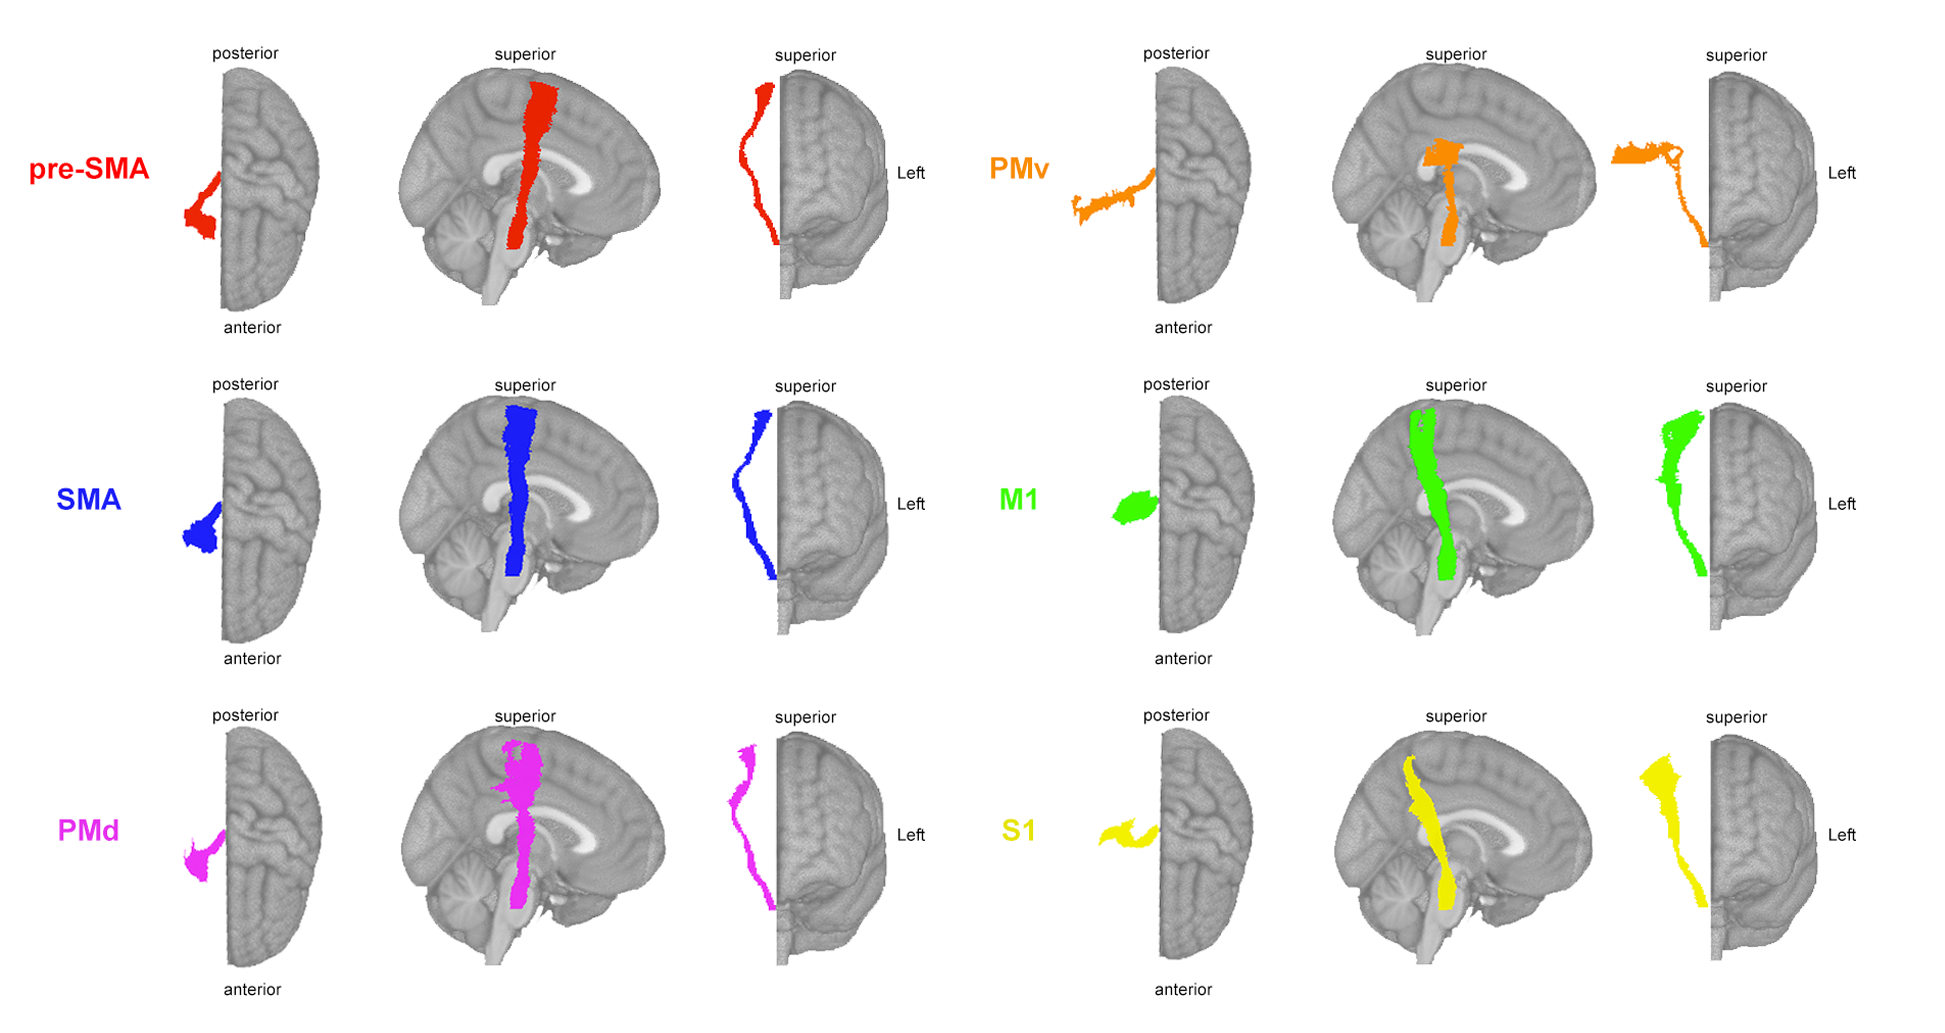
\includegraphics[width=1\linewidth]{figures/all_SMATT2.png}
    \caption{Sensorimotor tract template atlas (SMATT), displaying only right hemisphere tracts relative to an MNI template, including pre-supplementary motor area (pre-SMA), supplementary motor area (SMA), dorsal premotor cortex (PMd), ventral premotor cortex (PMv),  primary motor cortex (M1), and primary sensory cortex (S1). Pre-SMA is the most anterior tract, S1 is the most posterior tract.}
    \label{smatt}
  \label{fig:sfig1}
\end{subfigure}
\begin{subfigure}{1\textwidth}
  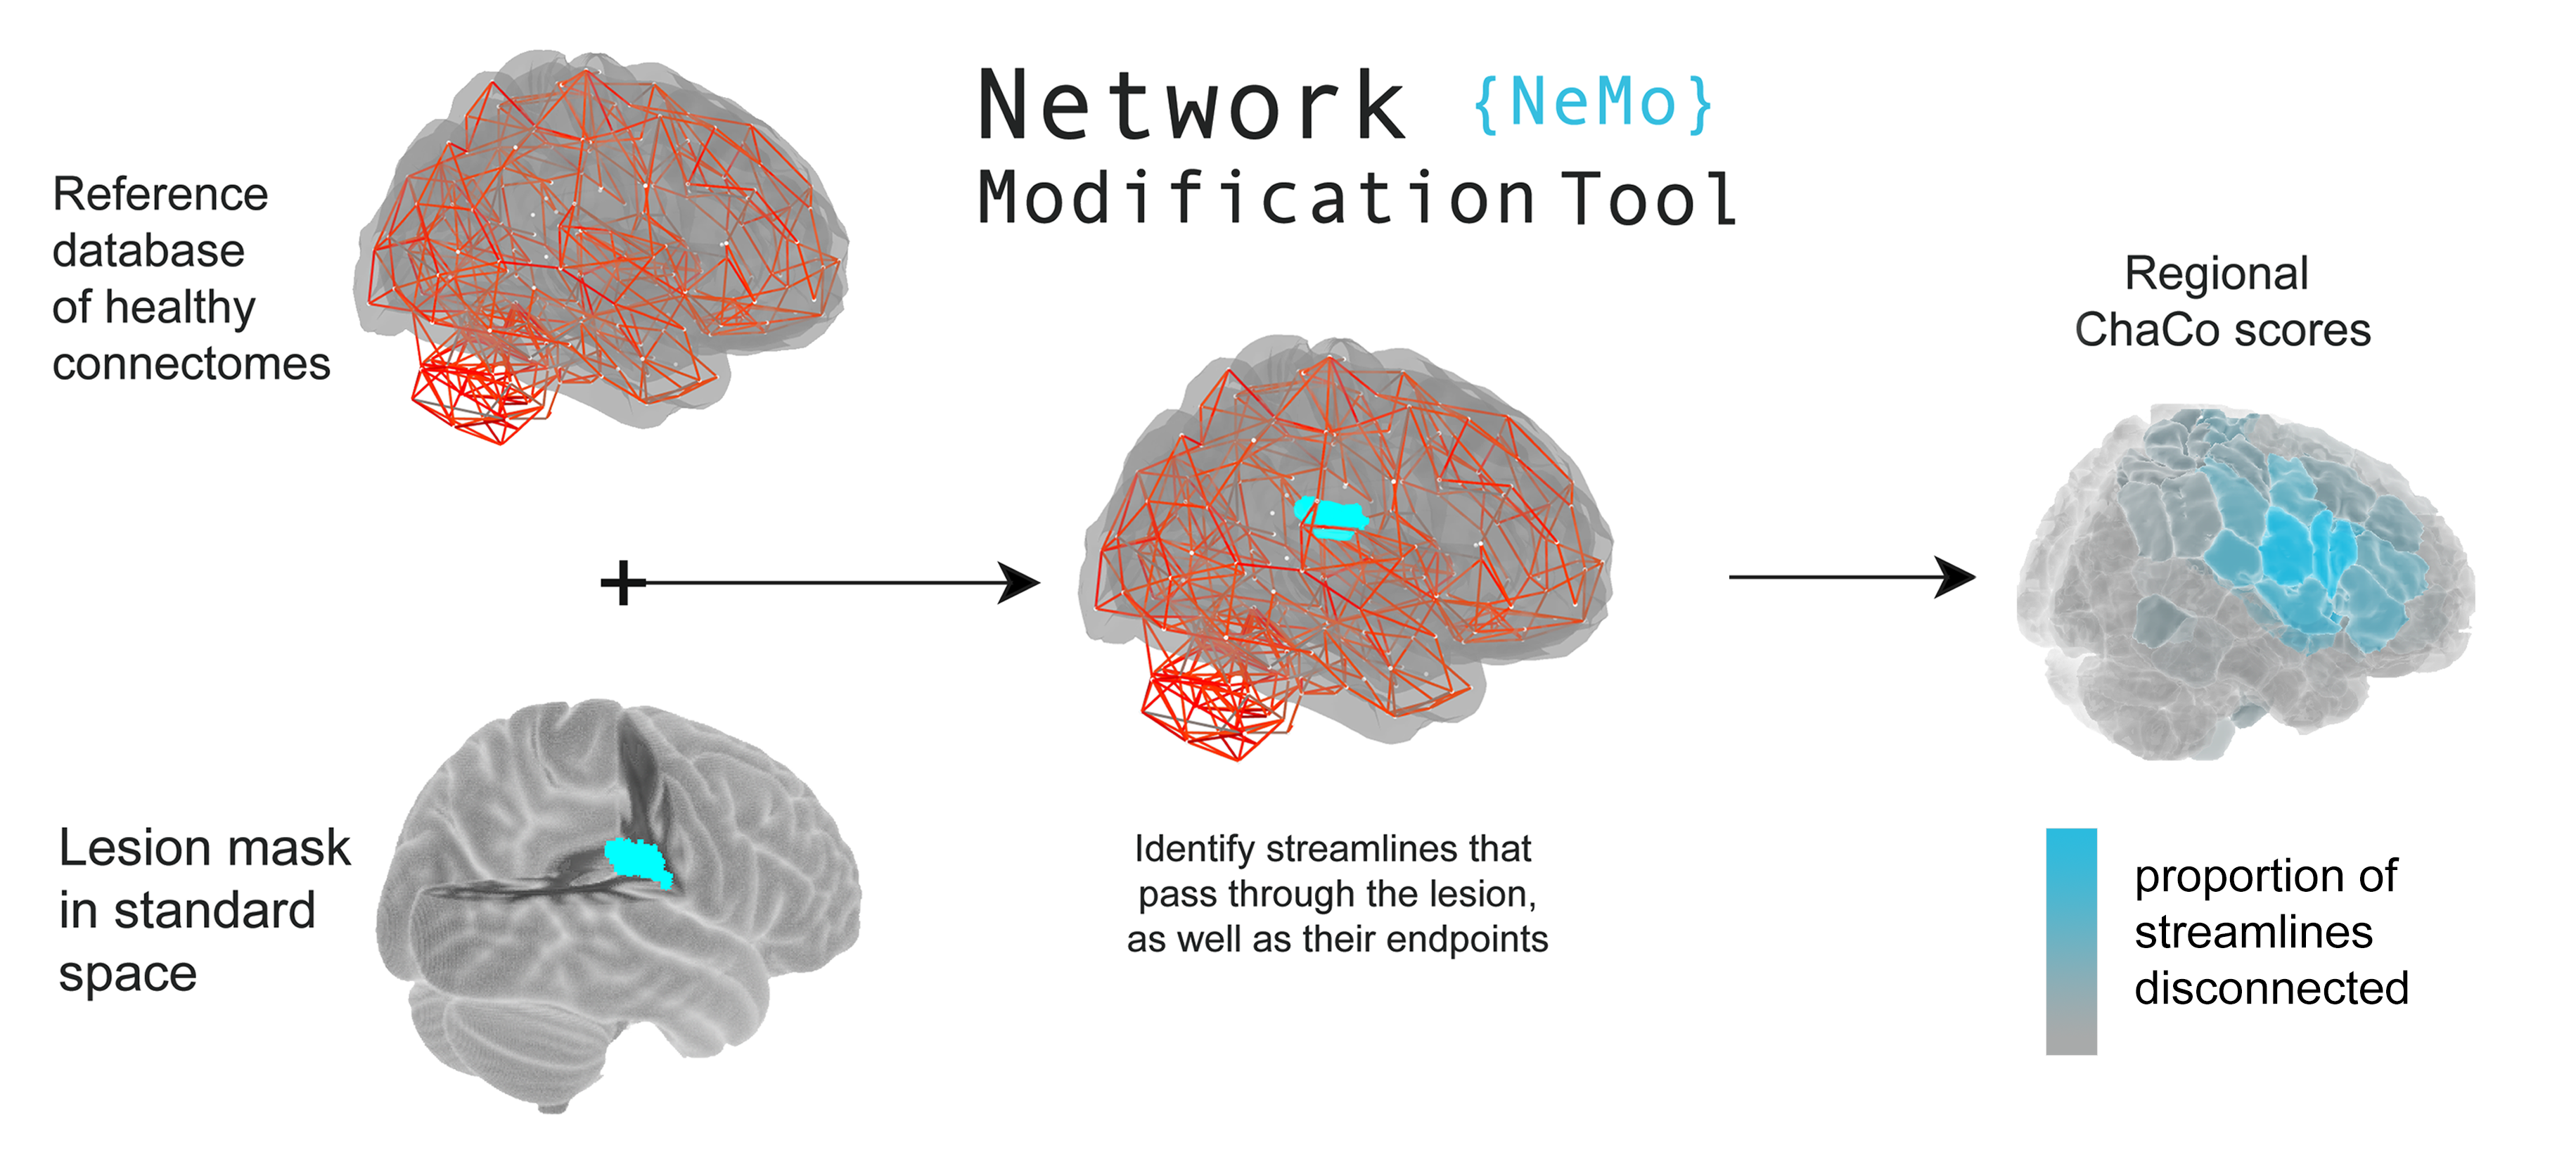
\includegraphics[width=1\linewidth]{figures/Multi-panelML_white_regional.png}
  \caption{Overview of the Network Modification (NeMo) tool. Binary lesion masks in MNI space representing the presence of a stroke lesion (turquoise) in a given voxel are provided by the user. Each lesion mask is embedded into 420 unrelated healthy structural connectomes (separately for each healthy subject) and the regional and pairwise change in connectivity (ChaCo) scores are calculated and averaged across healthy subjects (parcellation shown here is the Shen 268-region atlas). }
  \label{fig:sfig2}
\end{subfigure}
\caption{Overview of SMATT tracts and procedure for generating regional Change in Connectivity (ChaCo) scores using the Network Modification tool}
\label{smatt_and_chaco}
\end{figure}

Ridge regression models were used to predict chronic motor deficits from ipsilesional SMATT-LL (6 features) and from L/R-SMATT-LL (12 features). Ridge regression was used to account for multicollinearity of lesion load values between tracts (Supplementary Figure \ref{smatt_pairwise_correlations}, \ref{smatt_pairwise_correlations_bi}). Lesion load values were normalized (after train/test split) by subtracting the mean across subjects and dividing by the l2-norm prior to model fitting. In the inner loop, the degree of model regularization  ($\lambda$) was determined via grid-search over 30 values ranging from $10^-2$ to $10^2$. The training data was fit with the selected $\lambda$ and this model was used to predict motor scores for hold-out subjects in the test folds.

\subsubsection*{Structural lesion-network mapping (sLNM) models}
Structural lesion network maps were obtained from \cite{Bowren2022-rs}. Specifically, \cite{Bowren2022-rs} used sparse canonical correlation analysis to produce maps of white matter (WM) voxels in which damage was associated with Fugl-Meyer scores (\cite{Pustina2018-xv}). Then, tractography was seeded from these peak WM voxels to identify associated structural networks, called structural lesion network maps (sLNMs). Principal components analysis of sLNMs was performed, which produced 3 principal components that correspond to 5 sLNM maps (PC1, and positive/negative weights of PC2 and PC3). Lesion load on each sLNM map was calculated for each subject as the sum of the voxel intensities from the principal component map that intersected the lesion mask (Supplementary Figure \ref{slnm_distribution}). Ridge regression models were used to predict chronic motor deficits from sLNM lesion loads (5 features). As above, lesion load values were normalized (after train/test split) by subtracting the mean across subjects and dividing by the l2-norm prior to model fitting. In the inner loop, the degree of regularization on regression coefficients ($\lambda$) was determined via grid-search over 30 values ranging from $10^-2$ to $10^2$. The training data was fit with the selected $\lambda$ and this model was used to predict motor scores for hold-out subjects in the test folds. 

\subsubsection*{Regional change in connectivity (ChaCo) models}
Lesion masks in $1mm^3$ MNI v6 space were processed with the Network Modification Tool (NeMo Tool) v2 pipeline (\cite{Kuceyeski2013-nk}), available at https://kuceyeski-wcm-web.s3.us-east-1.amazonaws.com/upload.html; see https://github.com/kjamison/nemo for documentation. Given a lesion mask, the NeMo tool produces outputs that reflect the impact of the lesion on white matter tracts using healthy structural connectomes as a reference. The NeMo tool embeds a lesion mask into healthy structural connectomes, identifies all white matter streamlines that intersect with the lesion, and determines the brain regions at the endpoints of those streamlines (Figure \ref{smatt_and_chaco}B). Regional change in connectivity (ChaCo) scores, or the ratio of the number of disrupted streamlines divided by the total number of streamlines terminating in each region, were calculated for all gray matter regions (see Supplementary Figure \ref{mean_std_chaco}A,B for distribution of mean and standard deviation of ChaCo scores). The NeMo tool uses structural connectivity from 420 unrelated subjects from the Human Connectome Project Young Adult database. For each stroke lesion, the NeMo tool calculates regional ChaCo scores for all HCP subjects separately and then produces final regional ChaCo scores by taking the mean across HCP subjects. Structural connectivity in HCP subjects was obtained using deterministic tractography (SD stream) with dynamic seeding, with additional SIFT2 weighting for each of 5 million streamlines (\cite{Smith2015-eb}). Regional ChaCo scores from two different altases were compared: the 86-region Desikan-Killiany Atlas (68 cortical regions $\Plus$ 18 subcortical regions, excluding brainstem) from FreeSurfer ("fs86" for short), which contains coarse anatomically parcellated regions (\cite{Desikan2006-vf,Fischl2002-lb}), and the 268-region Shen atlas ("shen268" for short), which contains more fine-grained functionally parcellated cortical and subcortical regions (\cite{Shen2013-zn}).

First, the performance of ridge regression models was assessed, as described above, with regional ChaCo scores as inputs (86 features for the fs86 atlas, 268 features for the shen268 atlas). Second, a filter-based feature selection step was added to the ridge regression models to obtain a subset of features that were the most useful for prediction (\cite{Guyon2003-kj, Hall1999-qr, Pudjihartono2022-zg}). Features were ranked by their their association with the outcome variable (p-value from univariate correlation) and only the $\kappa$ most associated variables were included in the model. In the inner hyperparameter selection loop, both the amount of regularization on regression coefficients ($\lambda$) and the number of features to retain in the model ($\kappa$) were selected via grid search. The $\lambda$ value was chosen by searching over 30 values ranging $10^-2$ to $10^2$, and the $\kappa$ value was chosen by searching 30 values ranging from 5 to the maximum number of features possible (for fs86: 86, for shen268: 268) in base-2 steps.  This feature selection approach was implemented to identify sparse sets of correlated variables, as opposed to more basic embedded feature selection techniques such as LASSO (\cite{Tibshirani1996-sk}) that randomly suppresses collinear features. Retaining only one of several correlated features may impact performance of the model in predicting scores for novel subjects with different lesion topographies. Furthermore, retaining redundant features (i.e., features that have high collinearity with other features) may specifically benefit predictive lesion-deficit mapping, as we expect to observe meaningful clusters of correlated damage in brain regions that share the same general vascular territory.

\subsubsection*{Ensemble models}

We tested whether models including demographic information (age, sex, and days post stroke), ensembled with lesion models, perform better than models with lesion data or demographic data alone (i.e., we hypothesized that the variance explained from lesion data and demographic data is not redundant). We also assessed whether models including both lesion load and ChaCo scores will perform better than models with lesion load or ChaCo scores alone. The idea of ensemble learning is to build a single prediction model by combining the strengths of a collection of simpler base models; we used ensemble models that average predictions from different biomarkers (\cite{Hastie2001-or}).

Ensemble models were generated by training ChaCo-models and lesion load models separately, on the same subjects and with the same training/test/validation splits, and averaging the final predicted scores for each test subject. A standard linear regression model was used to model the relationship between demographic information and motor impairment. 

\subsubsection*{Model comparisons}
Differences in performance between models were assessed using two-sided Mann-Whitney U tests and p-values were corrected for multiple comparisons using Bonferroni correction. 

\subsubsection*{Consistency of feature weights}
The stability of the model coefficients $\beta$ for the best-performing models was assessed as follows. For the 86-region ChaCo models, the average of the 86-region $\beta$ vector across 5 folds was calculated for each permutation. This represents the average $\beta$ of the 5 best-performing models across cross-validation splits. The distribution of the average $\beta$ coefficients of all features across 100 permutation was visualized. For the 268-region ChaCo models with feature selection, the most consistently-selected features (selected in at least 475/500 folds or 99$\%$ of folds, heuristically) were identified and the average of the $\beta$ vector across the 5 folds was calculated for each permutation. The distribution of the average $\beta$ coefficients of consistently-selected features across 100 permutations was visualized. 

\subsubsection*{Code details}
The scikit-learn package was used to implement machine learning models (http://scikit-learn.org). All analysis scripts that generated the results of the present study are readily accessible and open for reuse (https://github.com/emilyolafson/lesion$\_$predictions). The script can be easily modified to predict any outcome score from ChaCo scores/lesion load data.

\section{Results}


\begin{figure}[htp]
\centering
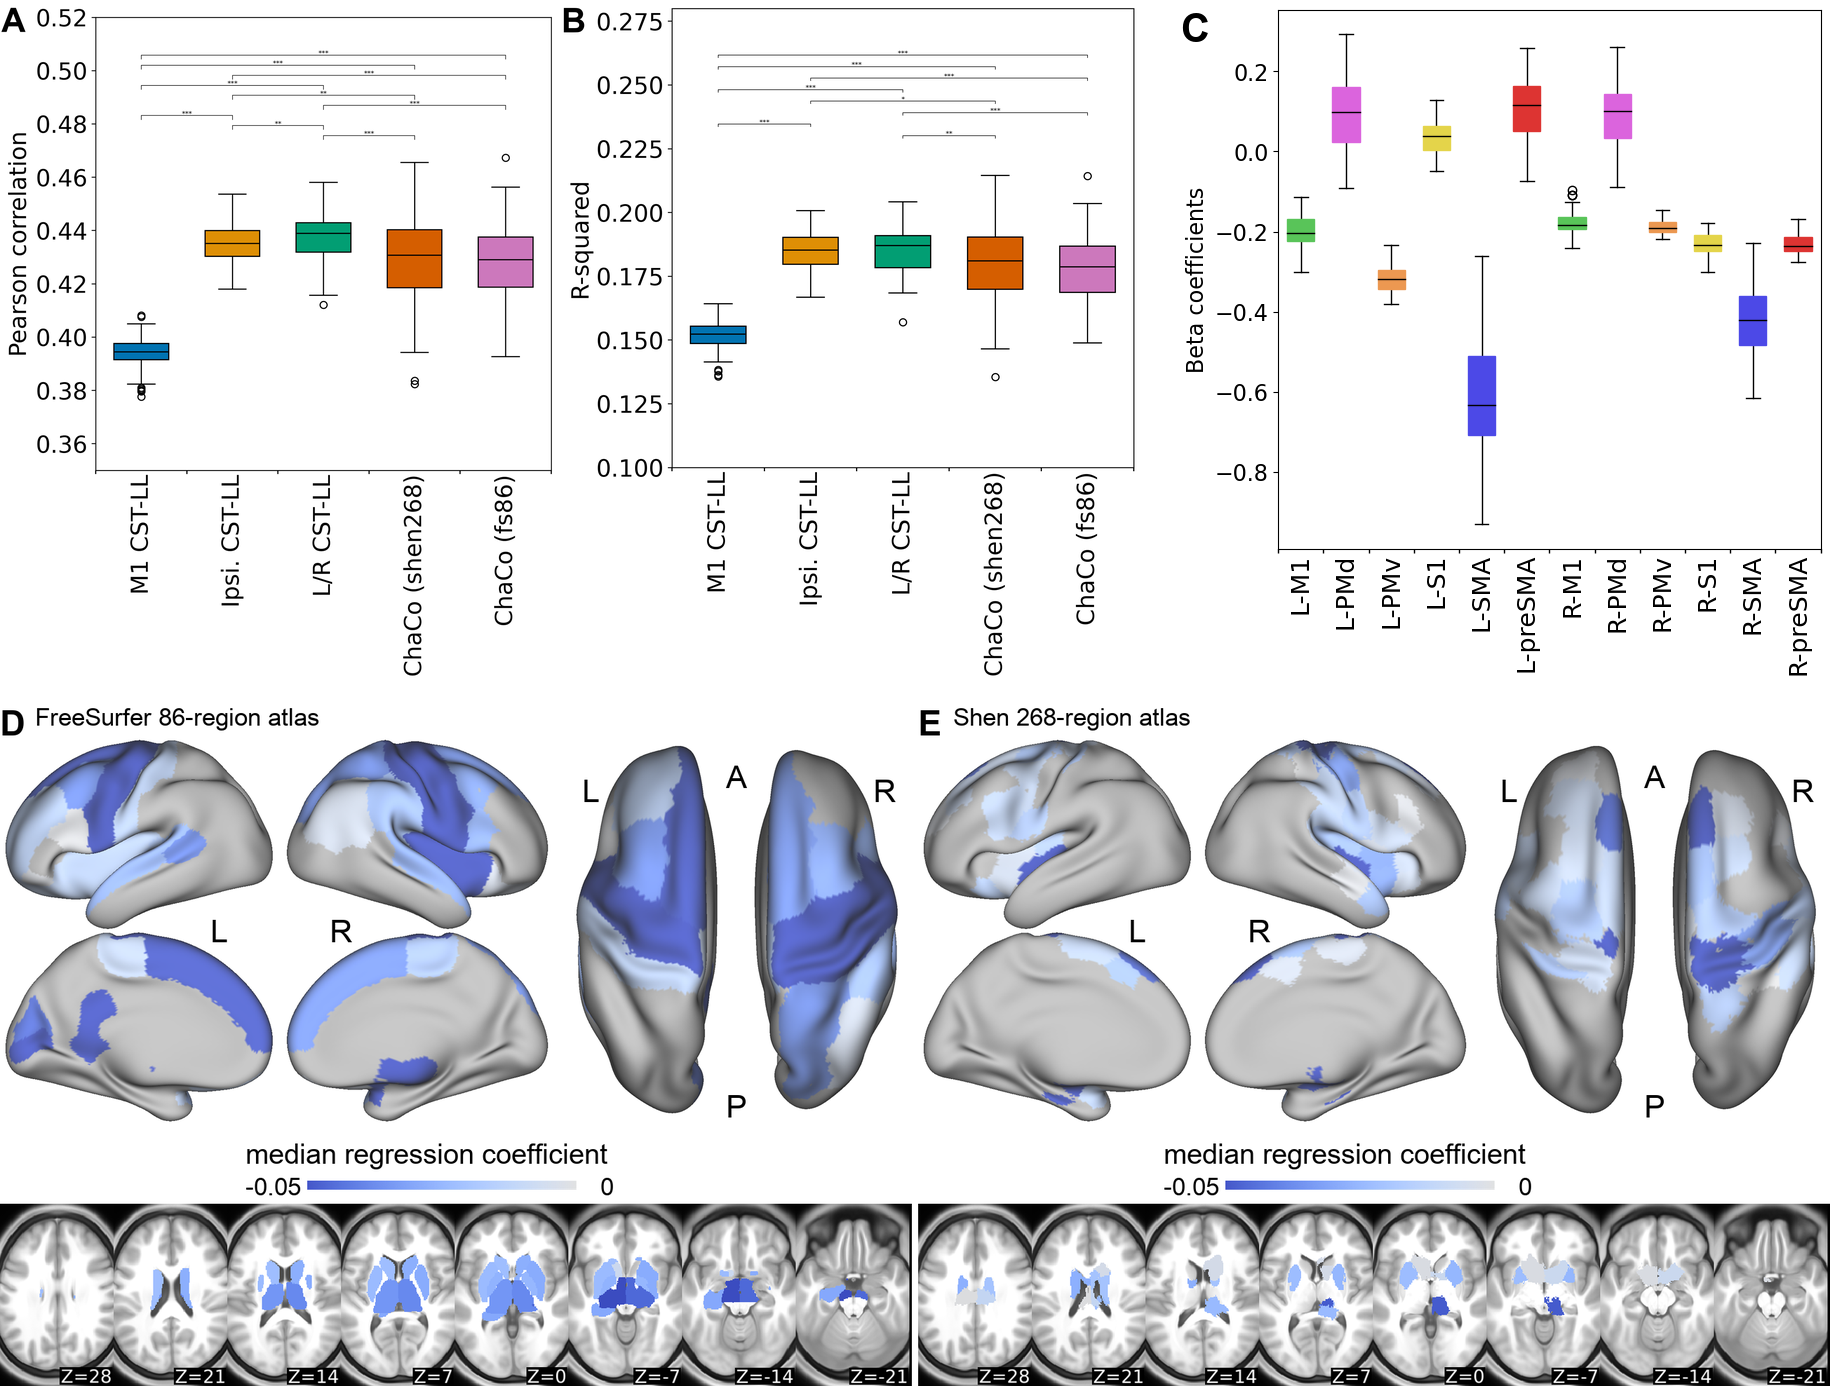
\includegraphics[width=1\linewidth]{figures/Analysis1.png}
\caption{Summary of model performance metrics across all models tested and feature weights (regression coefficients $\beta$) for the two best-performing models.  \textbf{A.} and \textbf{B.} Distribution of model performance (mean Pearson correlation/$R^2$ across 5 outer folds for 100 permutations of the data).  Boxplots are colored arbitrarily for clarity and are plotted in similarly-colored pairs to indicate performance using the full training data ("Acute $\Plus$  chronic") versus only chronic data ("Chronic only"). The boxes extend from the lower to upper quartile values of the data, with a line at the median. Whiskers represent the range of the data from [Q1-1.5*IQR, Q3+1.5*IQR].
\textbf{C.} and \textbf{D.} Mean feature weights for the top two best-performing models (ChaCo (fs86) without feature selection, ChaCo (shen268) with feature selection, respectively). For the fs86-ChaCo model (left), we display the mean regression coefficients  $\beta$ across 100 permutations. For ChaCo (shen268) (right), we display the median regression coefficients of regions that were selected in at least 95$\%$ of outer folds (i.e., for regions that were included in the model in at least 475/500 outer folds, mean $\beta$ coefficients were calculated across 5 outer folds, and the median value across 100 permutations is plotted). }
\label{analysis1}
\end{figure}

The out-of-sample performances of the models can be found in Figure \ref{analysis1}A,B. In general, M1 CST-LL, SMATT-LL, and sLNM-LL performed worse on average than ChaCo models, with Left/Right SMATT-LL models performing the best among them (correlation = 0.446, $R^2$ = 0.188) and M1 CST-LL models performing the worst (correlation = 0.395, $R^2$ = 0.133, n.s. between chronic and mixed training data). 

Regional ChaCo scores from the 268-region Shen atlas best predicted chronic motor scores in unseen subjects. In particular, the best performance with this model was obtained using acute and chronic data for training plus feature selection (correlation = 0.467, $R^2$ = 0.210). $\beta$ coefficients for selected features were consistent in direction and magnitude across permutations (Supplementary Figure \ref{shen_beta_coeffs})). The performance of this model was on par with a model using regional ChaCo scores from the 86-region FreeSurfer atlas, that also used acute and chronic data for training and no feature selection (correlation = 0.458, $R^2$ = 0.204, n.s. between models). $\beta$ coefficients for all regions were consistent in direction and magnitude across permutations (Supplementary Figure  \ref{shen_beta_coeffs})).  Thus, the effect of feature selection in ChaCo models depended on the atlas: for the lower-dimension 86-region FreeSurfer atlas, feature selection reduced model performance, whereas for the higher dimension 268-region Shen atlas, feature selection improved it. 

\begin{figure}[hp]
\centering
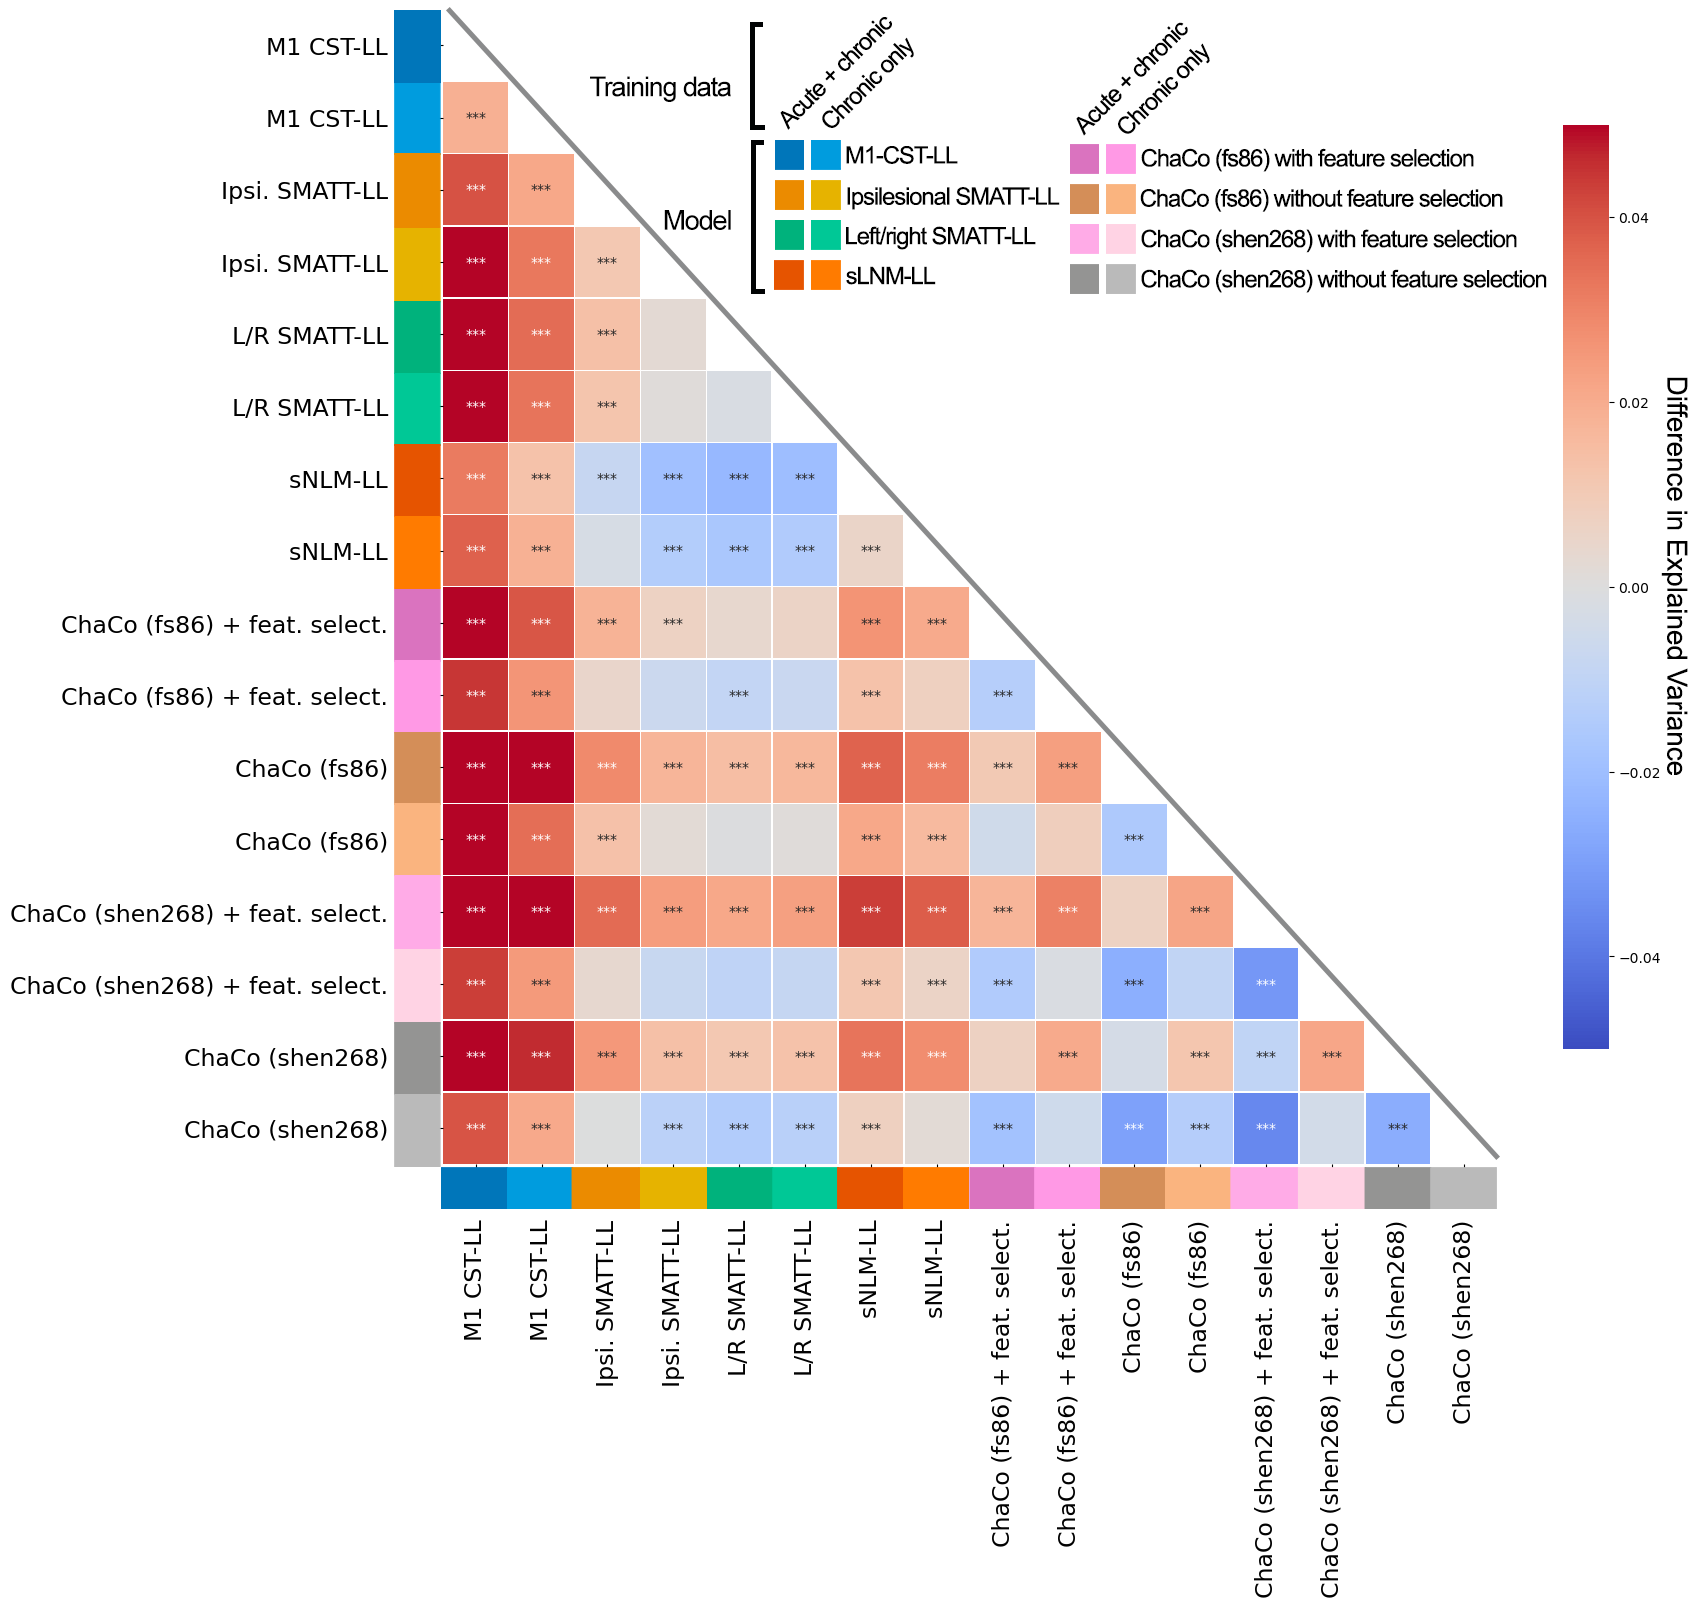
\includegraphics[width=1\linewidth]{figures/analysis_1_matrix_figure_colors.png}
\caption{Statistical comparison of model performance for predicting motor scores via averaging the difference in explained variance for each of the 100 cross-validation splits to ensure models being compared used the same train/test data. Significance was determined using exact tests for differences. $***$ denotes corrected $p < 0.001$, $**$ denotes corrected $p < 0.01$, $*$ denotes corrected $p < 0.05$ after Bonferroni correction. A positive difference indicates that the model on the y-axis (vertical) has a greater explained variance than the model on the x-axis (horizontal).
 }
\label{analysis1}
\end{figure}

Model weights for the best-performing ChaCo models are shown in (Figure \ref{analysis1}C, D), reflecting median $\beta$ coefficients for regions selected in least 475/500 outer folds of the 268-region ChaCo models. There were several spatial similarities in the pattern of feature weights for the 86-region ChaCo model and 268-region ChaCo model with feature selection. For both atlases, negative model weights (indicating more disconnection = worse motor outcomes) are assigned to superior portions of left and right motor areas, as well as in subcortical structures like the putamen, pallidum, and thalamus, whereas positive weights are assigned to frontal and parietal areas. In the 268-region ChaCo models, more regions in the right hemisphere are consistently included in the model than the left hemisphere. 


For ChaCo models using the shen 268-region atlas with feature selection, on average 110 features were selected (Supplementary Figure \ref{lambda_kappa}). A hierarchically-clustered heatmap of the correlation matrix of the selected features (Supplementary Figure \ref{heatmap_shen_negweights}) shows that many of the selected features are clustered (i.e., high correlation in ChaCo scores across subjects), and are frequently damaged together. Additionally, ChaCo scores of regions with positive and negative regression weights were positively correlated across subjects, despite these features having opposite relationships to motor deficits (Supplementary Figure \ref{heatmap_shen_pos_vs_negative}). For ChaCo models using the FreeSurfer 86-region atlas with feature selection, in the majority of cross-validation folds, all 86 regions were selected in the model. 

Including additional acute subjects in the training data improved model performance for left/right SMATT-LL model and for ChaCo models. However, performance remained the same or was reduced for M1-CST-LL models, ipsilesional SMATT-LL models and sLNM models.

Generally, ensemble models performed marginally better than individual models (Figure \ref{analysis2_boxplots} and Table \ref{results_table_acutechronic}). In particular, including demographic information increased or did not change prediction accuracy for all models tested, and combining ChaCo models with lesion load models improved performance.  The best performance was obtained by combining L/R SMATT lesion load with 268-region ChaCo models with feature selection (L/R SMATT-LL + ChaCo (shen268) w/ feat. select $R^2 = 0.233$, L/R SMATT-LL $R^2=0.188$, ChaCo (shen268) w/ feat. select, $R^2=0.210$).\\

\begin{table}[h]
\centering
\label{table:5}
\begin{tabular}{lrrrr}
\toprule
 &  & \multicolumn{2}{c}{Median performance} \\
Ensemble type & Model name & Correlation & $R^2$  \\
\midrule
\multirow[t]{8}{*}{None} &  M1 CST-LL & \colorBlack{0.395} & \colorBlack{0.133} \\
 & Ipsi. SMATT-LL & \colorBlue{0.430} & \colorBlack{0.174} \\
 & L/R SMATT-LL & \colorBlue{0.446} & \colorBlack{0.188} \\
 & sLNM-LL & \colorBlue{0.428} & \colorBlack{0.167} \\
 & ChaCo (fs86) & \colorBlue{0.458} & \colorBlue{0.204} \\
 & ChaCo (shen268) & \colorBlue{0.456} & \colorBlack{0.199} \\
 & ChaCo (fs86) (feat. select.) & \colorBlue{0.447} & \colorBlack{0.191} \\
 & ChaCo (shen268) (feat. select.) & \colorNavyBlue{0.468} & \colorBlue{0.210} \\
 \hline
\multirow[t]{8}{*}{$\Plus$ Demographics} & M1 CST-LL + demog. & \colorBlue{0.424} & \colorBlack{0.173} \\
 & Ipsi. SMATT-LL + demog. & \colorBlue{0.457} & \colorBlack{0.199} \\
 & L/R SMATT-LL + demog. & \colorNavyBlue{0.462} & \colorBlue{0.203} \\
 & sLNM-LL + demog. & \colorBlue{0.452} & \colorBlack{0.191} \\
 & ChaCo (fs86) + demog & \colorNavyBlue{0.471} & \colorBlue{0.203} \\
 & ChaCo (shen268) + demog & \colorNavyBlue{0.468} & \colorBlue{0.204} \\
 & ChaCo (fs86) (feat. select.) + demog & \colorNavyBlue{0.465} & \colorBlue{0.201} \\
 & ChaCo (shen268) (feat. select.) + demog & \colorNavyBlue{0.481} & \colorBlue{0.215} \\
 \hline
\multirow[t]{16}{*}{Lesion load $\Plus$} & M1 CST-LL + ChaCo (fs86subj) & \colorNavyBlue{0.461} & \colorBlue{0.210} \\
 ChaCo & M1 CST-LL + ChaCo (shen268) & \colorNavyBlue{0.463} & \colorBlue{0.211} \\
 & Ipsi. SMATT-LL + ChaCo (fs86subj) & \colorNavyBlue{0.478} & \colorNavyBlue{0.226} \\
 & Ipsi. SMATT-LL + ChaCo (shen268) & \colorNavyBlue{0.481} & \colorNavyBlue{0.228} \\
 & L/R SMATT-LL + ChaCo (fs86subj) & \colorNavyBlue{0.481} & \colorNavyBlue{0.227} \\
 & L/R SMATT-LL + ChaCo (shen268) & \colorNavyBlue{0.481} & \colorNavyBlue{0.228} \\
 & sLNM-LL + ChaCo (fs86subj) & \colorNavyBlue{0.468} & \colorBlue{0.214} \\
 & sLNM-LL + ChaCo (shen268) & \colorNavyBlue{0.472} & \colorBlue{0.217} \\
 & M1 CST-LL + ChaCo (fs86subj) (feat. select.) & \colorBlue{0.458} & \colorBlue{0.206} \\
 & M1 CST-LL + ChaCo (shen268) (feat. select.) & \colorNavyBlue{0.469} & \colorBlue{0.217} \\
 & Ipsi. SMATT-LL + ChaCo (fs86subj) (feat. select.) & \colorNavyBlue{0.476} & \colorNavyBlue{0.223} \\
 & Ipsi. SMATT-LL + ChaCo (shen268) (feat. select.) & \colorNavyBlue{0.485} & \colorProcessBlue{0.233} \\
 & L/R SMATT-LL + ChaCo (fs86subj) (feat. select.) & \colorNavyBlue{0.475} & \colorNavyBlue{0.222} \\
 & L/R SMATT-LL + ChaCo (shen268) (feat. select.) & \colorNavyBlue{0.486} & \colorProcessBlue{0.232} \\
 & sLNM-LL + ChaCo (fs86subj) (feat. select.) & \colorNavyBlue{0.462} & \colorBlue{0.208} \\
 & sLNM-LL + ChaCo (shen268) (feat. select.) & \colorNavyBlue{0.474} & \colorNavyBlue{0.222} \\
 \hline
\multirow[t]{16}{*}{Lesion load $\Plus$} & M1 CST-LL + ChaCo (fs86subj) + demog. & \colorNavyBlue{0.476} & \colorBlue{0.214} \\
 ChaCo $\Plus$ & M1 CST-LL + ChaCo (shen268) + demog. & \colorNavyBlue{0.477} & \colorBlue{0.216} \\
 Demographics & Ipsi. SMATT-LL + ChaCo (fs86subj) + demog. & \colorProcessBlue{0.492} & \colorProcessBlue{0.230} \\
 & Ipsi. SMATT-LL + ChaCo (shen268) + demog. & \colorProcessBlue{0.495} & \colorProcessBlue{0.232} \\
 & L/R SMATT-LL + ChaCo (fs86subj) + demog. & \colorProcessBlue{0.494} & \colorProcessBlue{0.231} \\
 & L/R SMATT-LL + ChaCo (shen268) + demog. & \colorProcessBlue{0.494} & \colorProcessBlue{0.232} \\
 & sLNM-LL + ChaCo (fs86subj) + demog. & \colorNavyBlue{0.484} & \colorNavyBlue{0.222} \\
 & sLNM-LL + ChaCo (shen268) + demog. & \colorNavyBlue{0.487} & \colorNavyBlue{0.224} \\
 & M1 CST-LL + ChaCo (fs86subj) (feat. select.) + demog. & \colorNavyBlue{0.472} & \colorBlue{0.212} \\
 & M1 CST-LL + ChaCo (shen268) (feat. select.) + demog. & \colorNavyBlue{0.482} & \colorNavyBlue{0.222} \\
 & Ipsi. SMATT-LL + ChaCo (fs86subj) (feat. select.) + demog. & \colorProcessBlue{0.490} & \colorNavyBlue{0.228} \\
 & Ipsi. SMATT-LL + ChaCo (shen268) (feat. select.) + demog. & \colorProcessBlue{0.498} & \colorProcessBlue{0.237} \\
 & L/R SMATT-LL + ChaCo (fs86subj) (feat. select.) + demog. & \colorProcessBlue{0.490} & \colorNavyBlue{0.229} \\
 & L/R SMATT-LL + ChaCo (shen268) (feat. select.) + demog. & \colorProcessBlue{0.499} & \colorProcessBlue{0.237} \\
 & sLNM-LL + ChaCo (fs86subj) (feat. select.) + demog. & \colorNavyBlue{0.479} & \colorBlue{0.218} \\
 & sLNM-LL + ChaCo (shen268) (feat. select.) + demog. & \colorProcessBlue{0.492} & \colorProcessBlue{0.230} \\
\bottomrule
\end{tabular}
\caption{Test performance of all models evaluated, displaying median $R^2$ and median correlation of average hold-out performances (i.e. average across 5 outer folds) across 100 permutations. Demog. = demographics, Ipsi. = Ipsilesional, SMATT LL = sensorimotor tract template lesion load, L/R SMATT LL = left and right sensorimotor tract template lesion load, M1 CST LL = M1 corticospinal tract lesion load, ChaCo = Change in Connectivity, fs86 = FreeSurfer 86-region atlas, feat. select. = feature selection}
\label{results_table_acutechronic}
\end{table}




\begin{figure}[htp]
\centering
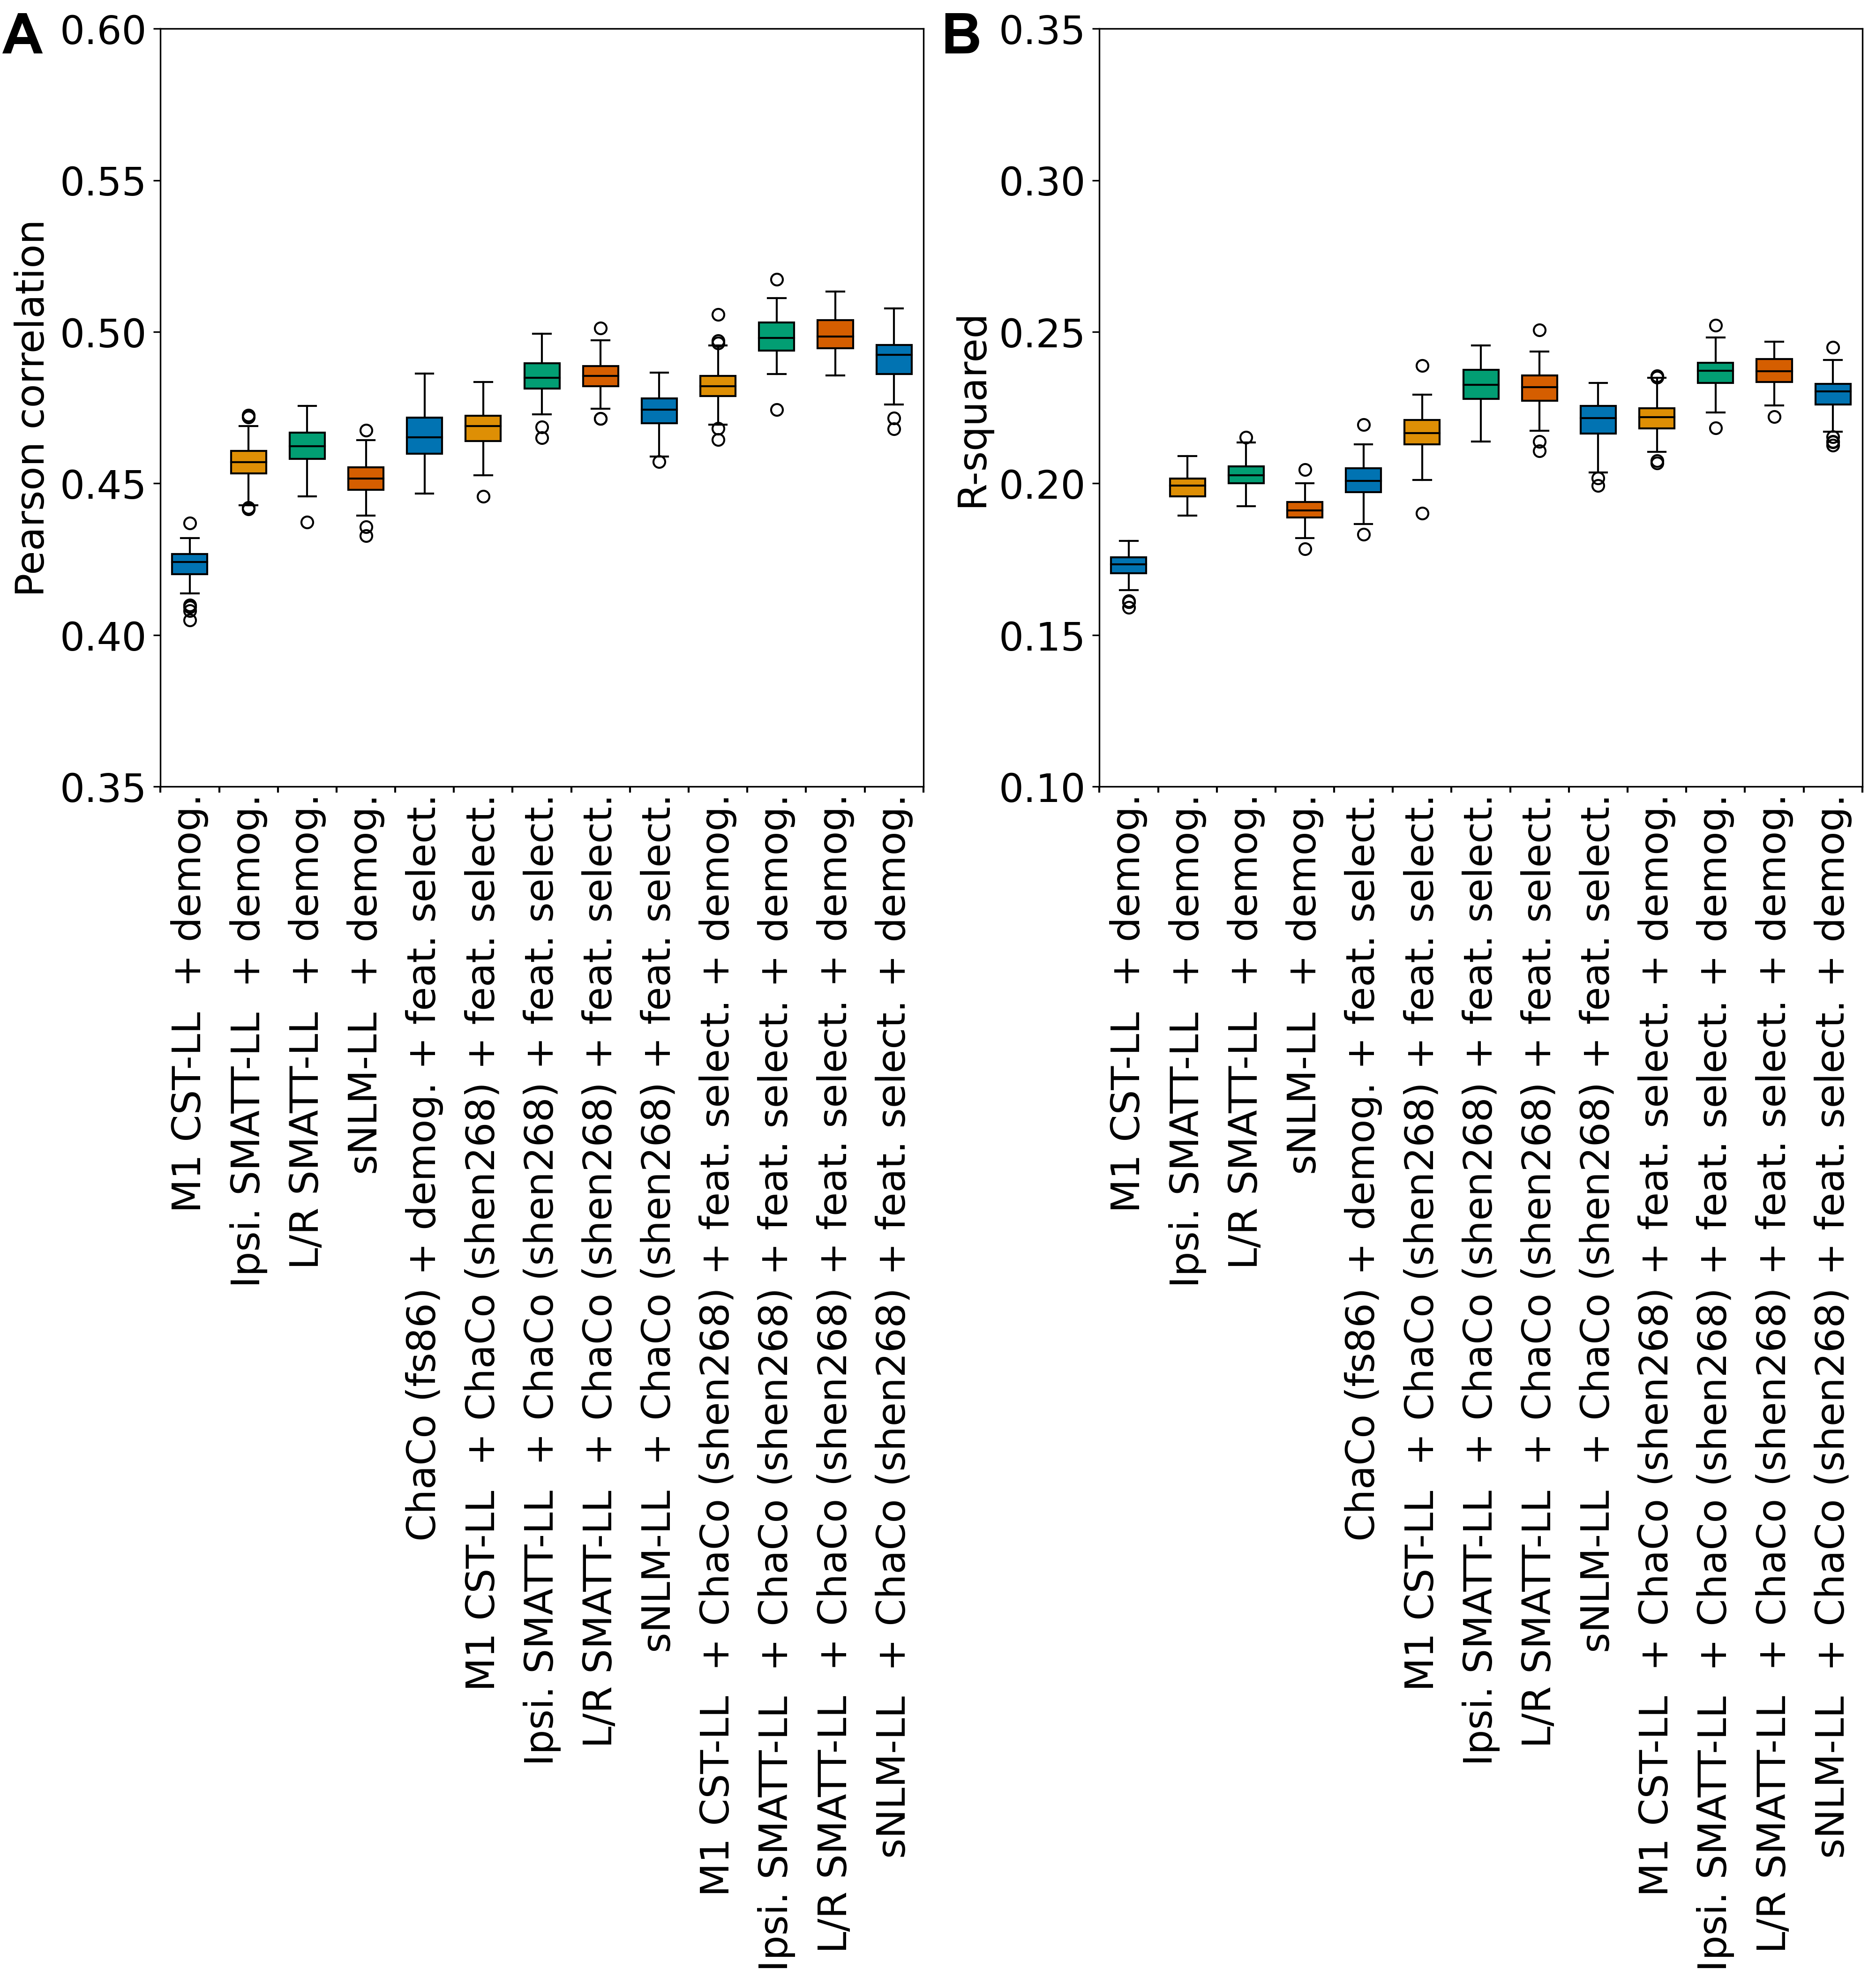
\includegraphics[width=1\linewidth]{figures/Analysis2_boxplots.png}
\caption{Distribution of ensemble model performance, using acute and chronic data for training. \textbf{A} and \textbf{B} show the distribution of model performances (mean Pearson correlation/$R^2$ across 5 outer folds for 100 permutations of the data). Boxplots are colored arbitrarily for clarity. The boxes extend from the lower to upper quartile values of the data, with a line at the median. Whiskers represent the range of the data from [Q1-1.5*IQR, Q3+1.5*IQR].  Demog. = demographics, Ipsi. = Ipsilesional, SMATT LL = sensorimotor tract template lesion load, L/R SMATT LL = left and right sensorimotor tract template lesion load, M1 CST LL = M1 corticospinal tract lesion load, ChaCo = Change in Connectivity, fs86 = FreeSurfer 86-region atlas, feat. select. = feature selection}
\label{analysis2_boxplots}
\end{figure}

\begin{figure}[htp]
\centering
\includegraphics[width=1\linewidth]{figures/Analysis2_matrix.png}
\caption{Statistical comparison of model performance for ensemble models. Difference in explained variance between pairs of models using different lesion metrics and different training data. Model differences were calculated by averaging the difference in explained variance for each of the 100 train/test splits so models built and tested on the same data are compared. Significance of differences in explained variance were evaluated using exact tests; $***$ denotes corrected $p < 0.001$, $**$ denotes corrected $p < 0.01$, $*$ denotes corrected $p < 0.05$ after Bonferroni correction. A positive difference value indicates that the model on the y-axis (vertical) has a greater explained variance than the model on the x-axis (horizontal).}
\label{analysis2_matrix}
\end{figure}

\section{Discussion}
In this study, we compared the performance of models predicting post-stroke motor ability built using several structural imaging biomarkers derived from a large, multi-site dataset. We found that modelling lesion damage using regional ChaCo scores, using correlation-based feature selection and data from both acute and chronic subjects resulted in a model that best predicted chronic motor scores. Models using features derived from multivariate voxelwise lesion-behaviour modelling performed worse than more basic models using lesion load on the descending corticospinal tract. Finally, we saw that combining several biomarkers and demographic information using ensemble modelling improved prediction of post-stroke motor ability.

\subsubsection*{Higher-order motor areas are relevant for motor outcome prediction}
This study supports previous results showing that M1-CST-LL alone does not capture enough variance to accurately predict chronic post-stroke motor outcomes(\cite{Rondina2017-ij, Park2016-te, Ito2022-em}), although few studies have directly compared the out-of-sample performance of M1-CST-LL against more complex metrics like those assessed in this paper. Corticospinal projections consist of fibers originating not just from M1, but from higher order motor areas in the frontal and parietal lobes (\cite{Galea1994-yi}) that have been implicated in motor planning and execution (\cite{Ball1999-yo}). Damage to descending fibers from these areas has been associated with motor deficits after stroke (\cite{Ito2022-em, Riley2011-xo}) and may explain additional variance in chronic motor outcome that is not captured by damage to the M1 corticospinal tract alone. Furthermore, preserving hemispheric information (i.e. in L/R SMATT-LL models) improved prediction performance above ipsilesional SMATT-LL, suggesting that there may be differential associations between motor tract damage and motor outcomes in each hemisphere.  This finding is also supported by the asymmetric feature weights in the left and right hemisphere in the ChaCo models. M1-CST-LL is currently the only structural neuroimaging biomarker recommended for clinical trials (\cite{Boyd2017-gs}); this study supports the notion that further development of non-M1-CST biomarkers is justified and that taking into account damage to non-primary motor regions is important for understanding variation in motor outcome.

\subsubsection*{Lesion-based structural disconnectivity for prediction}

Models using ChaCo scores performed best of all models tested, particularly when feature selection was employed. ChaCo scores can can capture both white matter and gray matter damage (\cite{Kuceyeski2013-nk}), which may enable them to capture relevant information for predicting motor deficits (\cite{Park2016-te,Rondina2016-ds}) that are not captured with lesion load metrics of white matter tract damage. 

Another strength of models using ChaCo scores can be understood, in part, by considering their superior performance compared to sLNM models. In both models, features reflecting lesion-induced damage were selected on the basis of those that contributed to the prediction of motor deficits in a held-out sample; i.e., the features were selected in a data-driven way. Similarly, in both models, lesion-induced white matter damage is the primary feature of interest. One difference lies in how lesion-induced white matter damage is calculated. The sLNM maps represent white matter tracts that pass through voxels important for predictions, and the data on which feature selection takes place are voxels. On the other hand, in ChaCo models, the data on which feature selection takes place are regional measures of structural disconnection. Statistical power may be increased when voxelwise lesion data is first transformed into regional ChaCo scores; non-overlapping lesions that affect different portions of the same tract are mapped onto ChaCo scores of the same region or set of regions. This data transformation essentially reduces the number of "rare" features compared to voxelwise representations, and can be qualitatively seen in the distribution of the standard deviation of ChaCo scores across subjects (Supplementary Figure \ref{mean_std_chaco}) and the histogram of ChaCo damage compared to the distribution of lesion damage (Supplementary Figure \ref{histogram_voxels_chaco}). The drawback to this approach is that regional ChaCo scores do not enable the detection of associations between damage to specific tracts and motor outcomes; if such associations exist then that signal may be diluted in regional measures. 

Although this is one of few studies to use regional structural disconnectivity measures to predict stroke outcomes (see also \cite{Tozlu2020-qa, Kuceyeski2016-vj}), it finds its conceptual home among other voxelwise structural disconnection-behavior mapping approaches for inference and prediction (\cite{Salvalaggio2020-pe, Wawrzyniak2022-kl, Foulon2018-bj, Sperber2022-oj}). Structural disconnection-behaviour mapping has been recently employed to identify white matter correlates of behaviour (\cite{Wawrzyniak2022-kl, Foulon2018-bj}), and to predict 2-week motor scores from lesion-induced pairwise structural disconnection (\cite{Salvalaggio2020-pe}). In the latter, most conceptually similar to this study, tractography is seeded from voxels in a lesion, and a map representing the probability of disconnection from the lesion is generated. Features for ridge regression models are generated via principal components analysis (PCA) on the voxelwise structural disconnectivity maps. This is a reasonable dimensionality reduction step that has been applied in voxelwise lesion-symptom mapping to identify primary axes of variance of disconnectivity (\cite{Ivanova2021-nh}), but is a fundamentally different approach for representing structural disconnection compared to the NeMo tool, which reduces dimensionality by summarizing the degree of disconnection for each brain region separately. As demonstrated in this paper, regions that are frequently damaged together (and whose tracts may be loaded onto the same principal component in the PCA approach) may have opposite relationships to motor scores, so dimensionality reduction steps based on shared variance that do not consider relationships between structural disconnections and outcome variables may compress relevant individual signals into single features, reducing the predictive performance of a model. 

\subsubsection*{Features important in the ChaCo models}

In this paper, we are explicitly not attempting to do inference on the set of features that were selected by the model; however, further investigation into the features chosen along with their weights can provide some clarity in understanding the model's performance. Correlation-based feature selection is known to choose redundant features (\cite{Guyon2003-kj})). Indeed, damage to many selected regions is highly correlated, suggesting that information from these regions is somewhat redundant. Does this mean that our model is suboptimal, and that fewer features are actually necessary for good predictions? No; in the context of lesion-deficit modelling, damage to adjacent regions can be highly correlated because they are supplied by the same vascular territory, and a stroke in that artery will cause damage to both areas (\cite{Mah2014-cb, Sperber2020-kp}). One may therefore expect that many regions share the same lesion-deficit association due to shared vasculature, and that damage to several areas, regardless of their causal relationship to hemiparesis, may be useful for predicting variability in motor deficits. 

Based on the non-random distribution of lesions and their relationship to deficits, it is unsurprising that feature selection identified such clusters of correlated damage. Curiously, however, many regions whose white matter tracts are frequently damaged together (i.e. correlation in ChaCo scores across subjects $>$0.8) have opposite weights in the final regression model. Bona fide negative associations between damage and motor ability (or, identically, positive associations between damage and a deficit) are generally uncommon in lesion-deficit inference, though some cases of genuine facilitation have been documented (\cite{Kapur1996-xq, Sperber2020-kp}). These so-called paradoxical associations may arise when two regions are systematically not damaged together; if, for instance, individuals with posterior cerebral artery (PCA) stroke rarely have motor deficits, then damage to regions supplied by the PCA may be positively or only weakly associated with motor deficits (\cite{Sperber2020-kp}). We may therefore ask, in this study, why two regions whose white matter tracts \textit{are} systematically damaged together have opposite relationships to motor deficits? Likely, the large sample size and increased statistical power obtained by modelling structural disconnections instead of voxelwise damage enabled the model to identify differential lesion-deficit associations in areas that are frequently damaged together. That is, if region A and B are generally systematically damaged together but only A is related to hemiparesis, then without counter examples where only A or only B is damaged, it is impossible for the model to differentiate the two in terms of their association with a deficit. However, in a large sample, there may be enough counter-examples where only B is damaged and a subject does not have a deficit, or when only A is damaged and a subject does have a deficit, that the model assigns opposite weights to these areas. 


\subsubsection*{Use of acute stroke data in training models that predict chronic stroke outcomes}
Inclusion of acute data in the training set improved predictions. Although in this paper we did not attempt to disentangle the effect of greater training size from relevance of the signal in the acute data, we can say that the acute data was, at the very least, not harmful for predictions of chronic motor scores. If the statistical relationships between lesion and deficits changed over the course of the stroke then this information would not have been useful. Likely, unmeasured factors like structural and functional reorganization and rehabilitation weaken the underlying relationship between lesion location and motor deficit as time between the stroke and the assessment increases (\cite{Shahid2017-gx}). 

We may also conclude that because of this shared variance and decreased signal-to-noise ratio in the chronic subjects, predictive performance in acute subjects may be thought of as an upper limit of performance achieveable for chronic subjects. 

\subsubsection*{Ensemble models}
Finally, we saw that averaging predictions from multiple models generally improves performance. This suggests that the information captured by each data type is not redundant, and that using multiple different lesion metrics may compensate for weaknesses of different feature representations. In this study, SMATT-LL models have the ability to distinguish between damage to several adjacent descending corticospinal tracts, but are unable to measure lesion-deficit associations outside this area, or in any gray matter regions. On the other hand, ChaCo models can detect associations across the entire brain and in the gray matter but may not have sufficient resolution between different descending motor tracts to capture relevant variance there. Beyond predictions of chronic motor scores, prediction models may be improved by testing and possibly combining multiple features (i.e. demographic and lesion) as well as multiple feature representations to obtain an optimal model (\cite{Kasties2021-rm, Park2022-nt}).

\subsubsection*{Limitations}
There are several limitations of this study. Without baseline motor scores, we cannot evaluate the relative predictive power of lesion damage versus baseline behavioural information, which may share variance (\cite{Feng2015-du, Bowren2022-rs}). Since this information would likely be accessible for future clinical trials or prediction contexts, it is important to determine to what degree lesion information provides explanatory power above baseline motor scores, though previous studies have shown that prediction models with behavioural predictors and imaging biomarkers explain more variance in motor outcomes than the models with behavioural predictors alone (\cite{Kim2017-xe, Feng2015-du}). Additionally, the inclusion of metrics that are not specific to motor deficits (i.e. NIHSS) may have reduced sensitivity of models. 

\clearpage



\printbibliography
\section*{Supplementary Results}

\beginsupplement
\begin{figure}[ht]
\centering
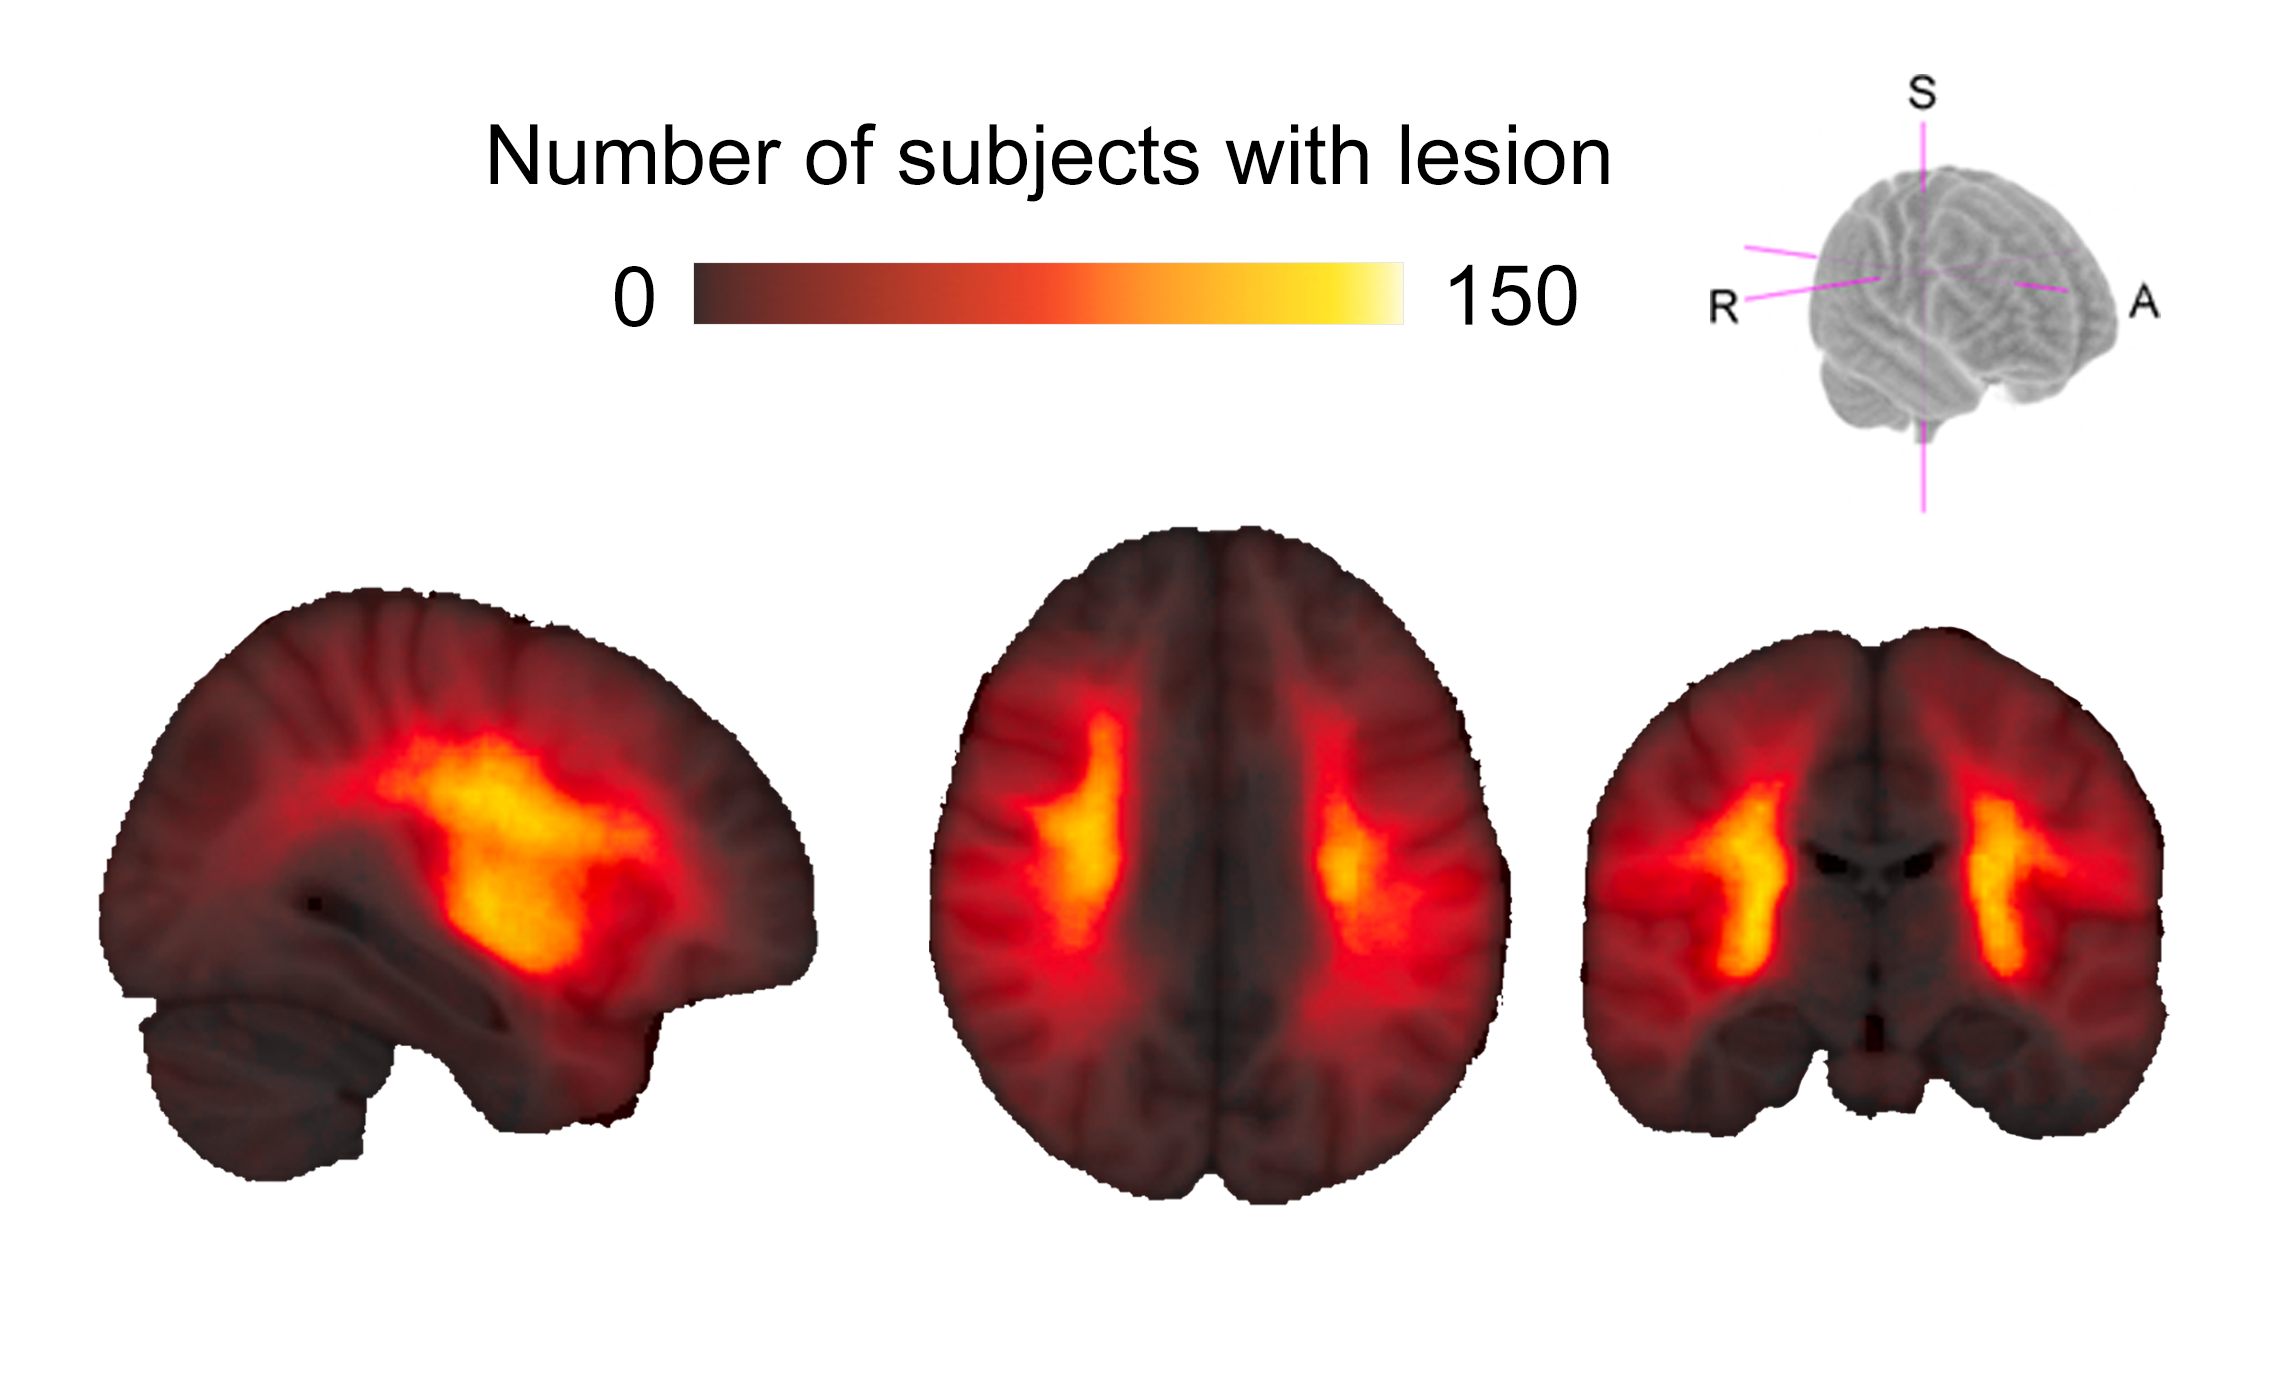
\includegraphics[width=0.8\linewidth]{figures/distribution_lesions.png}
\caption{Distribution of lesions in ENIGMA cohort.}
\label{lesiondist}
\end{figure}


\begin{table}[h]
\centering
\caption{Number of subjects with data for each type of assessment, broken down by chronicity (acute/chronic) and site. FMA UE = Fugl Meyer Assessment of Upper Extremity, Barthel = Barthel Index, NIHSS = National Institutes of Health Stroke Score, ARAT = Action Research Arm Test}
\label{motor_scores}
\begin{tabular}{lrlllllll}
\toprule
 & Total N. & FMA-UE  & Barthel & NIHSS  & ARAT \\
 & & &  &  \\
 \textbf{Acute}  & & & & & \\
\midrule
r005 & 1 & 1 & 0 & 0 & 0 \\
r009 & 50 & 0 & 0 & 50 & 0 \\
r025 & 9 & 9 & 0 & 0 & 0 \\
r028 & 1 & 1 & 0 & 0 & 0 \\
r031 & 36 & 36 & 0 & 0 & 0 \\
r038 & 72 & 0 & 72 & 0 & 0 \\
r040 & 57 & 0 & 57 & 0 & 0 \\
r047 & 2 & 2 & 0 & 0 & 0 \\
r049 & 21 & 0 & 0 & 21 & 0 \\
r050 & 14 & 0 & 0 & 14 & 0 \\
r053 & 52 & 0 & 0 & 52 & 0 \\
r054 & 12 & 12 & 0 & 0 & 0 \\

& & & & & \\
 \textbf{Chronic}  & & & & & \\
\midrule
r001 & 39 & 39 & 0 & 0 & 0 \\
r002 & 12 & 12 & 0 & 0 & 0 \\
r003 & 15 & 15 & 0 & 0 & 0 \\
r004 & 19 & 19 & 0 & 0 & 0 \\
r005 & 27 & 27 & 0 & 0 & 0 \\
r009 & 60 & 0 & 0 & 60 & 0 \\
r025 & 16 & 16 & 0 & 0 & 0 \\
r027 & 28 & 28 & 0 & 0 & 0 \\
r028 & 21 & 21 & 0 & 0 & 0 \\
r031 & 1 & 1 & 0 & 0 & 0 \\
r034 & 15 & 15 & 0 & 0 & 0 \\
r035 & 15 & 15 & 0 & 0 & 0 \\
r038 & 18 & 0 & 18 & 0 & 0 \\
r040 & 14 & 0 & 14 & 0 & 0 \\
r042 & 22 & 22 & 0 & 0 & 0 \\
r044 & 4 & 4 & 0 & 0 & 0 \\
r045 & 4 & 4 & 0 & 0 & 0 \\
r046 & 11 & 11 & 0 & 0 & 0 \\
r047 & 44 & 44 & 0 & 0 & 0 \\
r048 & 43 & 43 & 0 & 0 & 0 \\
r052 & 32 & 32 & 0 & 0 & 0 \\
r053 & 2 & 0 & 0 & 2 & 0 \\
\bottomrule
\end{tabular}
\end{table}


\begin{figure}
\begin{subfigure}{0.5\textwidth}
  \centering
  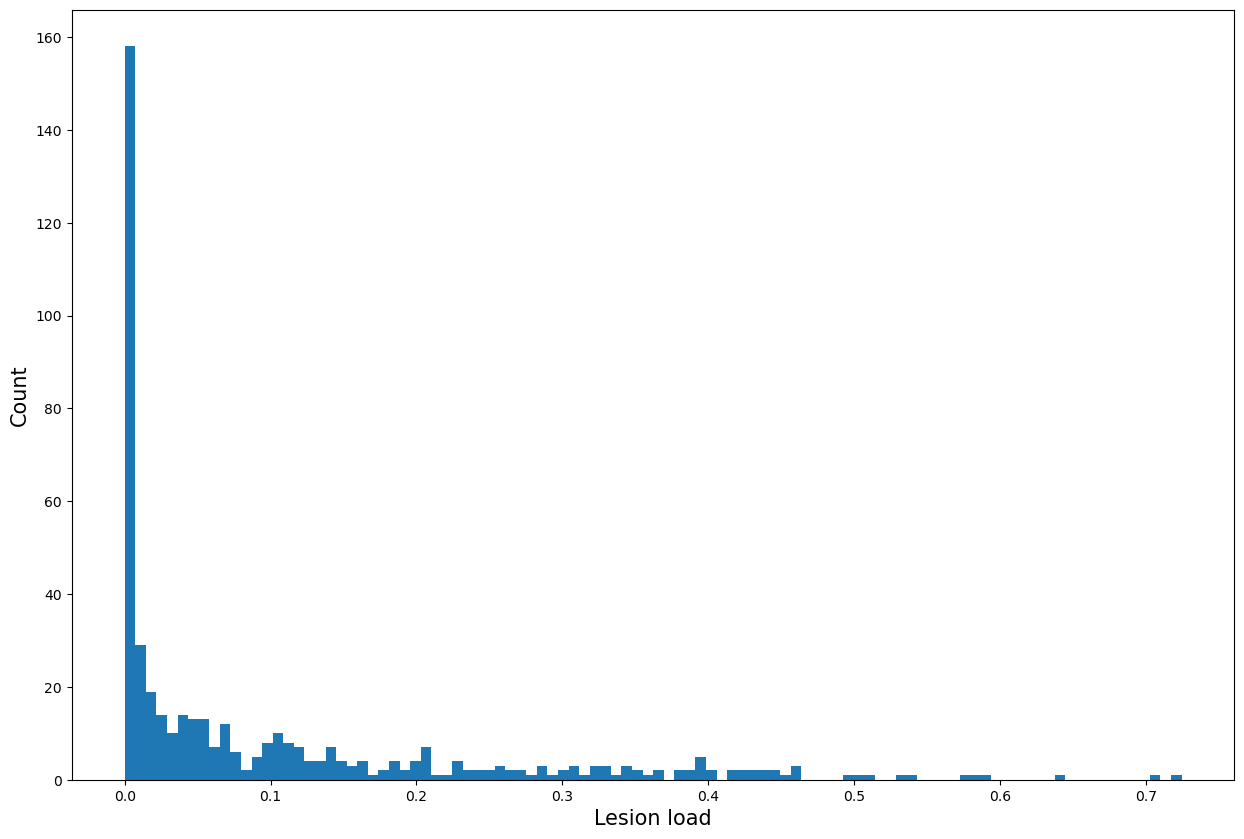
\includegraphics[width=1\linewidth]{figures/m1_lesionload.png}
  \caption{M1-CST lesion load distribution.}
  \label{fig:sfig1}
\end{subfigure}
\begin{subfigure}{0.5\textwidth}
  \centering
  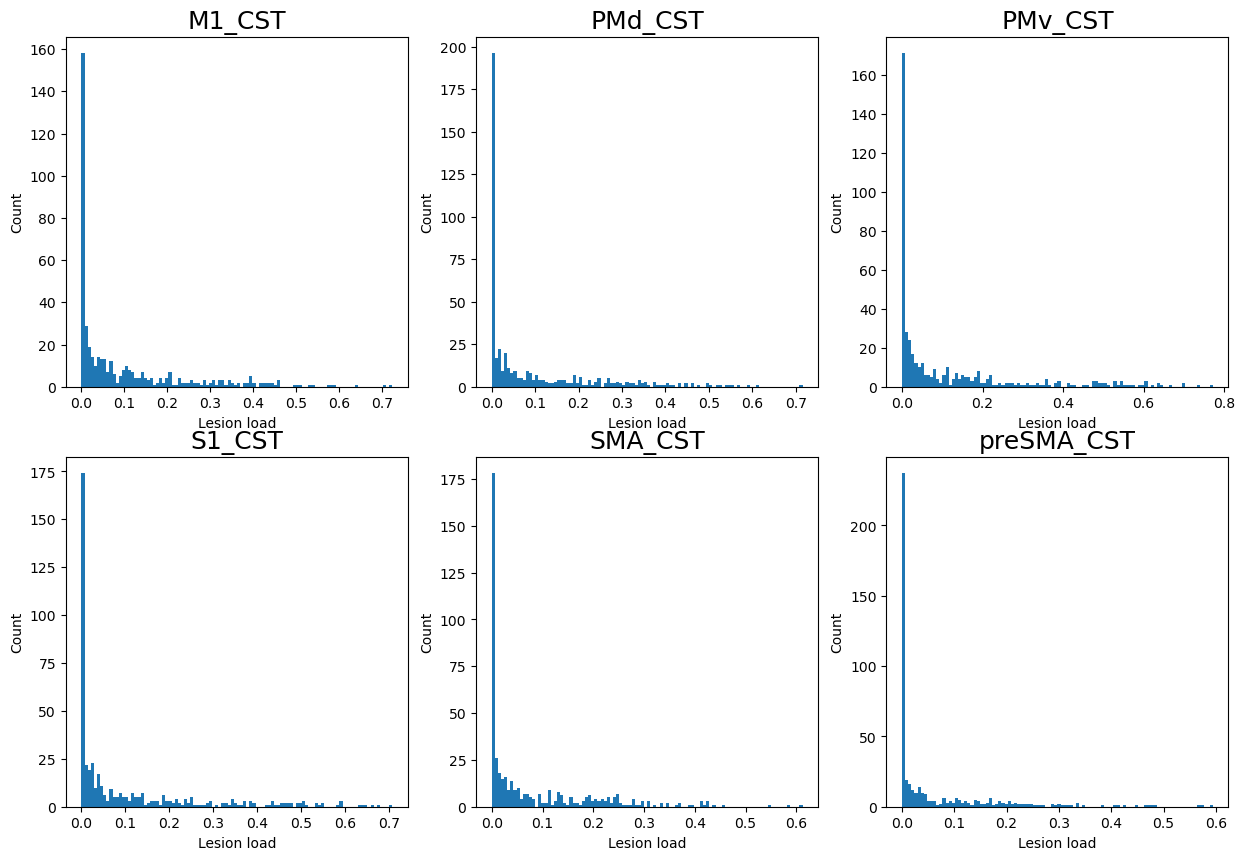
\includegraphics[width=1\linewidth]{figures/all_lesionload.png}
  \caption{Ipsilesional sensorimotor tract template (SMATT) lesion load distribution.}
  \label{fig:sfig2}
\end{subfigure}
\begin{subfigure}{1\textwidth}
  \centering
  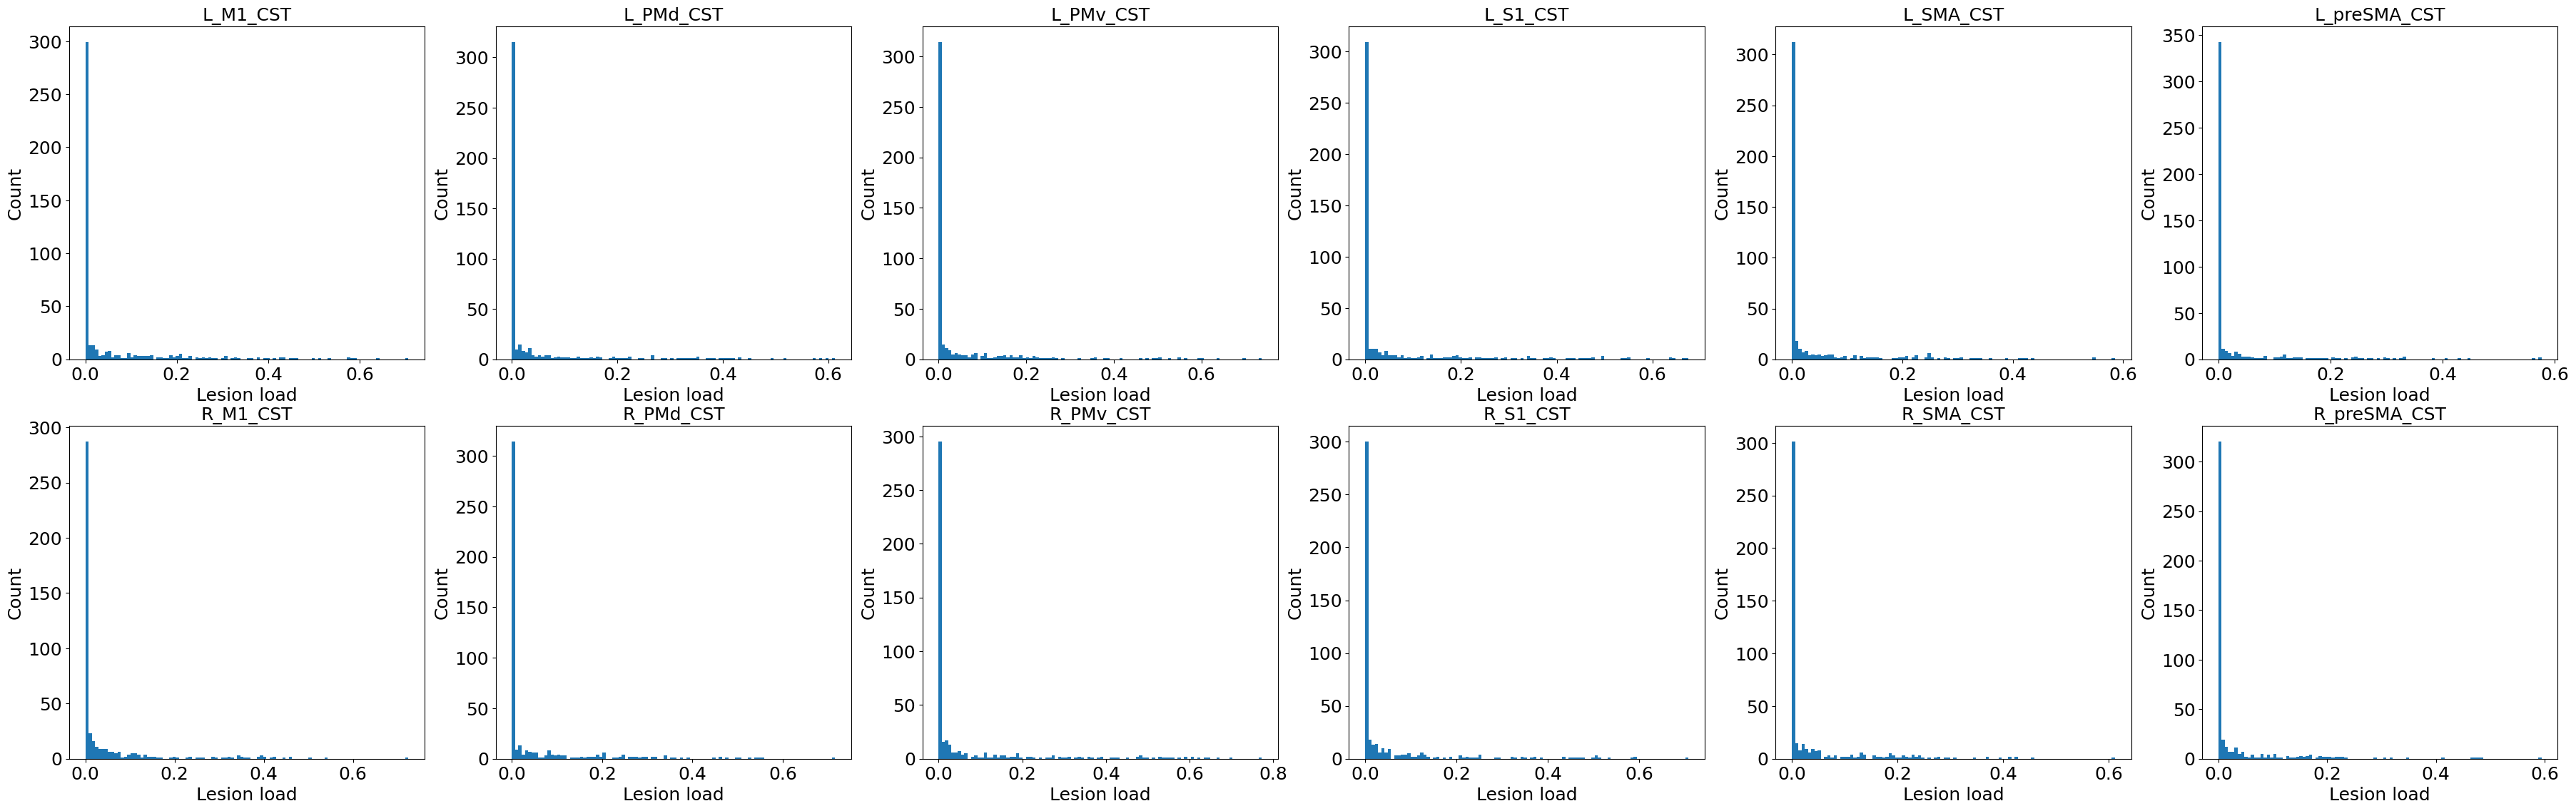
\includegraphics[width=1\linewidth]{figures/all2h_lesionload.png}
  \caption{Left and right hemisphere sensorimotor tract template (SMATT) lesion load distribution.}
  \label{fig:sfig2}
\end{subfigure}
\caption{Distribution of lesion load variables for chronic subjects.}
\label{lesion_load_dist}
\end{figure}


\begin{figure}[ht]
\centering
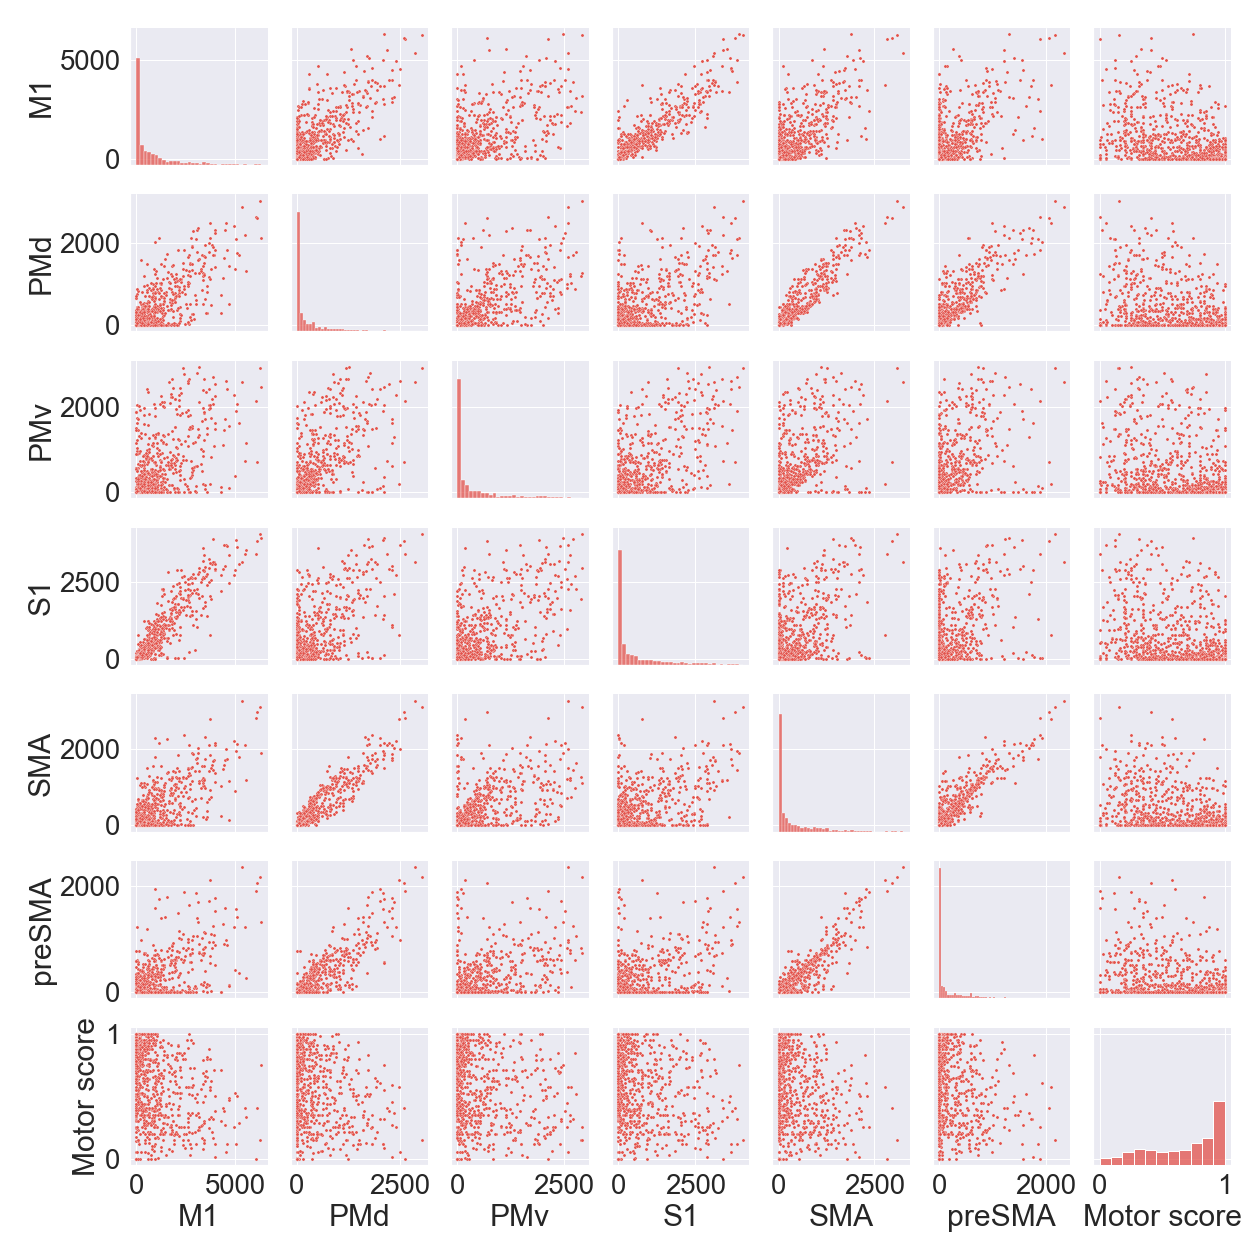
\includegraphics[width=1\linewidth]{figures/SMATT_scatterplts.png}
\caption{Correlations between lesion load calculated for each ipsilesional tract in the sensorimotor area tract template atlas.}
\label{smatt_pairwise_correlations}
\end{figure}

\begin{figure}[ht]
\centering
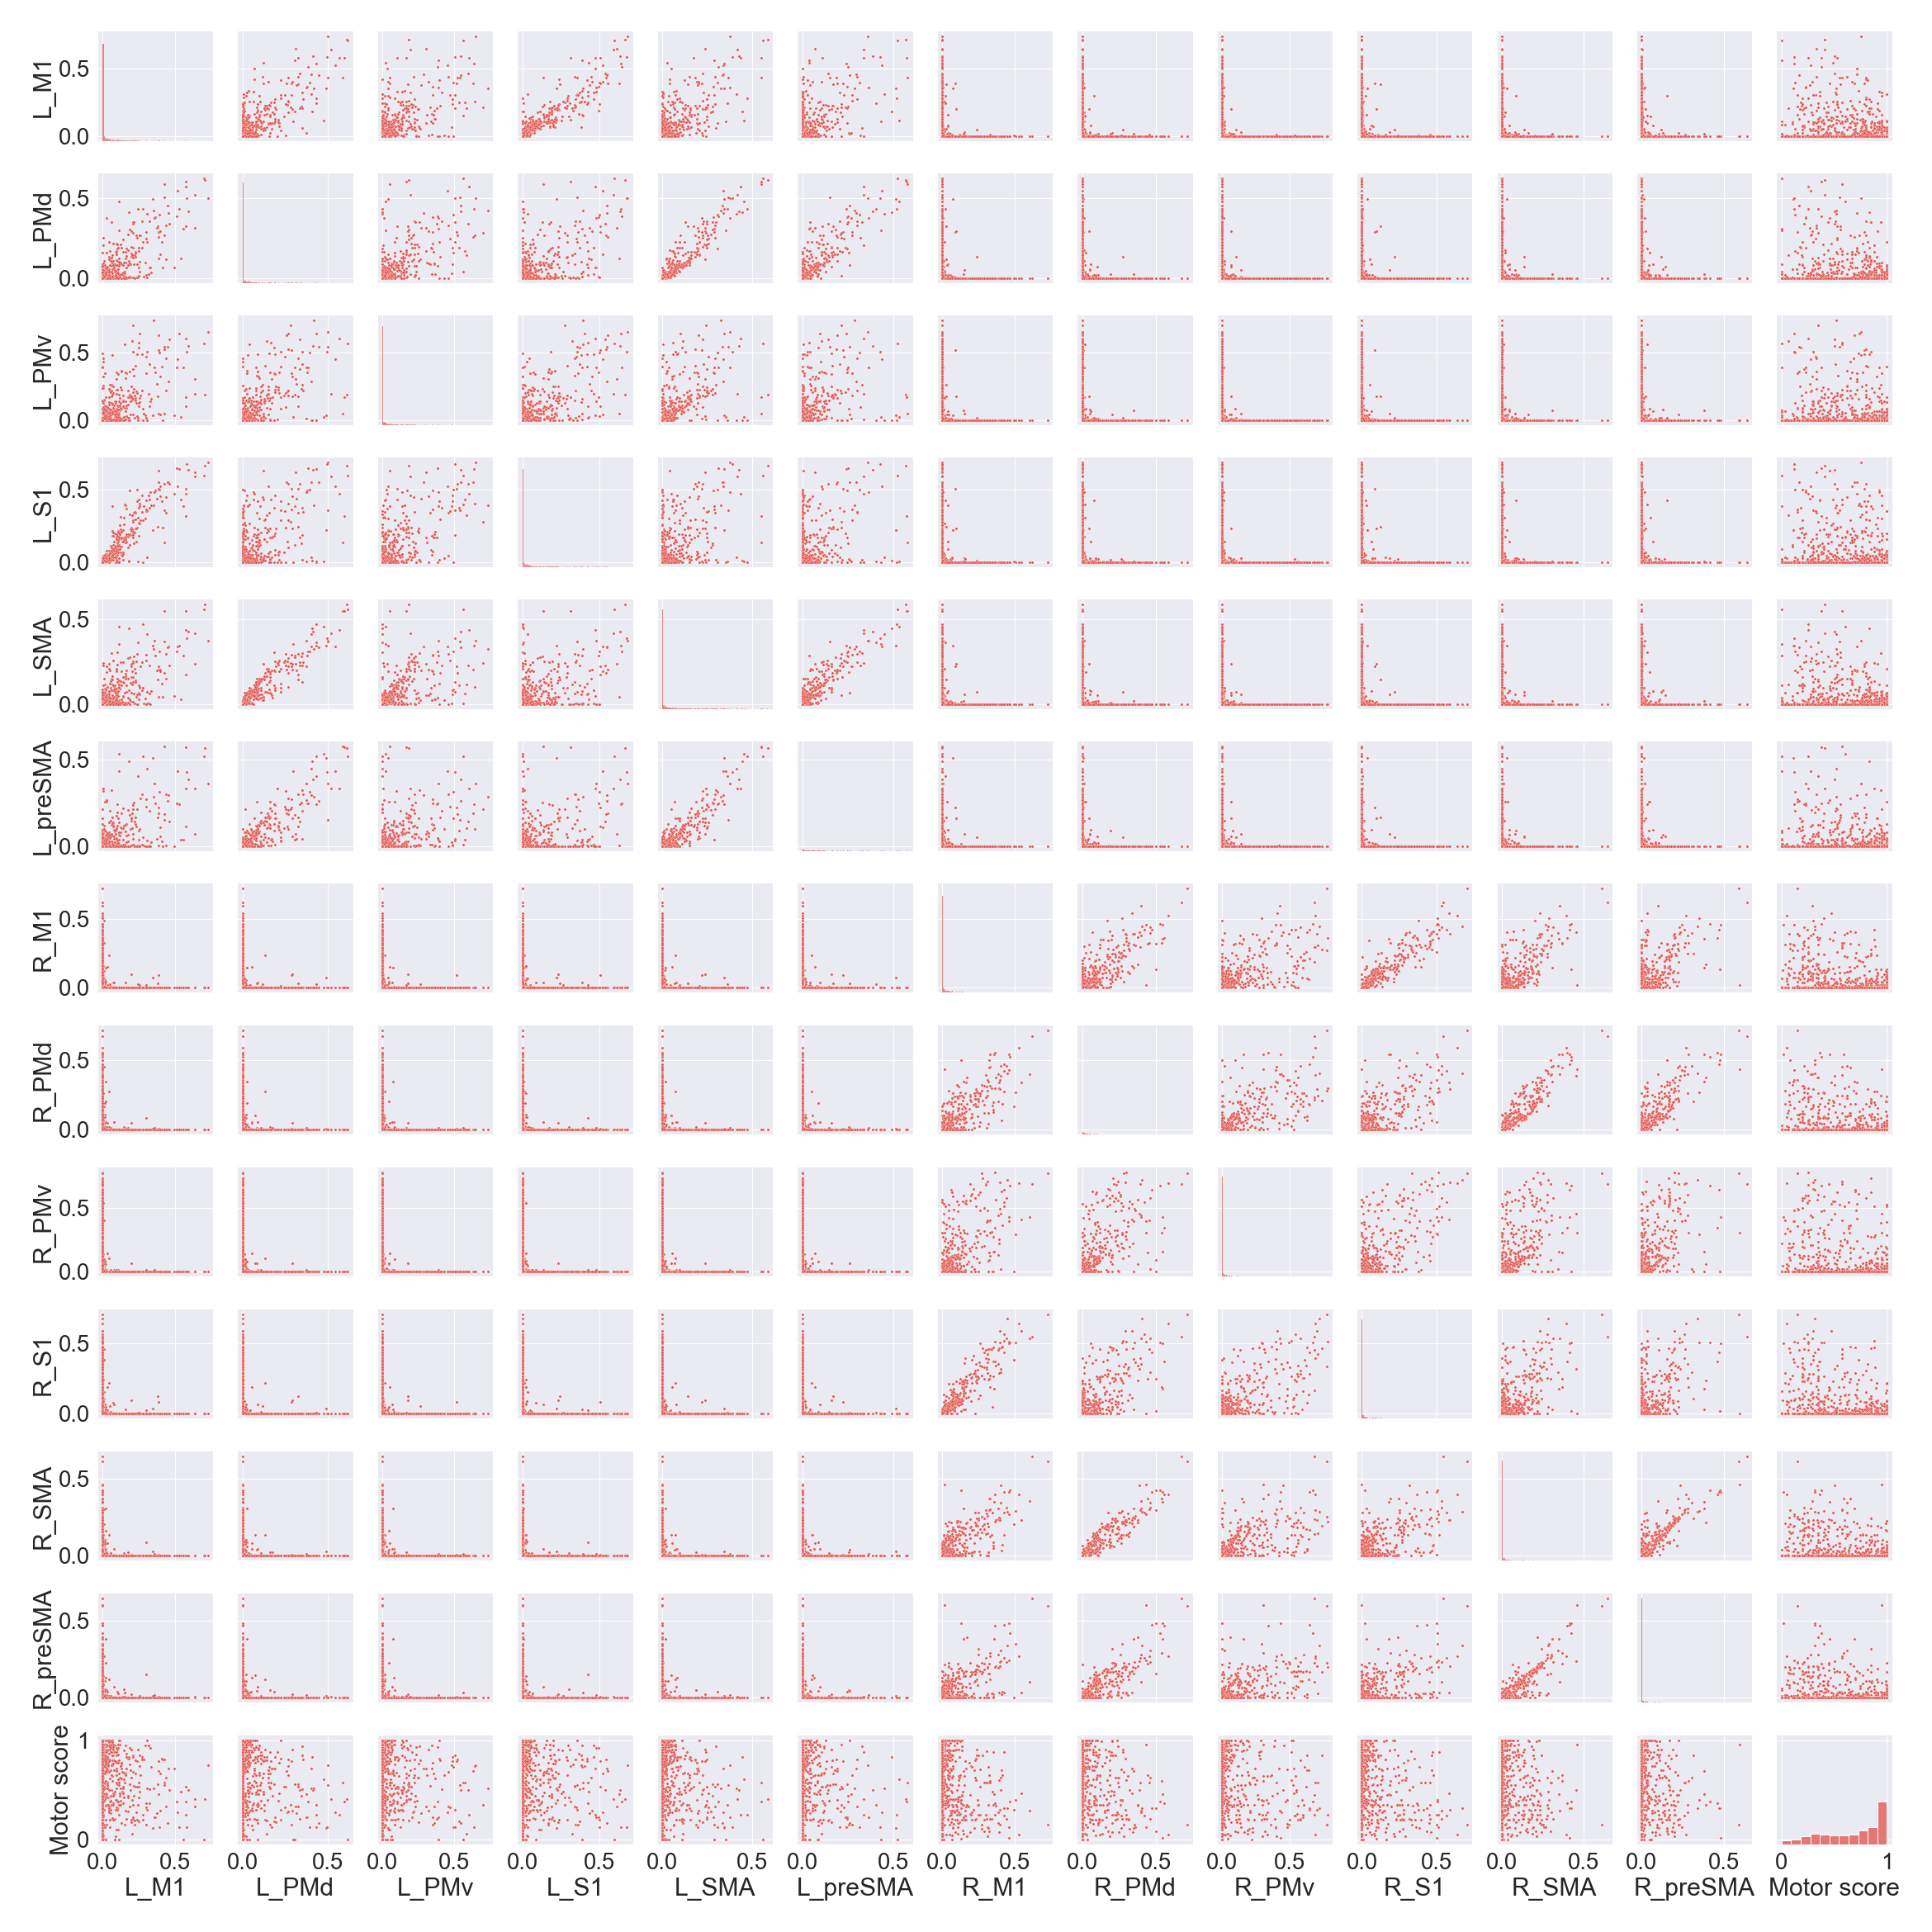
\includegraphics[width=1\linewidth]{figures/SMATT_bi_scatterplts.png}
\caption{Correlations between lesion load calculated for each left and right hemisphere tract in the sensorimotor area tract template atlas.}
\label{smatt_pairwise_correlations_bi}
\end{figure}
\begin{figure}[ht]
\centering
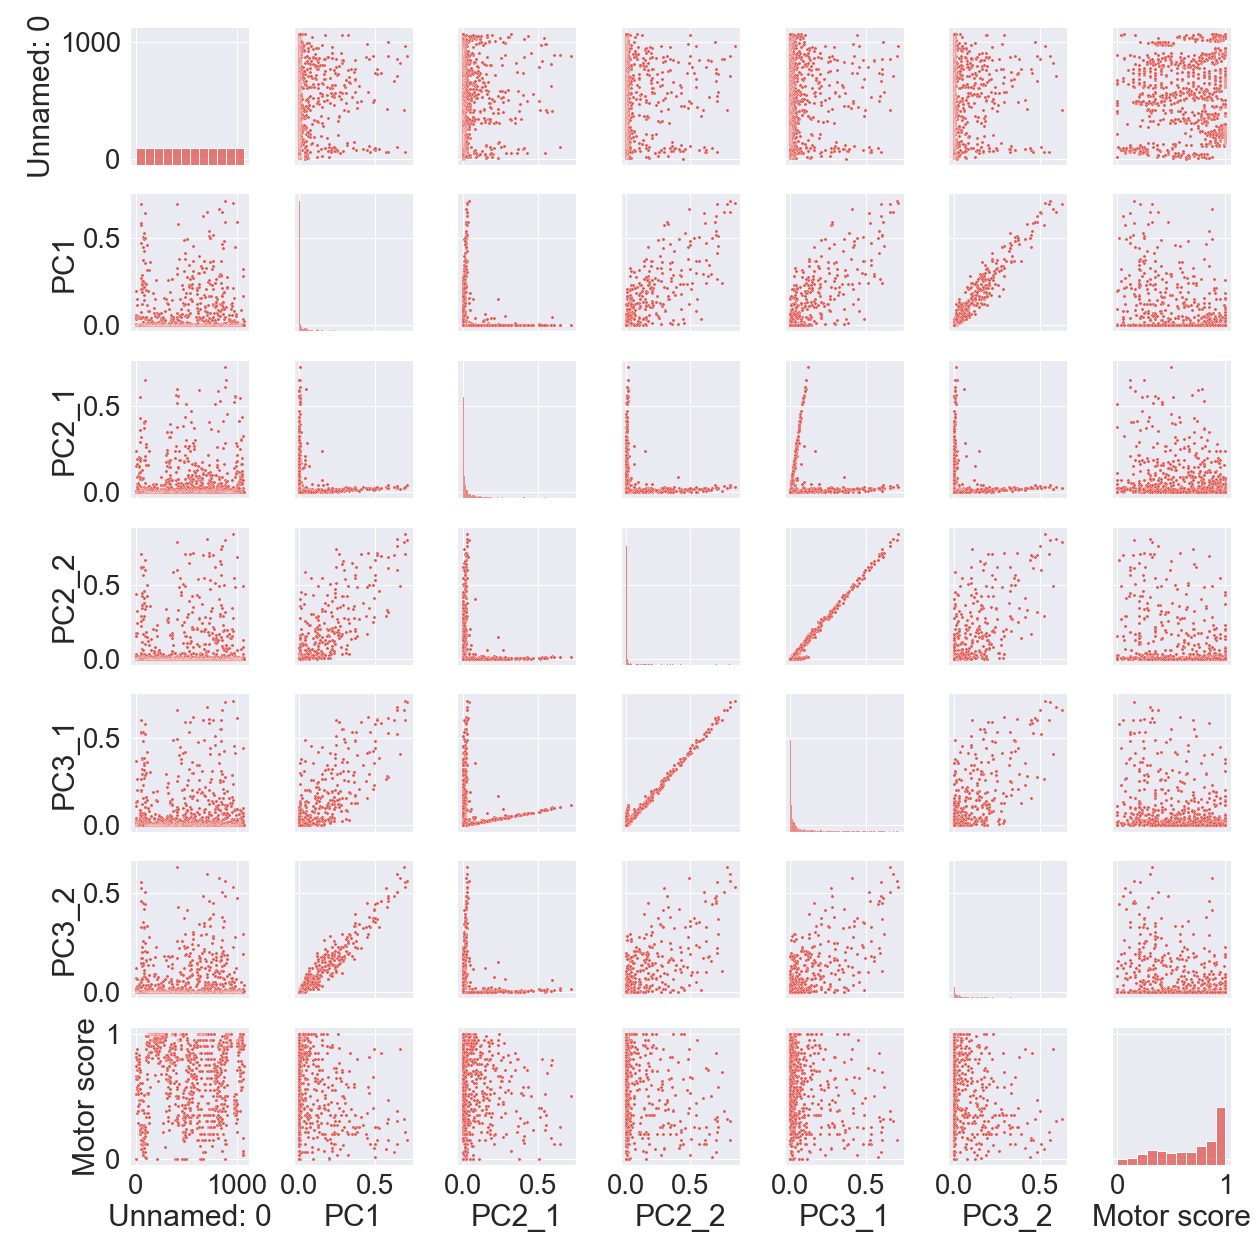
\includegraphics[width=1\linewidth]{figures/slnmvalues_scatterplts.png}
\caption{Correlations between lesion load calculated for each structural lesion network-derived principal component map.}
\label{slnm_distribution}
\end{figure}




\begin{figure}
\begin{subfigure}{1\textwidth}
  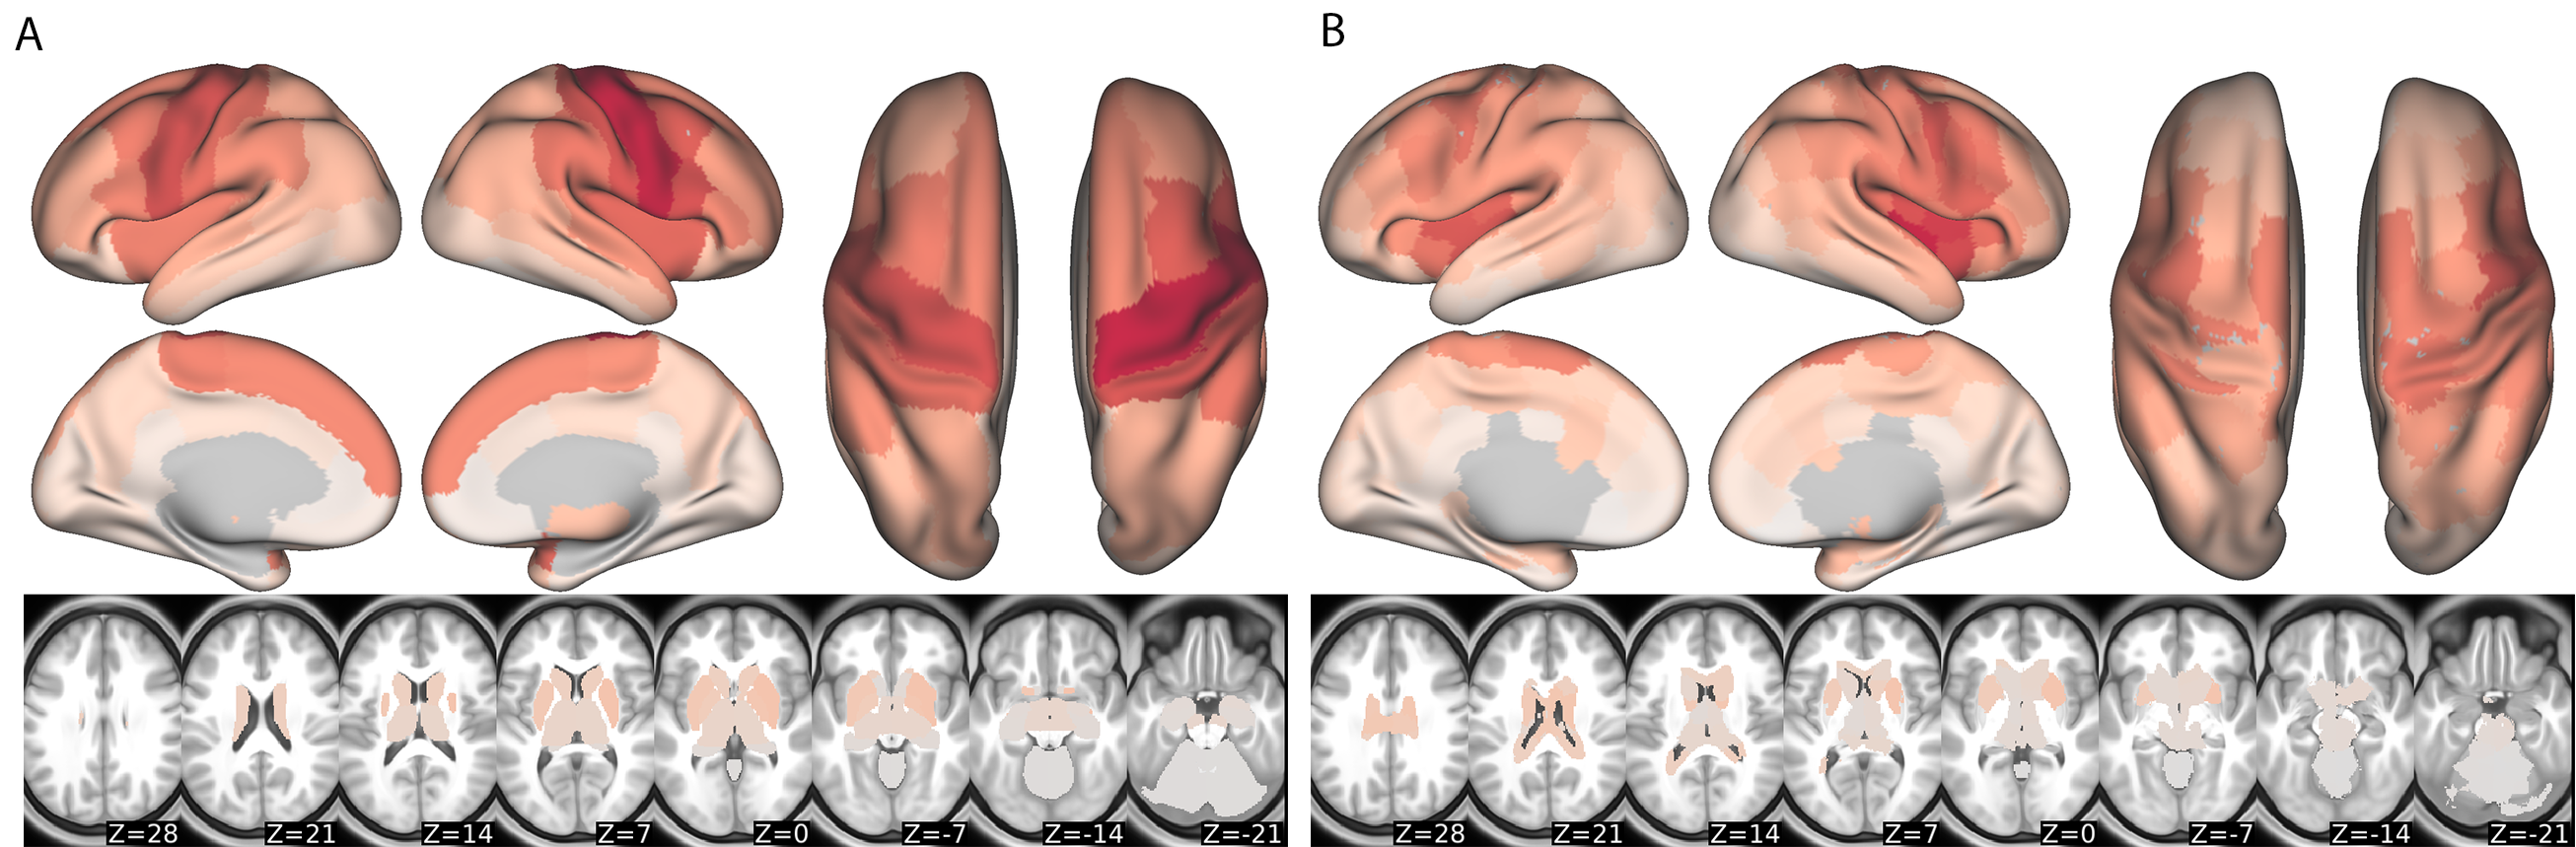
\includegraphics[width=1\linewidth]{figures/mean_chaco.png}
  \caption{Mean regional change in connectivity (ChaCo) scores across acute and chronic subjects used in predictive models. Mean of ChaCo scores parcellated with (\textbf{A}) the FreeSurfer 86-region atlas (min. = 0.005, max. = 0.120) and with (\textbf{B}) the Shen 268-region atlas (min. = 0.0025, max. = 0.146), normalized to the maximum value across regions (red = higher mean ChaCo score across subjects)}
  \label{fig:sfig1}
\end{subfigure}
\begin{subfigure}{1\textwidth}
  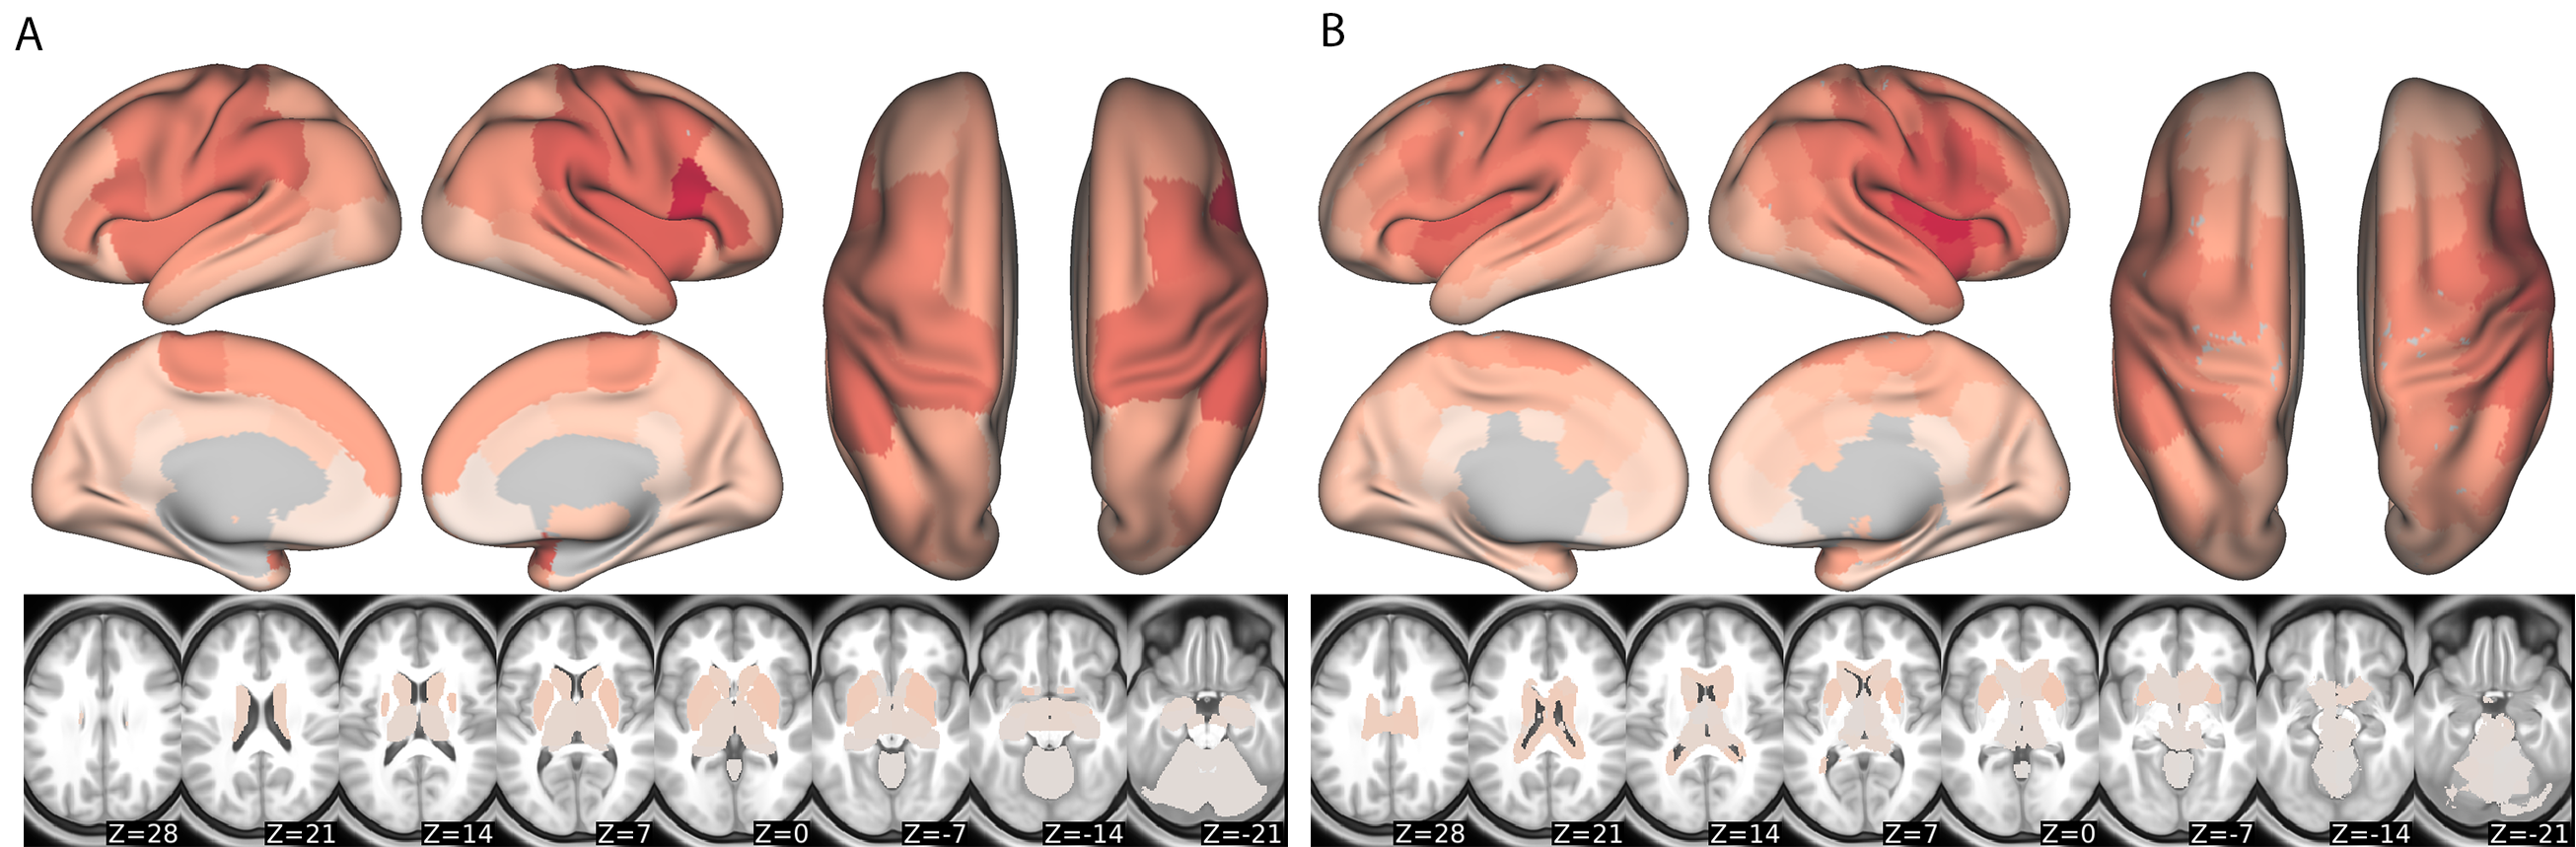
\includegraphics[width=1\linewidth]{figures/std_chaco.png}
  \caption{Standard deviation of regional change in connectivity (ChaCo) scores across acute and chronic subjects used in predictive models. Standard deviation of ChaCo scores parcellated with (\textbf{A}) the FreeSurfer 86-region atlas   (min. = 0.024, max. = 0.26) and with (\textbf{B}) the Shen 268-region atlas (min. = 0.014, max. = 0.29), normalized to the maximum value across regions (red = higher standard deviation of ChaCo score across subjects)} 
  \label{fig:sfig2}
\end{subfigure}
\caption{}
\label{mean_std_chaco}
\end{figure}





\begin{figure}[ht]
\centering
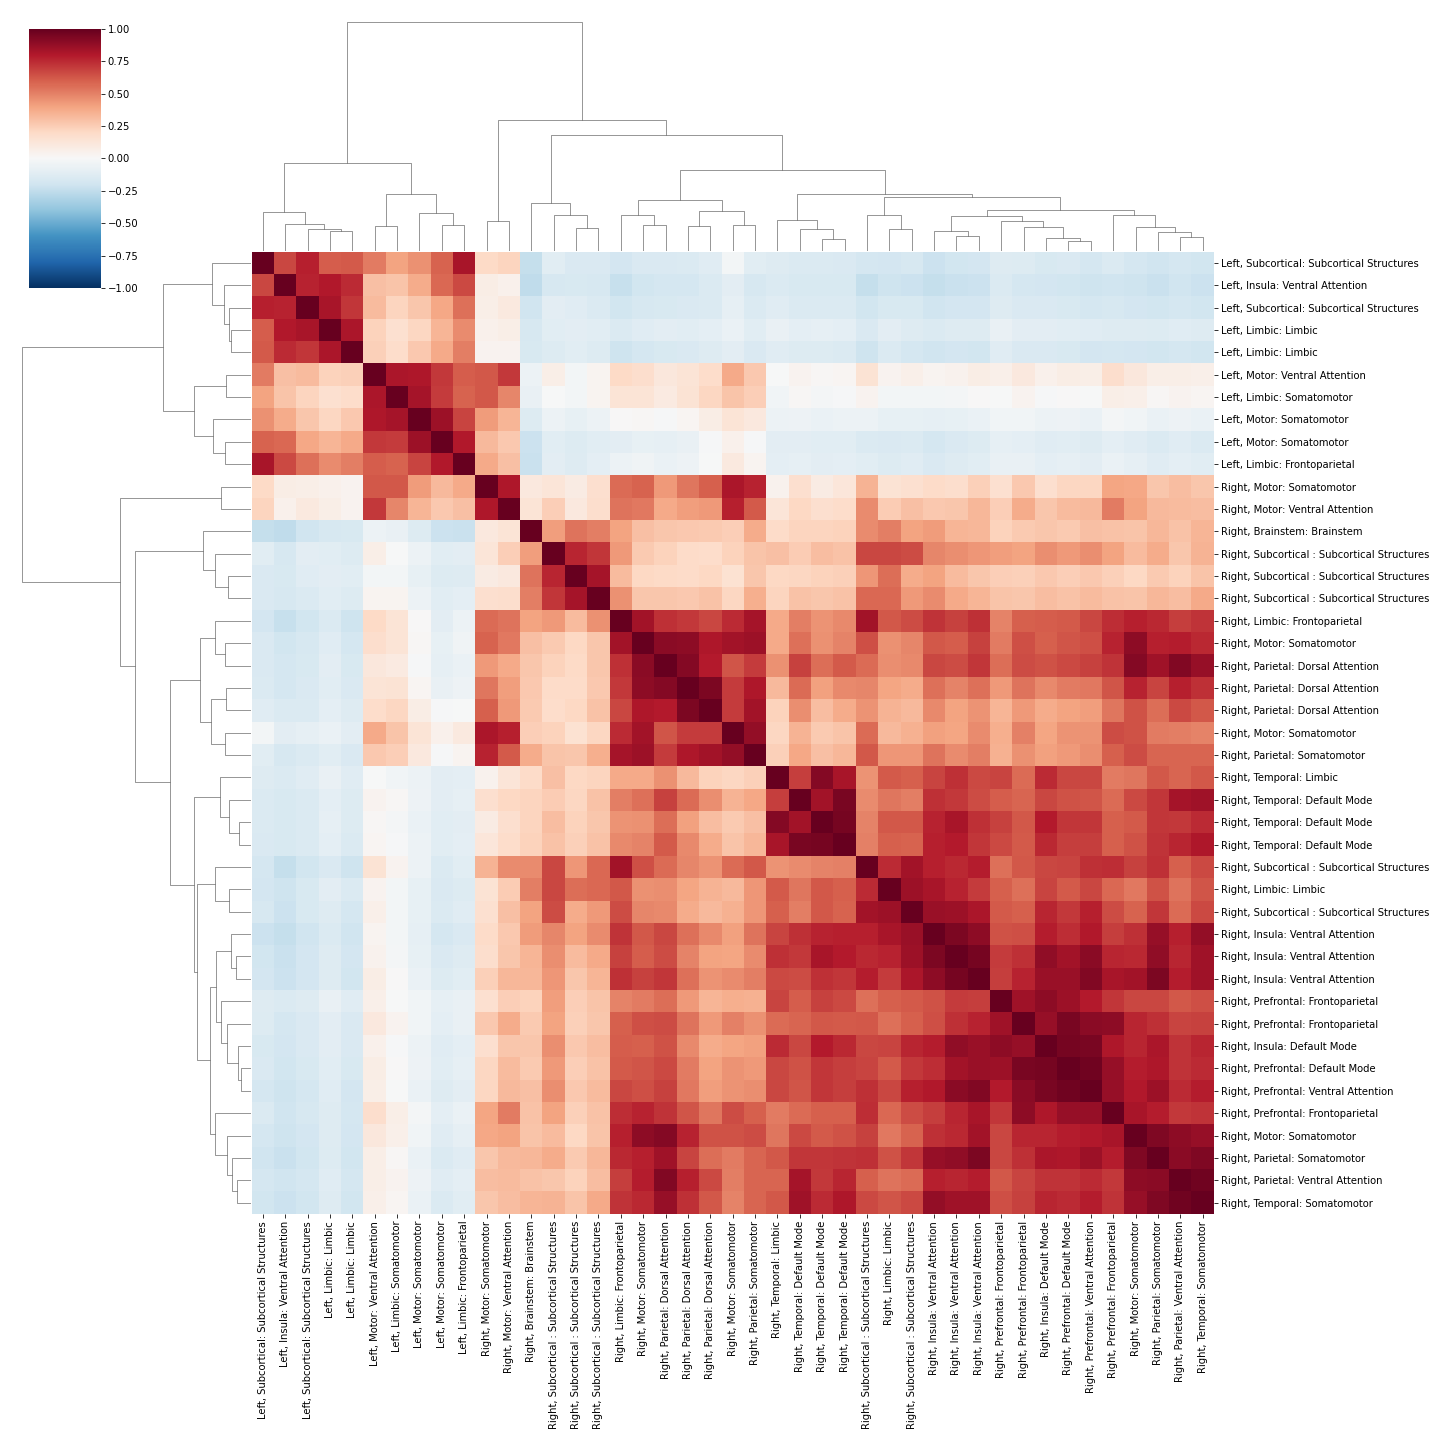
\includegraphics[width=1\linewidth]{figures/heatmap_shen268_correlation_neg.png}
\caption{Hierarchically-clustered heatmap of the correlation matrix of the selected features (ChaCo scores) with negative weights chosen in at least 95 percent of outer folds by correlation-based feature selection in ridge regression using the shen 268-region atlas. Heatmap (top left) displays values corresponding to correlation between features across subjects. Regions are labeled in the following format: "Hemisphere, lobe: Yeo Network".}
\label{heatmap_shen_negweights}
\end{figure}

\begin{figure}[ht]
\centering
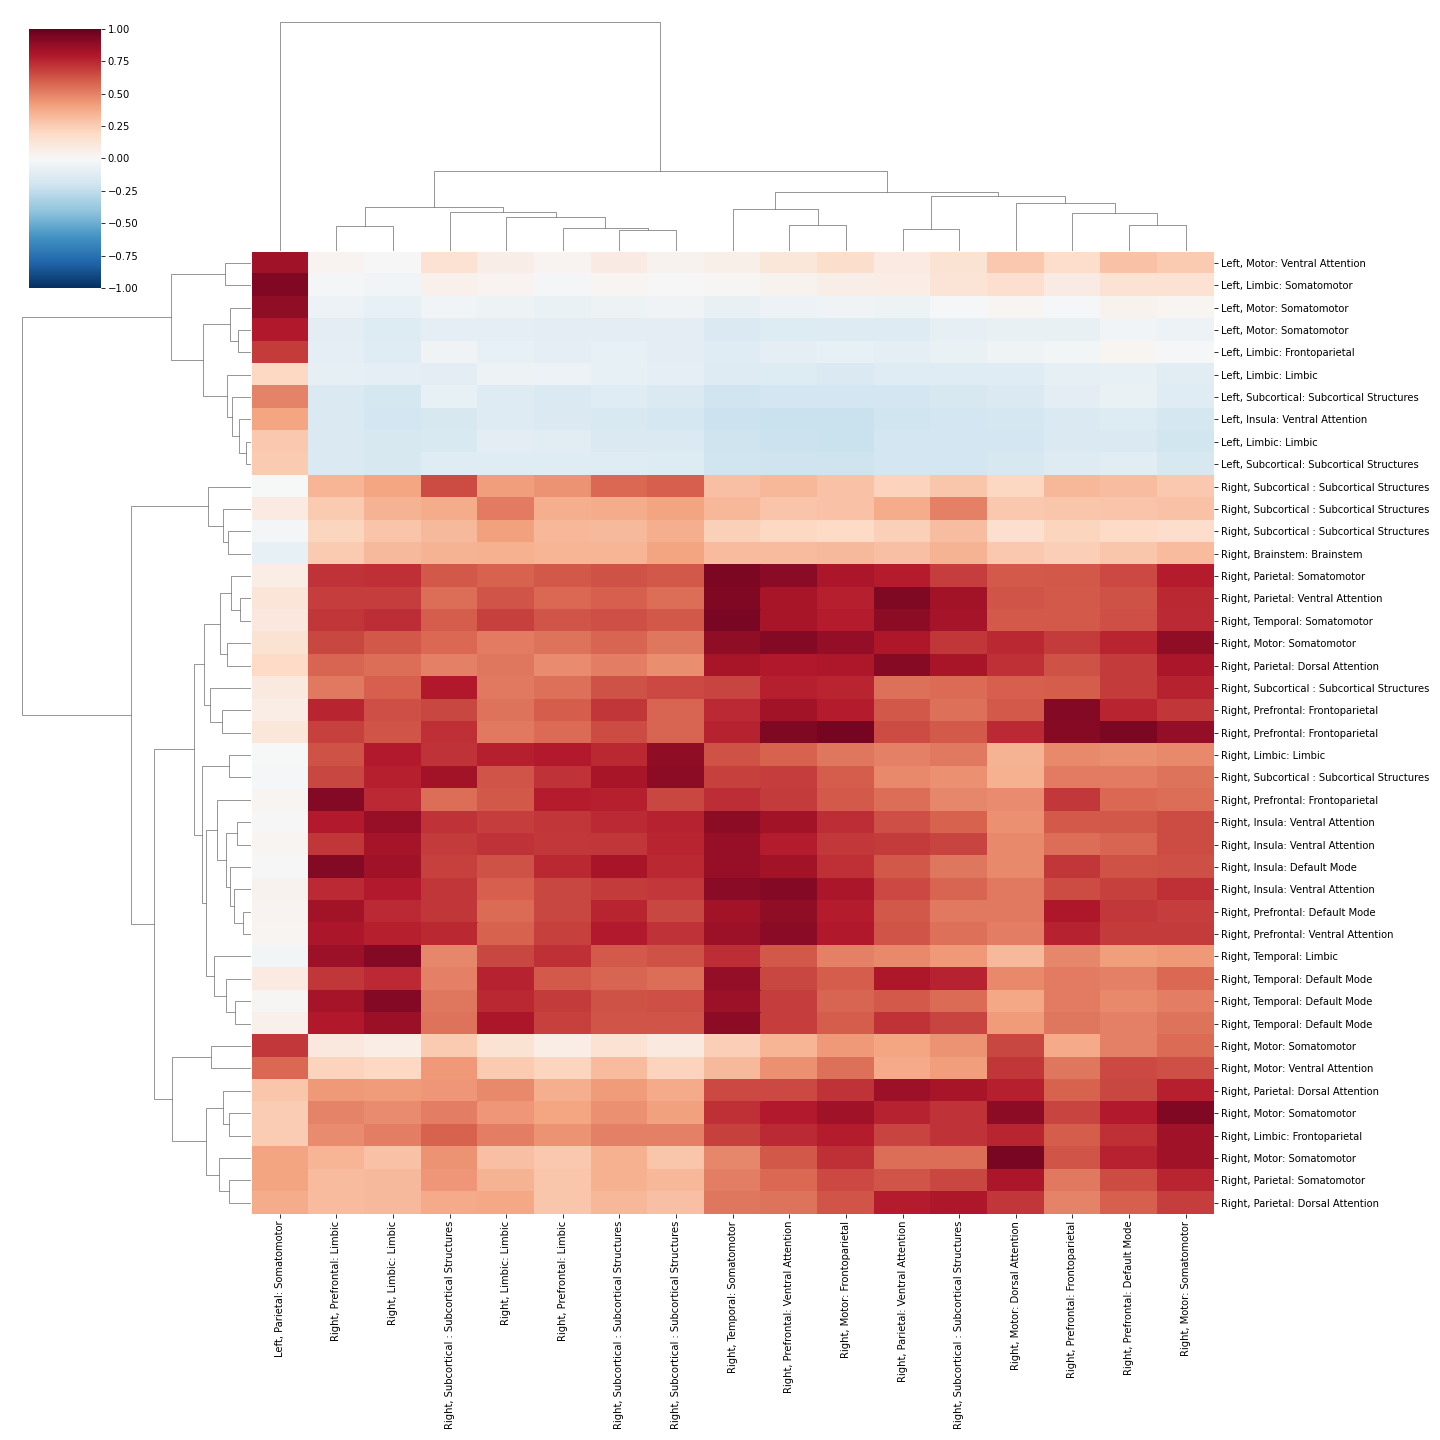
\includegraphics[width=1\linewidth]{figures/heatmap_shen268_correlation_pos_vs_neg.png}
\caption{Hierarchically-clustered heatmap of the correlation matrix of all selected features, split by negative and positive regression weights. Vertical (right) axis: regions with negative weights, horizontal (bottom) axis: regions with positive weights.  Regions are labeled in the following format: "Hemisphere, lobe: Yeo Network".}
\label{heatmap_shen_pos_vs_negative}
\end{figure}


\begin{figure}
\begin{subfigure}{0.5\textwidth}
  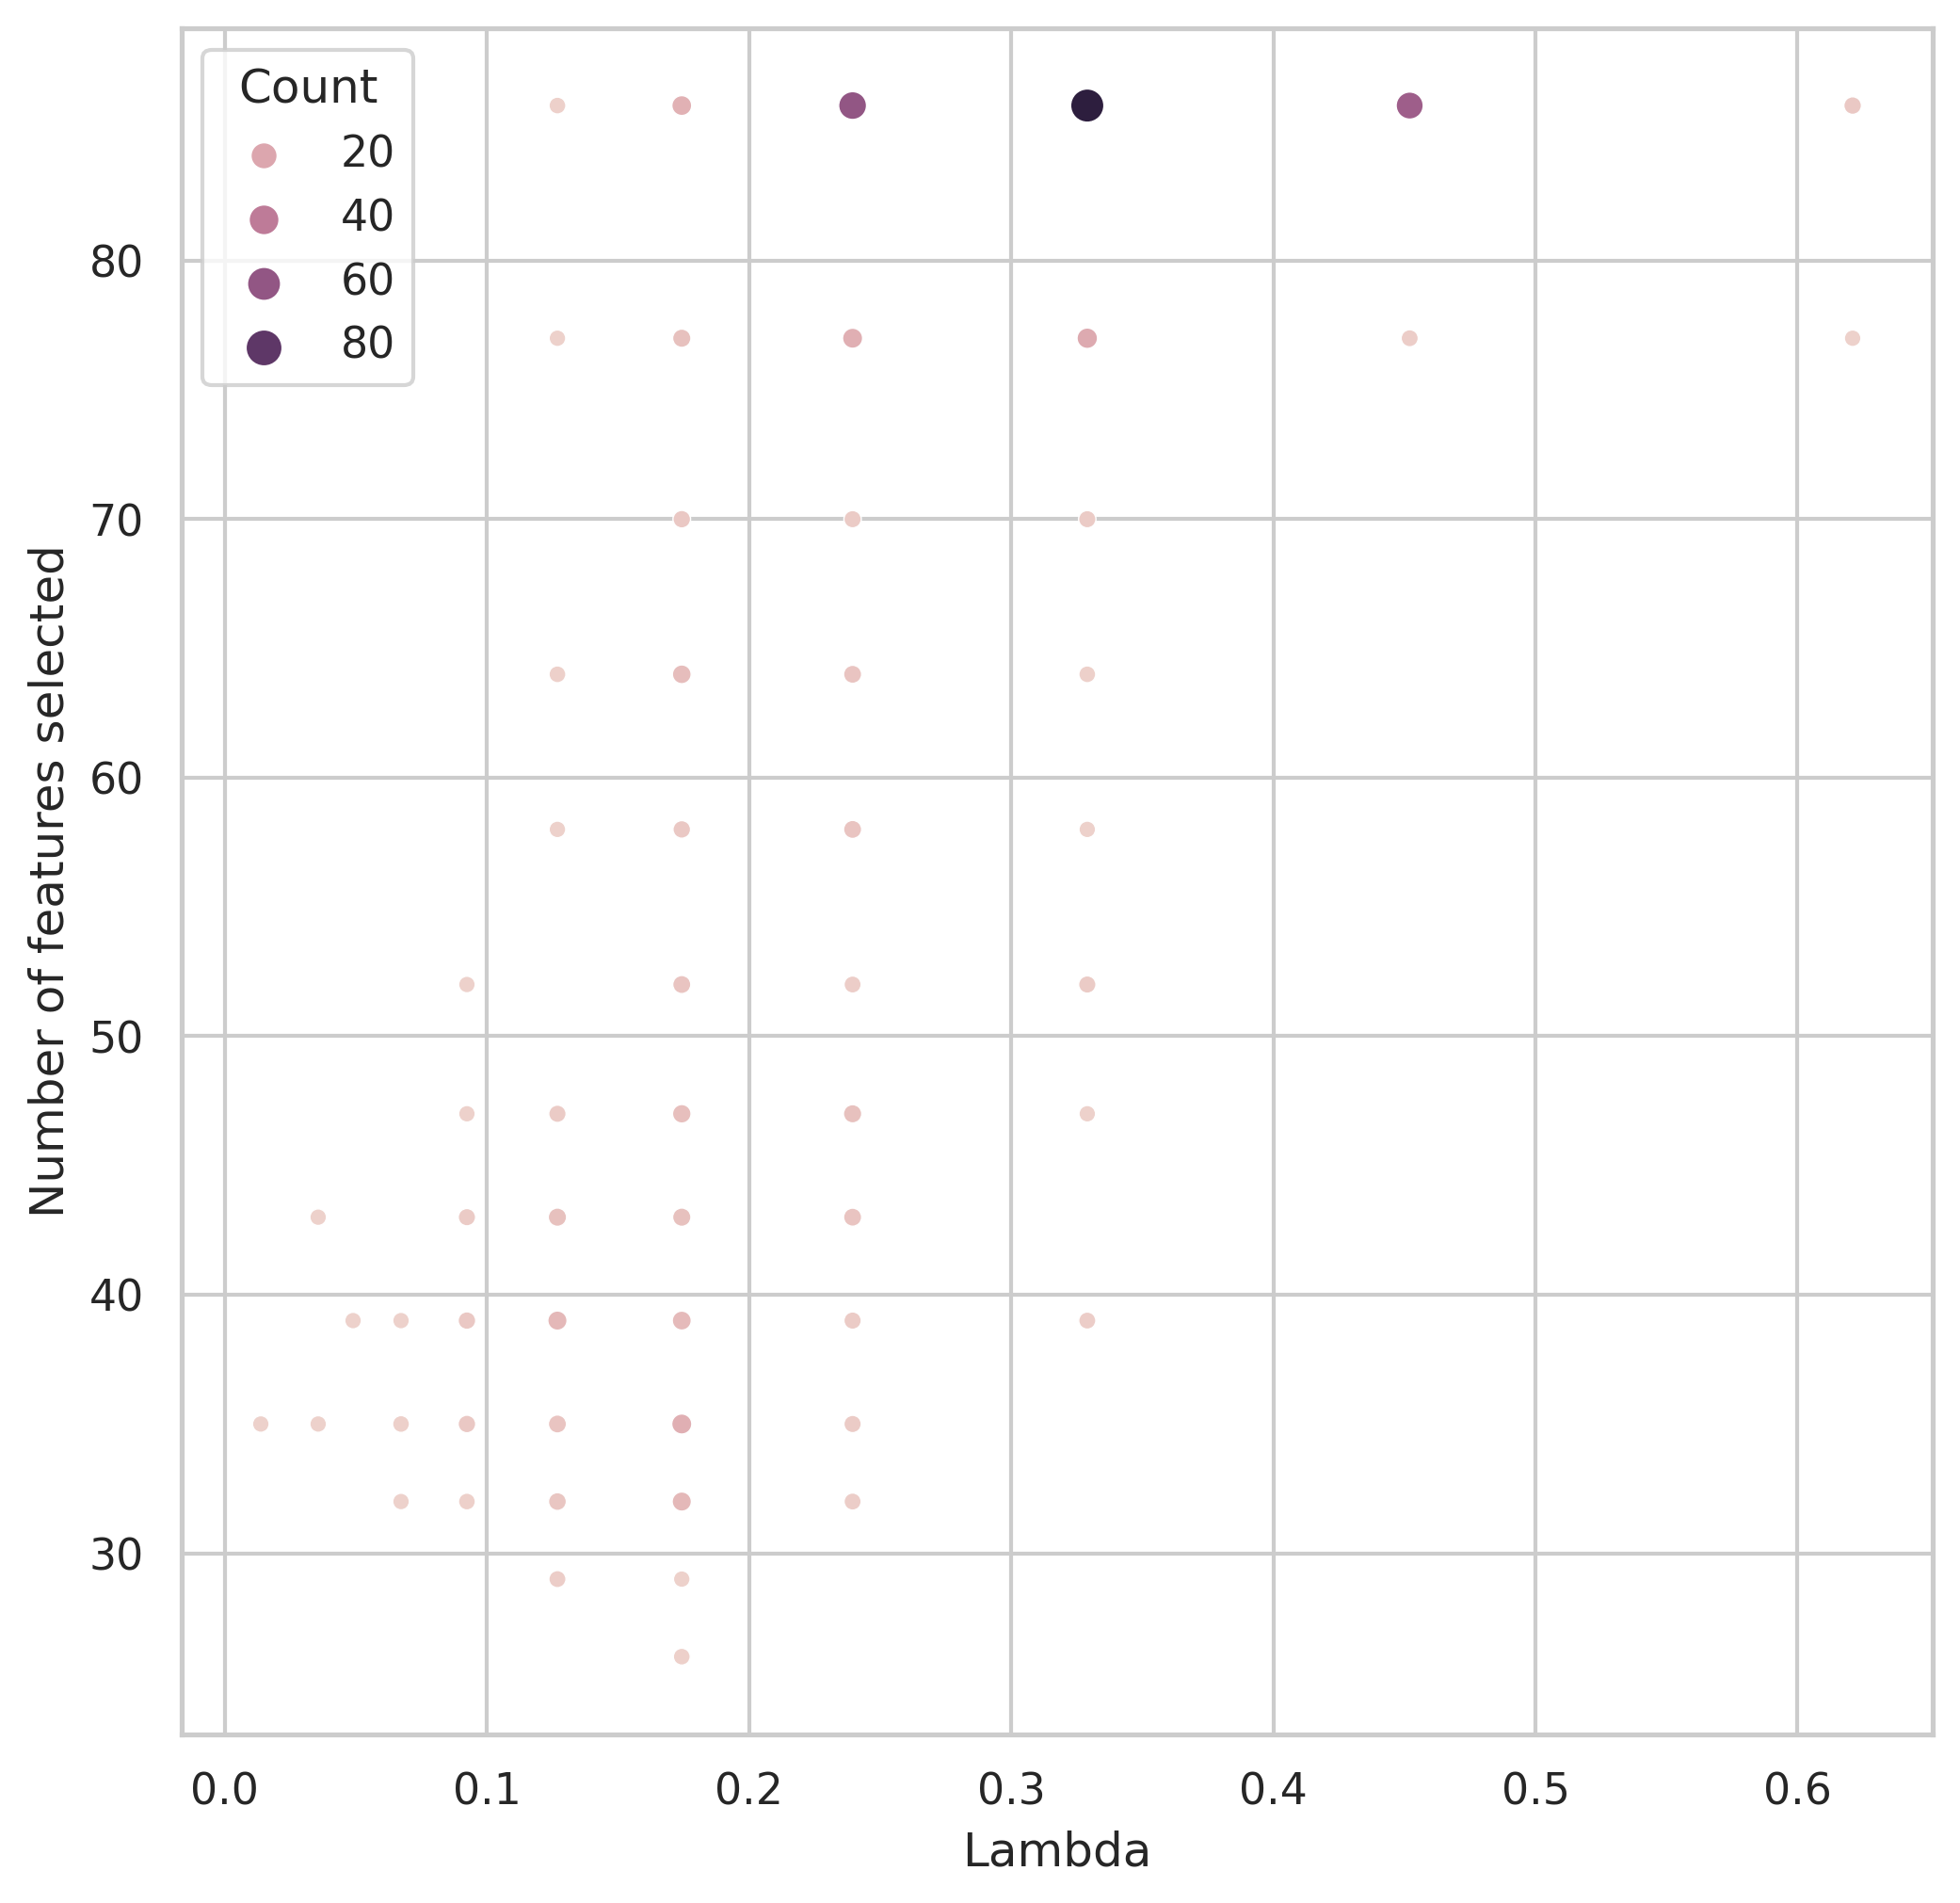
\includegraphics[width=1\linewidth]{figures/fs86subj_normed_motor_scores_chacovol_acutechronic_ridge_crossval1nfeats_lambdas.png}
  \caption{Number of features selected vs. lambda (amount of regularization) for model using ChaCo scores with the FreeSurfer 86-region atlas, acute and chronic subjects together in the training dataset, predicting noromed motor scores. Distribution is showing all training folds (i.e. 500 training folds, 5 folds x 100 permutations)}
  \label{fig:sfig1}
\end{subfigure}
\begin{subfigure}{0.5\textwidth}
  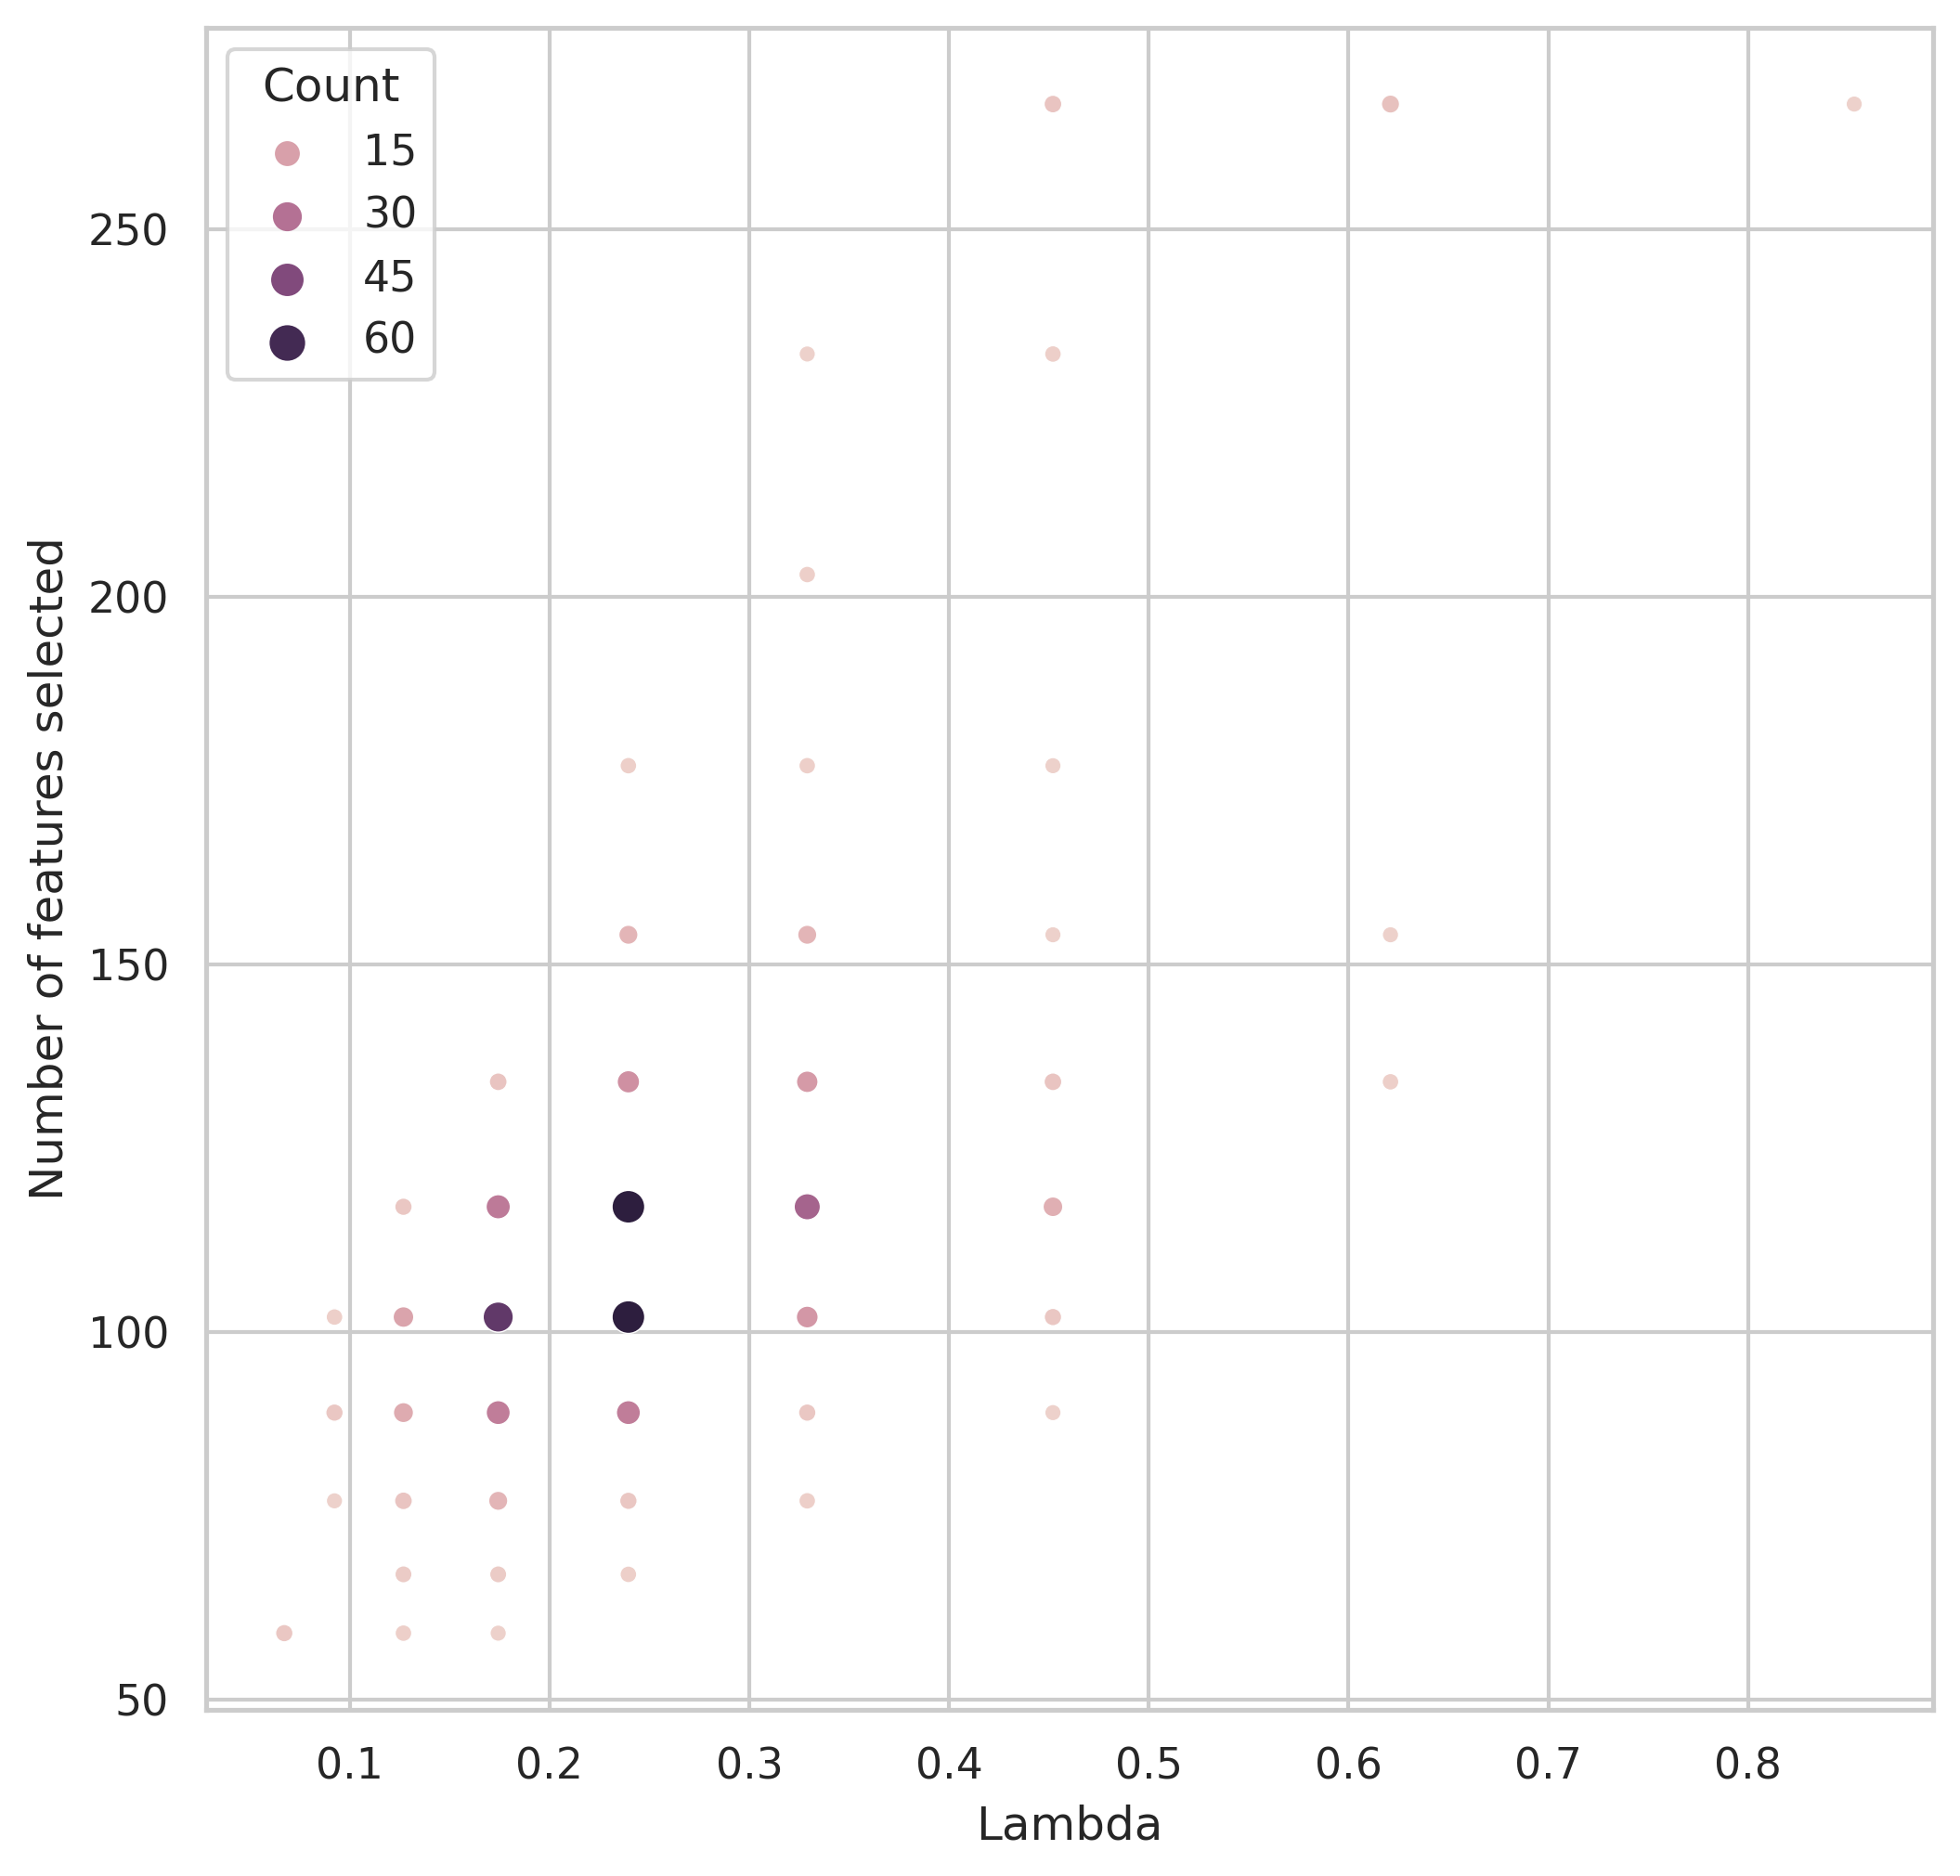
\includegraphics[width=1\linewidth]{figures/shen268_normed_motor_scores_chacovol_acutechronic_ridge_crossval1nfeats_lambdas.png}
  \caption{Number of features selected vs. lambda (amount of regularization) for model using ChaCo scores with the Shen 268-region atlas, acute and chronic subjects together in the training dataset, predicting normed motor scores.Distribution is showing all outer folds (i.e. 500 outer folds, 5 folds x 100 permutations)} 
  \label{fig:sfig2}
\end{subfigure}
\caption{Distribution of number of features selected in ChaCo models (fs86 left, shen268 right) vs. amount of regularization.}
\label{lambda_kappa}
\end{figure}


\begin{figure}[htp]
\centering
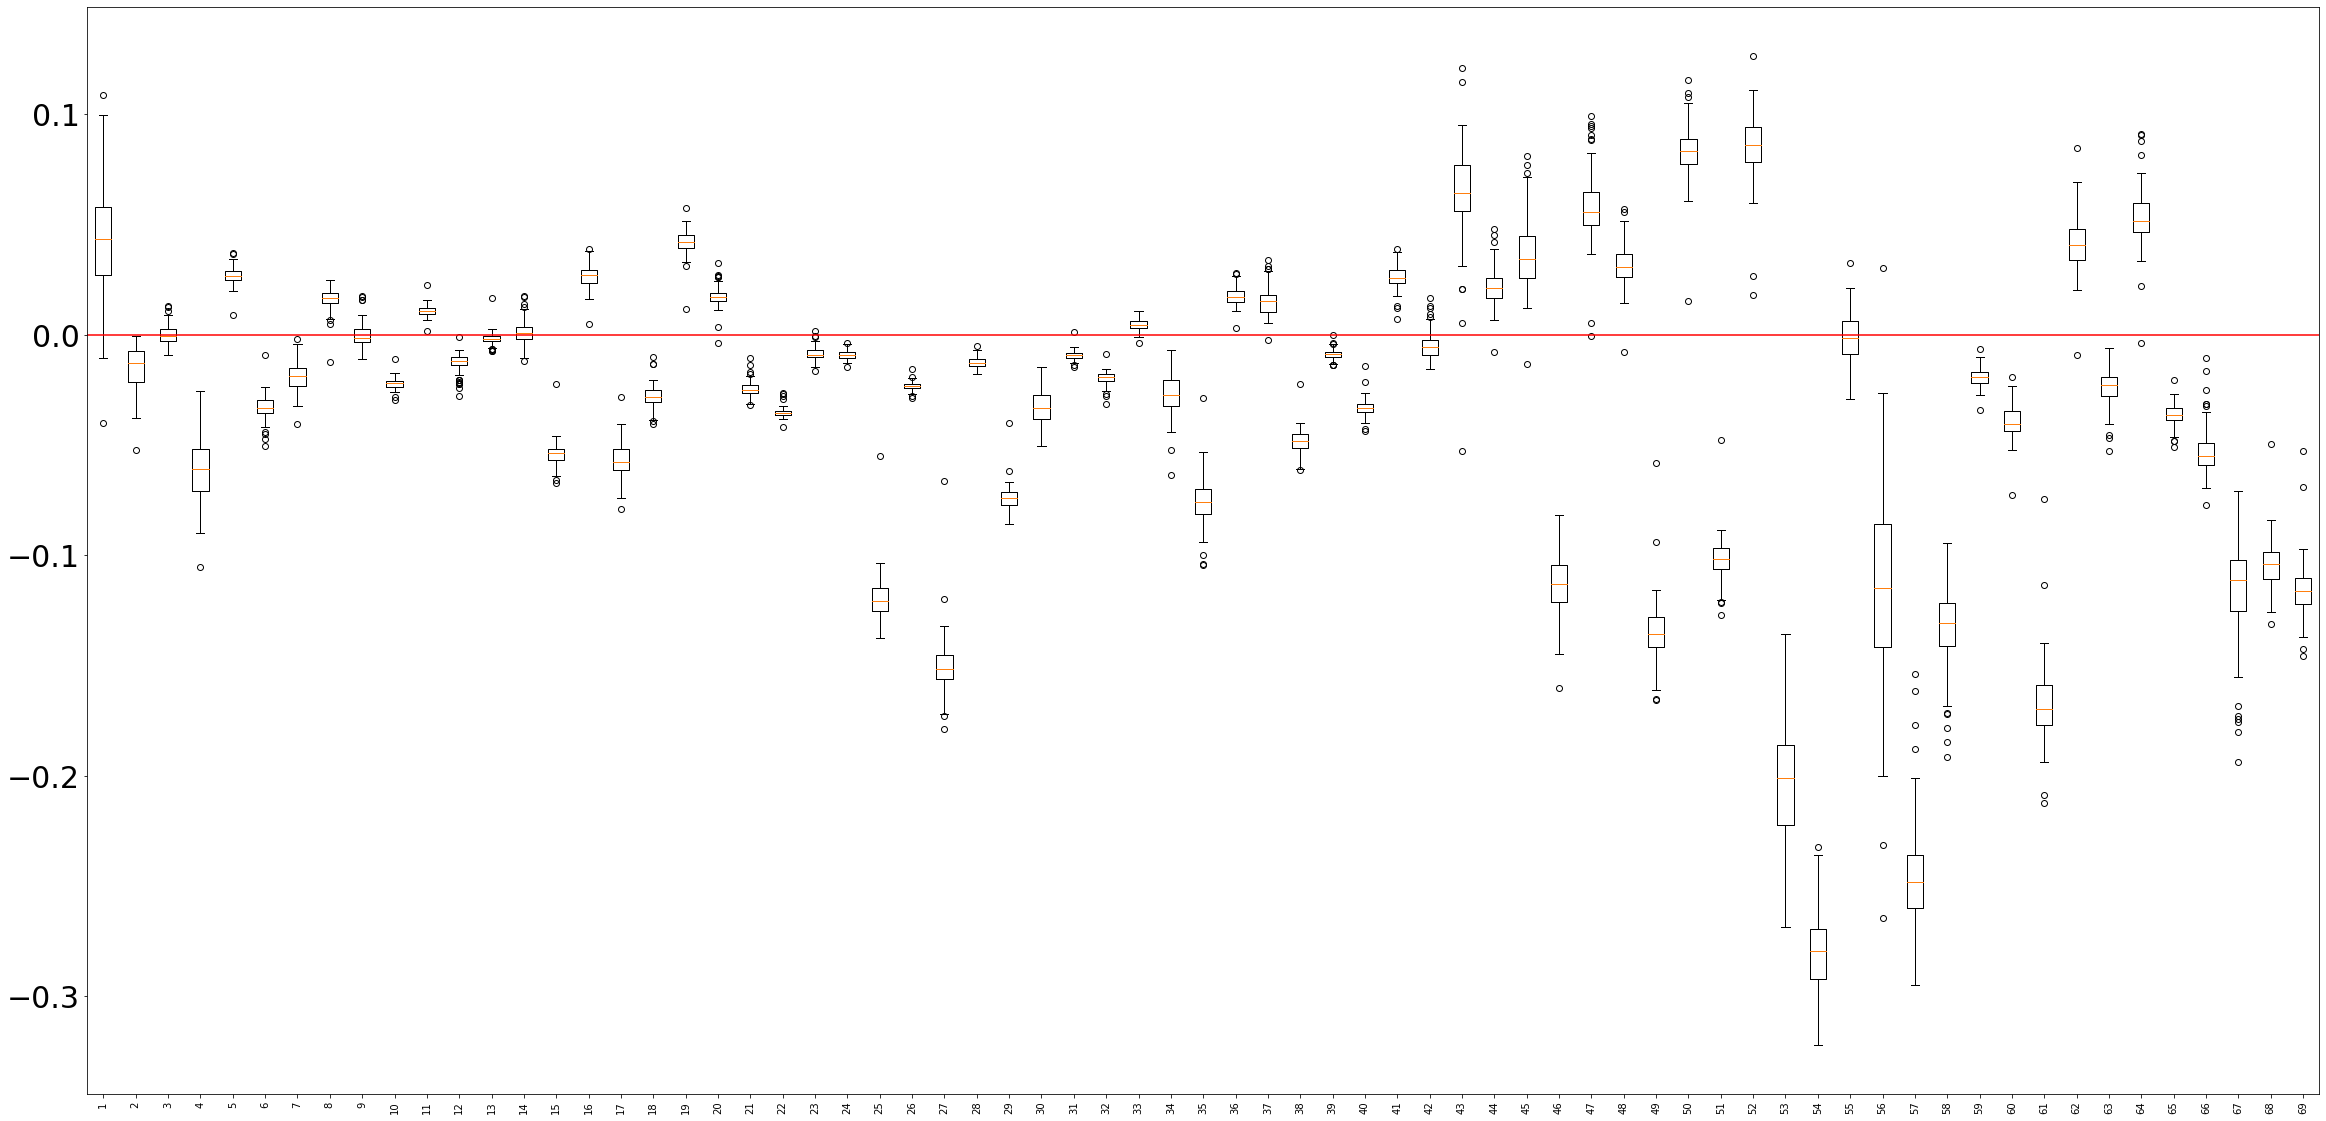
\includegraphics[width=1\linewidth]{figures/distribution_mean_beta_only_top95.png}
\caption{Distribution of mean (average over 5 folds) beta coefficients for features that were selected in at least 475/500 outer folds for Shen268-ChaCo models. Regions are listed on the x-axis and beta values on the y-axis.}
\label{shen_beta_coeffs}
\end{figure}


\begin{figure}[htp]
\centering
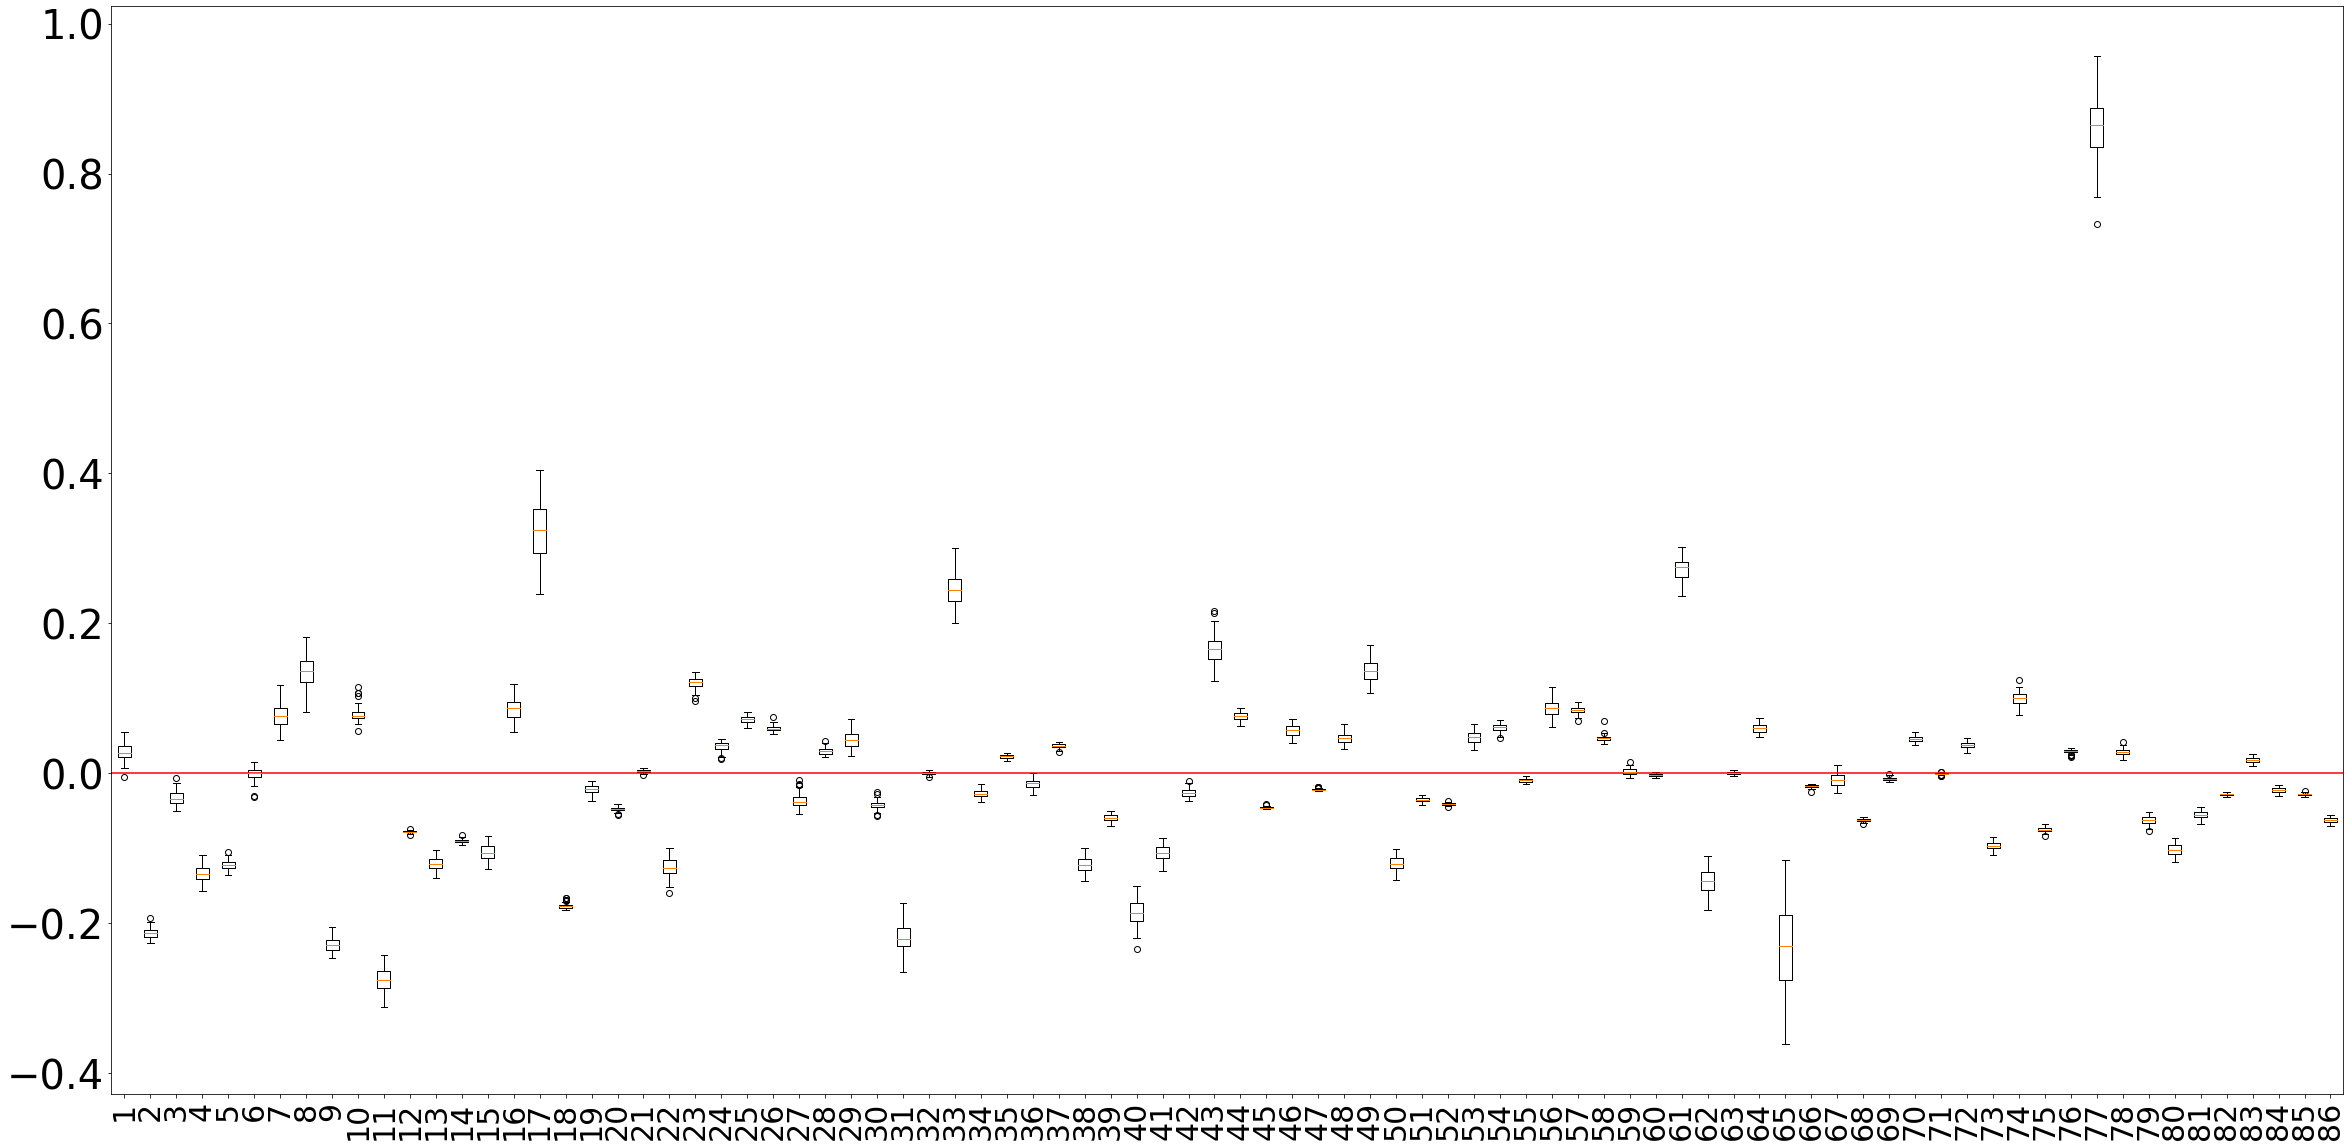
\includegraphics[width=1\linewidth]{figures/distribution_mean_beta_only_top95_fs.png}
\caption{ Distribution of mean (average over 5 folds) beta coefficients for all regions in fs86-ChaCo models. Regions are listed on the x-axis and beta values on the y-axis.}
\label{fs_beta_coeffs}
\end{figure}

\begin{figure}[htp]
\centering
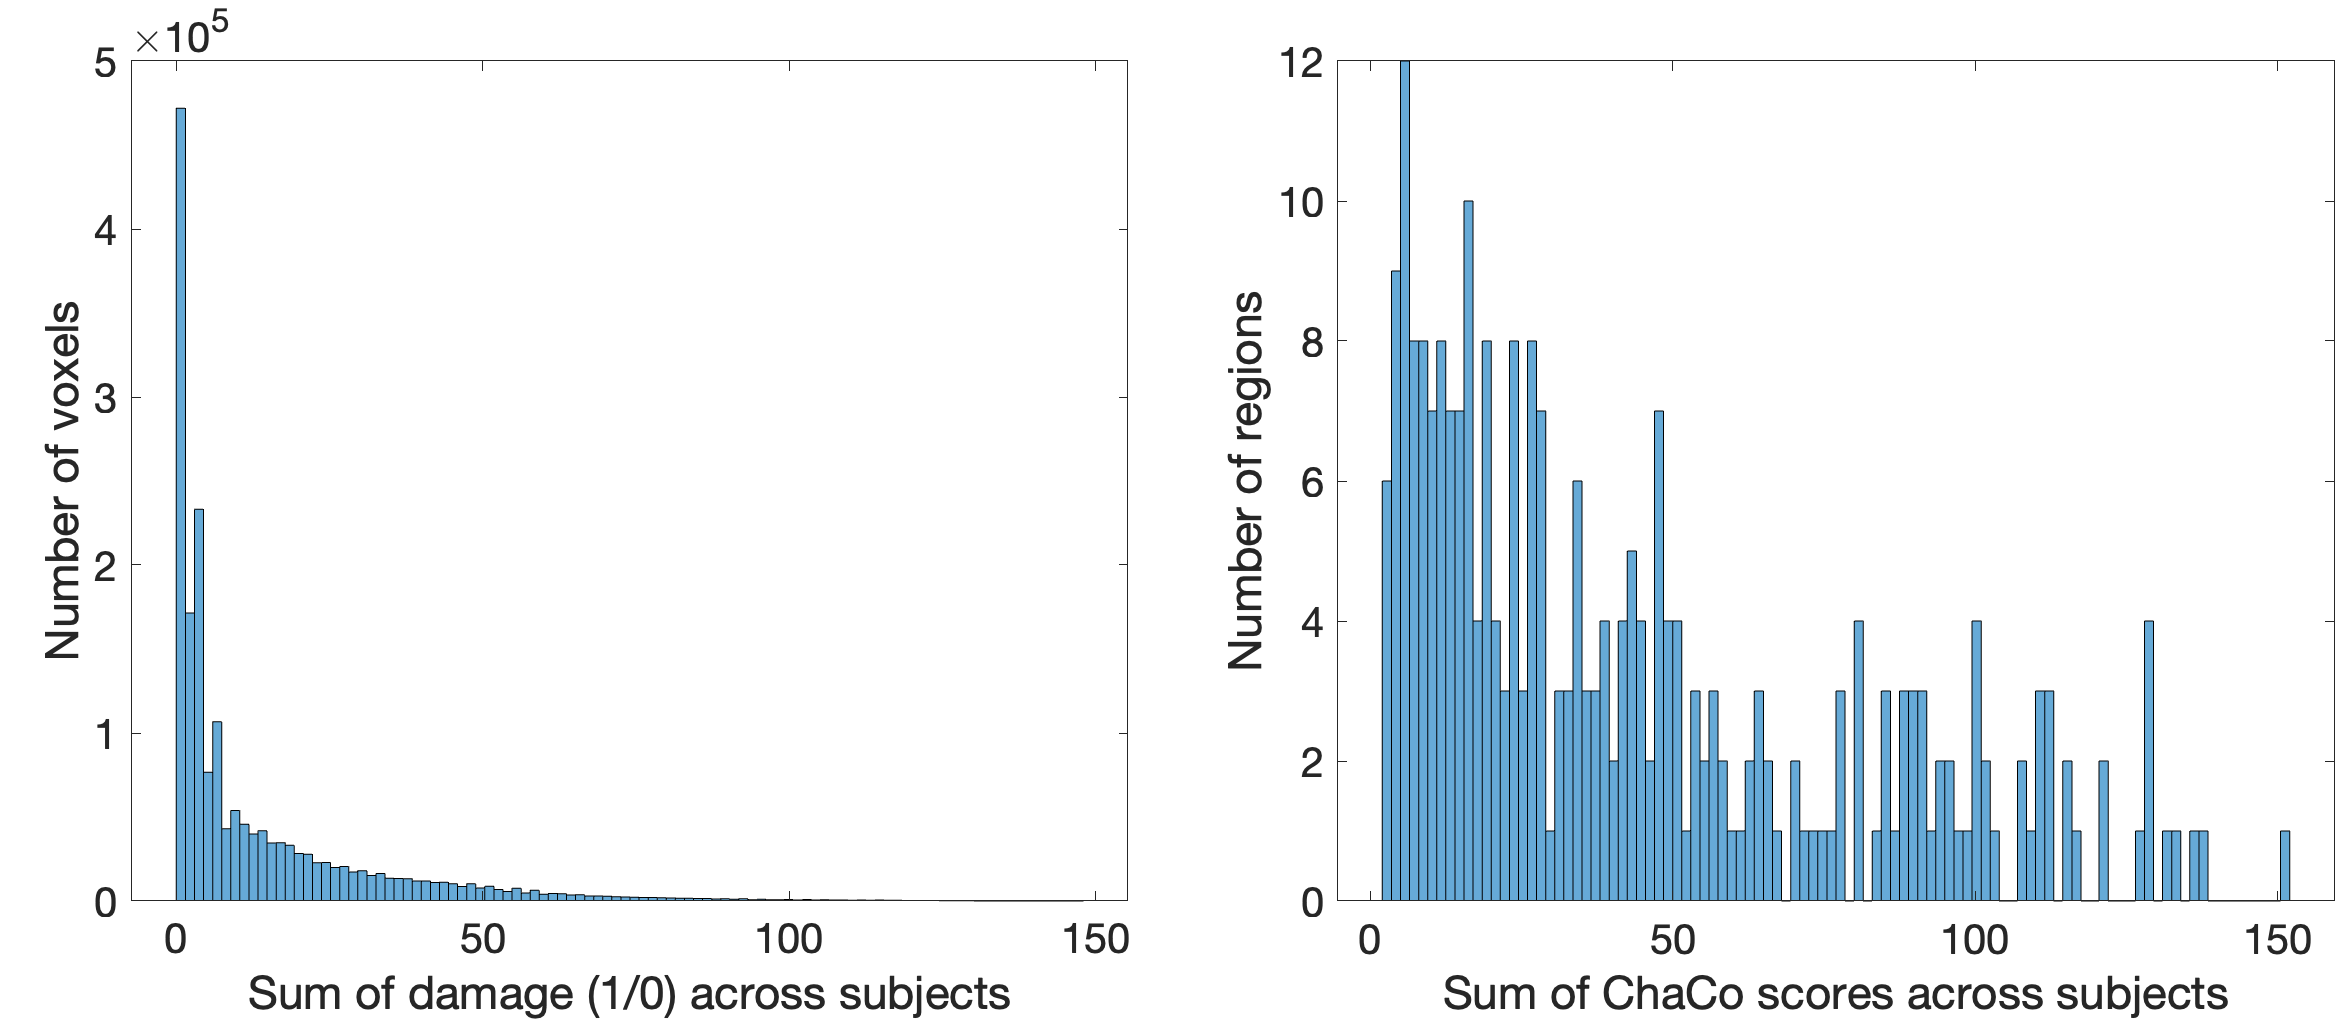
\includegraphics[width=1\linewidth]{figures/histogram_voxels_chaco.png}
\caption{Histogram of voxelwise lesion damage and regional (ChaCo scores) lesion damage. Left:  Distribution of voxelwise lesion damage within a whole-brain mask. Most voxels are damaged in zero subjects. Right: Distribution of ChaCo scores across all subjects. Every region has some disconnection in at least one subject in the population. }
\label{histogram_voxels_chaco}
\end{figure}


\end{document}